\newpage
\section{Casi d'uso}
Vengono elencati i casi d'uso ricavati dall'analisi del capitolato C1.

\subsection{Attori}
Di seguito è riportata la gerarchia degli attori individuati. L'utente generico viene utilizzato nei diagrammi UML per indicare funzionalità fruibili indipendentemente dallo status di autenticazione. Successivamente la gerarchia distingue il cliente (cioè un utente autenticato) dall'utente non autenticato. Il cliente accede solo ai servizi base di API Market, in particolare la ricerca e l'acquisto di API. Lo sviluppatore è un cliente che può registrare nuove API e trarne profitto. L'amministratore API Market è uno sviluppatore che possiede funzionalità di amministrazione della piattaforma.

\label{Attori}

\begin{figure}[ht]
	\centering
	\includegraphics[scale=0.45]{UML/Attori.png}
	\caption{Attori}
\end{figure}


\newpage
\subsection{Caso d'uso UC1: Main pre-autenticazione}
\label{UC1}
\begin{figure}[ht]
	\centering
	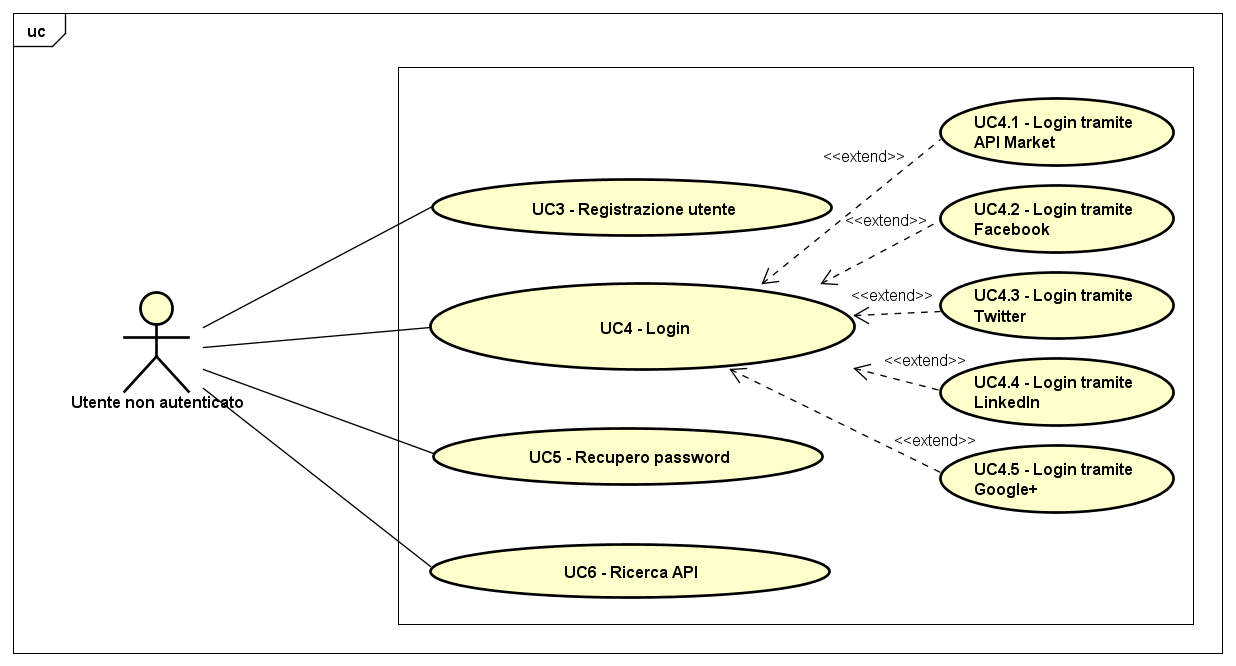
\includegraphics[scale=0.45]{UML/UC1.png}
	\caption{UC1: Main pre-autenticazione}
\end{figure}

\renewcommand*{\arraystretch}{1.6}
\begin{longtable}{ l | p{11cm}}
	\hline
	\rowcolor{Gray}
	\multicolumn{2}{c}{UC1 - Main pre-autenticazione} \\
	\hline
	\textbf{Attori} & Utente non autenticato  \\
	\textbf{Descrizione} & L'attore si trova nella schermata principale dell'applicazione ed accede alle funzionalità a lui disponibili: la registrazione, il login, il recupero password, la ricerca API \\
	\textbf{Pre-Condizioni} & L'attore ha avviato l'applicazione web e non si è ancora autenticato \\
	\textbf{Post-Condizioni} & L'applicazione ha eseguito le richieste dell'attore \\
	\textbf{Scenario Principale} & 
	\begin{enumerate*}[label=(\arabic*.),itemjoin={\newline}]
		\item L'attore può registrarsi all'applicazione (UC3)
		\item L'attore può effettuare il login all'applicazione (UC4)
		\item L'attore può recuperare la propria password (UC5)
		\item L'attore può effettuare una ricerca sulle API presenti nell'applicazione (UC6)
	\end{enumerate*}\\
	\textbf{Scenari Alternativi} & 
	\begin{enumerate*}[label=(\arabic*.),itemjoin={\newline}]
		\item L'attore può effettuare il login tramite API Market (UC4.1)
		\item L'attore può effettuare il login tramite Facebook (UC4.2)
		\item L'attore può effettuare il login tramite Twitter (UC4.3)
		\item L'attore può effettuare il login tramite LinkedIn (UC4.4)
		\item L'attore può effettuare il login tramite Google+ (UC4.5)
	\end{enumerate*}\\
\end{longtable}
\newpage
\subsection{Caso d'uso UC2: Main post-autenticazione }
\label{UC2}
\begin{figure}[ht]
	\centering
	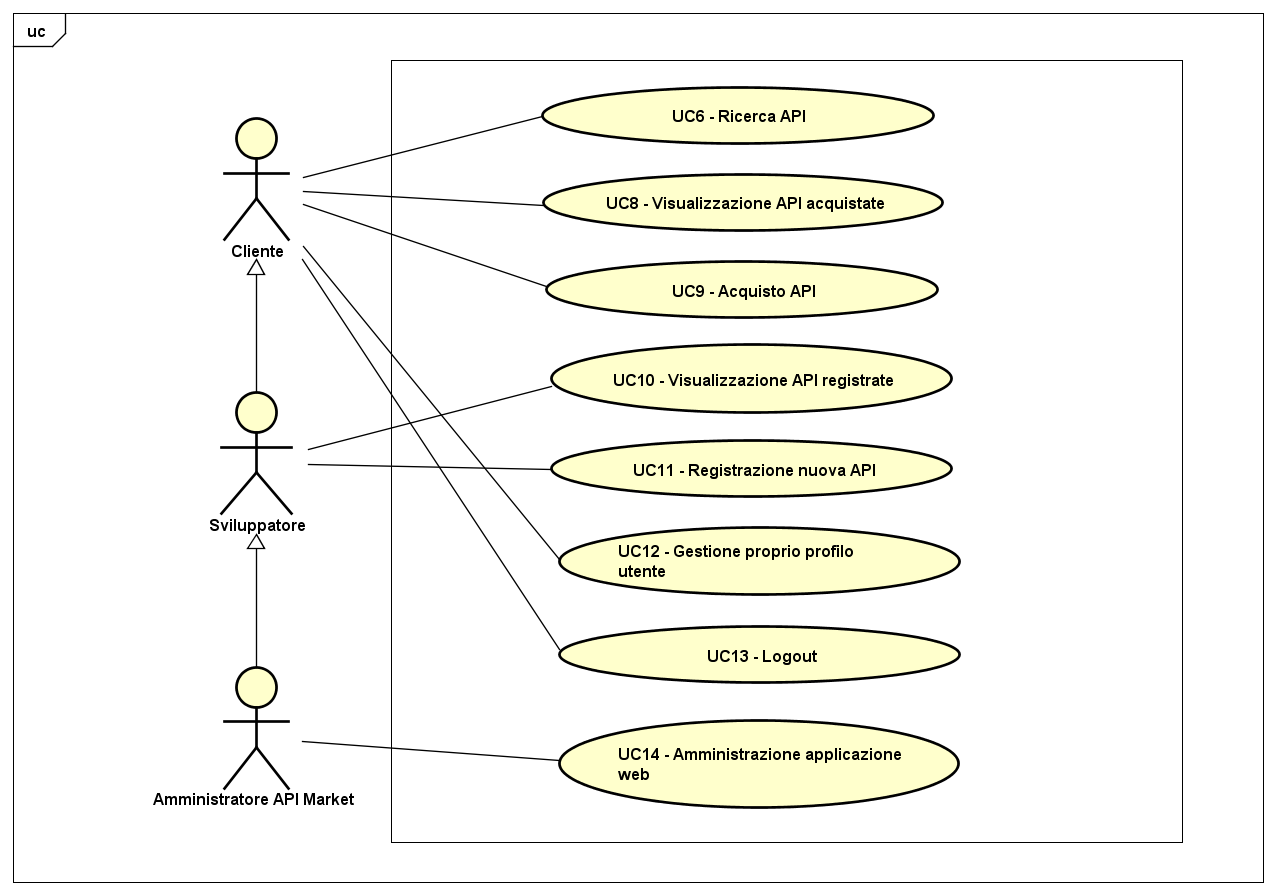
\includegraphics[scale=0.45]{UML/UC2.png}
	\caption{UC2: Main post-autenticazione}
\end{figure}

\begin{longtable}{ l | p{11cm}}
	\hline
	\rowcolor{Gray}
	 \multicolumn{2}{c}{UC2 - Main post-autenticazione} \\
	 \hline
	\textbf{Attori} & Cliente, Sviluppatore, Amministratore API Market \\
	\textbf{Descrizione} & Il cliente, tramite la schermata principale dell'applicazione, può accedere e sfruttare le funzionalità a lui disponibili: la ricerca API, la visualizzazione di API acquistate, l'acquisto API, la gestione del proprio profilo utente, il logout.
	Lo sviluppatore inoltre può visualizzare le API registrate e registrarne di nuove.
	L'amministratore API Market può effettuare una ricerca API ed amministrare l'applicazione web. \\
	\textbf{Pre-Condizioni} & L'attore ha avviato l'applicazione web e si è autenticato. La piattaforma mostra le pagine preposte agli utenti autenticati \\
	\textbf{Post-Condizioni} & L'applicazione ha eseguito le richieste dell'attore \\
	\textbf{Scenario Principale} & 
	\begin{enumerate*}[label=(\arabic*.),itemjoin={\newline}]
		\item L'attore può effettuare una ricerca sulle API presenti nell'applicazione
(UC6)
		\item Il cliente può visualizzare le API da lui acquistate (UC8)
		\item Il cliente può acquistare una API (UC9)
		\item Lo sviluppatore può visualizzare le API da lui registrate (UC10)
		\item Lo sviluppatore può registrare una nuova API (UC11)
		\item Il cliente può gestire il proprio profilo utente (UC12)
		\item L'attore può effettuare il logout (UC13)
		\item L'amministratore API Market può accedere all'amministrazione dell'applicazione web (UC14)
	\end{enumerate*}\\
\end{longtable}
\newpage
\subsection{Caso d'uso UC3: Registrazione utente }
\label{UC3}
\begin{figure}[ht]
	\centering
	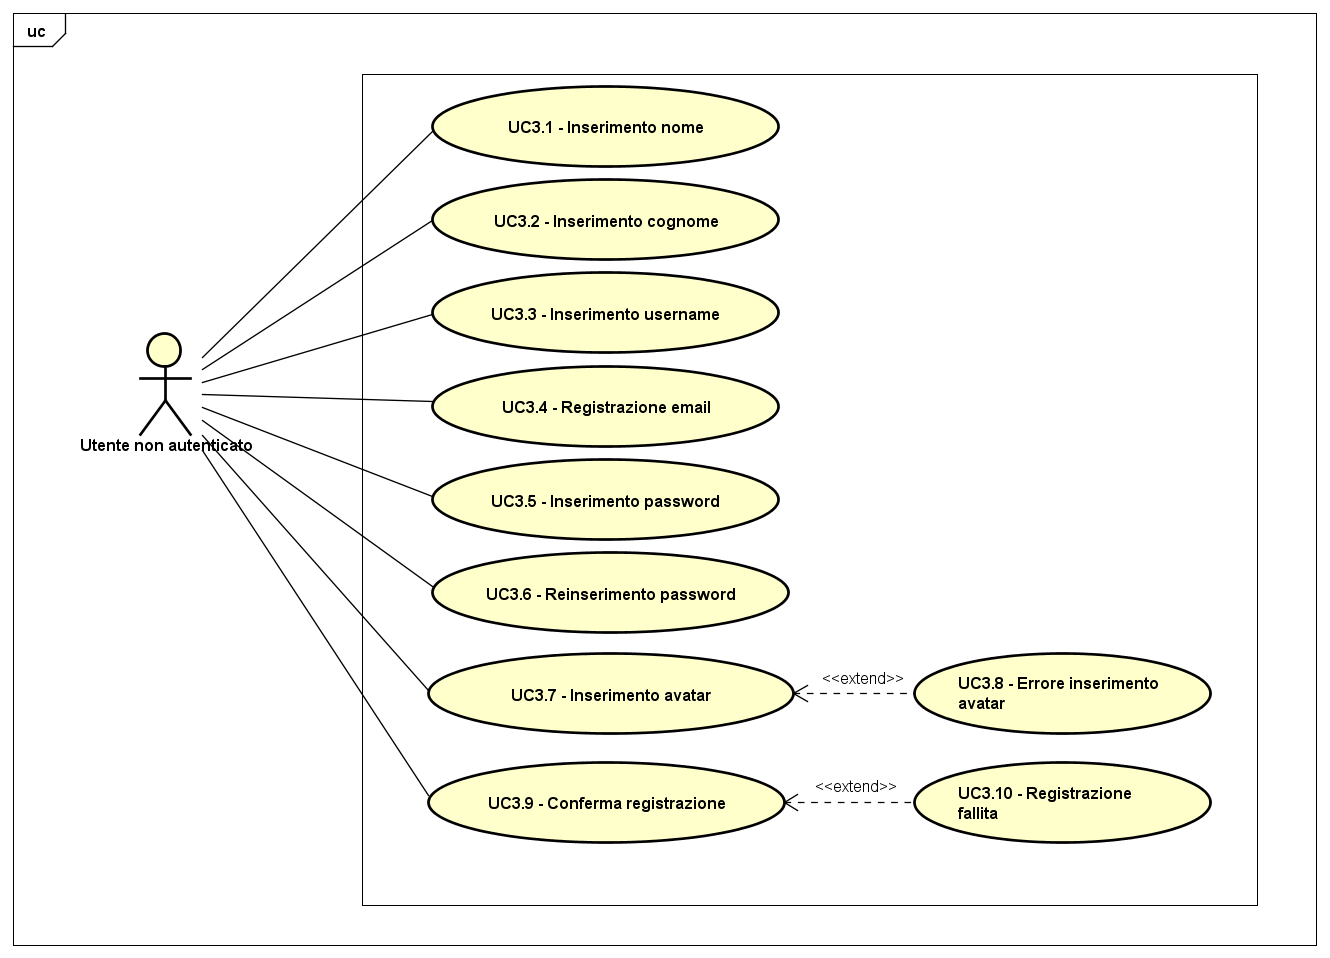
\includegraphics[scale=0.45]{UML/UC3.png}
	\caption{UC3: Registrazione utente}
\end{figure}

\begin{longtable}{ l | p{11cm}}
	\hline
	\rowcolor{Gray}
	 \multicolumn{2}{c}{UC3 - Registrazione utente} \\
	 \hline
	\textbf{Attori} & Utente non autenticato \\
	\textbf{Descrizione} & L'attore inserisce le sue informazioni personali per potersi registrare all'applicazione web, così da poter successivamente effettuare il login ed evolversi in un utente autenticato. \\
	\textbf{Pre-Condizioni} & L'attore ha scelto di registrarsi e l'applicazione web mostra la schermata di registrazione \\
	\textbf{Post-Condizioni} & L'attore si è registrato all'applicazione web \\
	\textbf{Scenario Principale} & 
	\begin{enumerate*}[label=(\arabic*.),itemjoin={\newline}]
		\item L'attore può inserire il proprio nome (UC3.1)
		\item L'attore può inserire il proprio cognome (UC3.2)
		\item L'attore può inserire lo username desiderato (UC3.3)
		\item L'attore può inserire la propria email (UC3.4) 
		\item L'attore può inserire la password desiderata (UC3.5)
		\item L'attore può reinserire la password desiderata per conferma (UC3.6)
		\item L'attore può inserire il proprio avatar (UC3.7)
		\item L'attore può confermare la registrazione (UC3.9)
	\end{enumerate*}\\
	\textbf{Scenari Alternativi} & 
	\begin{enumerate*}[label=(\arabic*.),itemjoin={\newline}]
		\item L'attore può visualizzare un messaggio di errore riguardo al caricamento del file dell'avatar del nuovo utente, ed il caricamento del file non avviene (UC3.8)
		\item L'attore può visualizzare un messaggio d'errore che segnala i campi dati non validi (UC3.10)
	\end{enumerate*}\\
\end{longtable}

\subsubsection{Caso d'uso UC3.1: Inserimento nome}
\label{UC3_1}

\begin{longtable}{ l | p{11cm}}
	\hline
	\rowcolor{Gray}
	 \multicolumn{2}{c}{UC3.1 - Inserimento nome} \\
	 \hline
	\textbf{Attori} & Utente non autenticato \\
	\textbf{Descrizione} & L'attore inserisce il suo nome \\
	\textbf{Pre-Condizioni} & L'applicazione mostra il campo dati per l'inserimento del nome \\
	\textbf{Post-Condizioni} & L'attore ha inserito il proprio nome \\
	\textbf{Scenario Principale} & 
	\begin{enumerate*}[label=(\arabic*.),itemjoin={\newline}]
		\item L'attore può inserire il proprio nome
	\end{enumerate*}\\
\end{longtable}

\subsubsection{Caso d'uso UC3.2: Inserimento cognome}
\label{UC3_2}

\begin{longtable}{ l | p{11cm}}
	\hline
	\rowcolor{Gray}
	 \multicolumn{2}{c}{UC3.2 - Inserimento cognome} \\
	 \hline
	\textbf{Attori} & Utente non autenticato \\
	\textbf{Descrizione} & L'attore inserisce il suo cognome \\
	\textbf{Pre-Condizioni} & L'applicazione mostra il campo dati per l'inserimento del cognome \\
	\textbf{Post-Condizioni} & L'attore ha inserito il proprio cognome \\
	\textbf{Scenario Principale} & 
	\begin{enumerate*}[label=(\arabic*.),itemjoin={\newline}]
		\item L'attore può inserire il proprio cognome
	\end{enumerate*}\\
\end{longtable}

\subsubsection{Caso d'uso UC3.3: Inserimento username}
\label{UC3_3}

\begin{longtable}{ l | p{11cm}}
	\hline
	\rowcolor{Gray}
	 \multicolumn{2}{c}{UC3.3: Inserimento username} \\
	 \hline
	\textbf{Attori} & Utente non autenticato \\
	\textbf{Descrizione} & L'attore inserisce lo username desiderato \\
	\textbf{Pre-Condizioni} & L'applicazione mostra il campo dati per l'inserimento dello username \\
	\textbf{Post-Condizioni} & L'attore ha inserito lo username desiderato \\
	\textbf{Scenario Principale} & 
	\begin{enumerate*}[label=(\arabic*.),itemjoin={\newline}]
		\item L'attore può inserire lo username desiderato
	\end{enumerate*}\\
\end{longtable}

\subsubsection{Caso d'uso UC3.4: Registrazione email}
\label{UC3_4}

\begin{longtable}{ l | p{11cm}}
	\hline
	\rowcolor{Gray}
	 \multicolumn{2}{c}{UC3.4 - Registrazione email} \\
	 \hline
	\textbf{Attori} & Utente non autenticato \\
	\textbf{Descrizione} & L'attore registra la propria email \\
	\textbf{Pre-Condizioni} & L'applicazione mostra il campo dati per la registrazione dell'email \\
	\textbf{Post-Condizioni} & L'attore ha registrato la propria email \\
	\textbf{Scenario Principale} & 
	\begin{enumerate*}[label=(\arabic*.),itemjoin={\newline}]
		\item L'attore può registrare la propria email
	\end{enumerate*}
\end{longtable}

\subsubsection{Caso d'uso UC3.5: Inserimento password}
\label{UC3_5}

\begin{longtable}{ l | p{11cm}}
	\hline
	\rowcolor{Gray}
	 \multicolumn{2}{c}{UC3.5 - Inserimento password} \\
	 \hline
	\textbf{Attori} & Utente non autenticato \\
	\textbf{Descrizione} & L'attore inserisce la password desiderata  \\
	\textbf{Pre-Condizioni} & L'applicazione mostra il campo dati per l'inserimento della password \\
	\textbf{Post-Condizioni} & L'attore ha inserito la password desiderata \\
	\textbf{Scenario Principale} & 
	\begin{enumerate*}[label=(\arabic*.),itemjoin={\newline}]
		\item L'attore può inserire la password desiderata
	\end{enumerate*}\\
\end{longtable}

\subsubsection{Caso d'uso UC3.6: Reinserimento password}
\label{UC3_6}

\begin{longtable}{ l | p{11cm}}
	\hline
	\rowcolor{Gray}
	 \multicolumn{2}{c}{UC3.6 - Reinserimento password} \\
	 \hline
	\textbf{Attori} & Utente non autenticato \\
	\textbf{Descrizione} & L'attore reinserisce la password desiderata  \\
	\textbf{Pre-Condizioni} & L'applicazione mostra il campo dati per il reinserimento della password \\
	\textbf{Post-Condizioni} & L'attore ha reinserito la password desiderata \\
	\textbf{Scenario Principale} & 
	\begin{enumerate*}[label=(\arabic*.),itemjoin={\newline}]
		\item L'attore può reinserire la password desiderata
	\end{enumerate*}\\
\end{longtable}

\subsubsection{Caso d'uso UC3.7: Inserimento avatar}
\label{UC3_7}

\begin{minipage}{\linewidth}
	\begin{tabular}{ l | p{11cm}}
		\hline
		\rowcolor{Gray}
		\multicolumn{2}{c}{UC3.7 - Inserimento avatar} \\
		\hline
		\textbf{Attori} & Utente autenticato, Amministratore API Market \\
		\textbf{Descrizione} & L'attore carica su API Market un file contenente l'avatar per il nuovo utente \\
		\textbf{Pre-Condizioni} & L'attore si trova nella schermata relativa alla registrazione di un nuovo utente \\
		\textbf{Post-Condizioni} & L'attore ha caricato su API Market un file contenente l'avatar per il nuovo utente \\
		\textbf{Scenario Principale} & 
		\begin{enumerate*}[label=(\arabic*.),itemjoin={\newline}]
			\item L'attore può caricare su API Market un file contenente l'avatar per il nuovo utente
		\end{enumerate*}\\
		\textbf{Scenari Alternativi} & 
		\begin{enumerate*}[label=(\arabic*.),itemjoin={\newline}]
		\item L'attore può visualizzare un messaggio di errore (E.g: formato errato) ed il caricamento del file non avviene (UC3.8)
		\end{enumerate*}\\
	\end{tabular}
\end{minipage}

\subsubsection{Caso d'uso UC3.8: Errore inserimento avatar}
\label{UC3_8}

\begin{minipage}{\linewidth}
	\begin{tabular}{ l | p{11cm}}
		\hline
		\rowcolor{Gray}
		\multicolumn{2}{c}{UC3.8 - Errore inserimento avatar} \\
		\hline
		\textbf{Attori} & Utente autenticato, Amministratore API Market \\
		\textbf{Descrizione} & L'attore visualizza un messaggio di errore e l'inserimento dell'avatar per il nuovo utente non avviene \\
		\textbf{Pre-Condizioni} & L'attore ha cercato di caricare su API Market un file contenente l'avatar per il nuovo utente ma si è verificato un errore \\
		\textbf{Post-Condizioni} & L'attore ha visualizzato un messaggio di errore \\
		\textbf{Scenario Principale} & 
		\begin{enumerate*}[label=(\arabic*.),itemjoin={\newline}]
			\item L'attore può visualizzare un messaggio di errore (E.g: formato non valido)
		\end{enumerate*}\\
	\end{tabular}
\end{minipage}

\subsubsection{Caso d'uso UC3.9: Conferma registrazione}
\label{UC3_9}

\begin{longtable}{ l | p{11cm}}
	\hline
	\rowcolor{Gray}
	 \multicolumn{2}{c}{UC3.9 - Conferma registrazione} \\
	 \hline
	\textbf{Attori} & Utente non autenticato \\
	\textbf{Descrizione} & L'attore conferma i dati inseriti per la registrazione \\
	\textbf{Pre-Condizioni} & L'applicazione mostra il pulsante per la conferma della registrazione (con le informazioni inserite nei campi dati) \\
	\textbf{Post-Condizioni} & L'attore ha confermato la registrazione, visualizzando il messaggio di successo, ed è stato reindirizzato alla pagina principale come utente non autenticato (UC1) \\
	\textbf{Scenario Principale} & 
	\begin{enumerate*}[label=(\arabic*.),itemjoin={\newline}]
		\item L'attore può confermare la registrazione, visualizzando il messaggio di successo, e venendo reindirizzato alla pagina principale come utente non autenticato (UC1)
	\end{enumerate*}\\
\end{longtable}

\subsubsection{Caso d'uso UC3.10: Registrazione fallita}
\label{UC3_10}

\begin{minipage}{\linewidth}
	\begin{longtable}{ l | p{11cm}}
		\hline
		\rowcolor{Gray}
	 	\multicolumn{2}{c}{UC3.10 - Registrazione fallita} \\
	 	\hline
		\textbf{Attori} & Utente non autenticato \\
		\textbf{Descrizione} & L'attore fallisce la registrazione  \\
		\textbf{Pre-Condizioni} & L'attore ha confermato i dati inseriti \\
		\textbf{Post-Condizioni} & L'attore ha visualizzato un messaggio d'errore che segnala i campi dati non validi \\
		\textbf{Scenario Principale} & 
		\begin{enumerate*}[label=(\arabic*.),itemjoin={\newline}]
			\item L'attore può visualizzare un messaggio d'errore che segnala i campi dati non validi (E.g: Campi dati vuoti, caratteri speciali, username o email già presenti) 
		\end{enumerate*}\\
	\end{longtable}
\end{minipage}
\newpage
\subsection{Caso d'uso UC4: Login}
\label{UC4}

\begin{longtable}{ l | p{11cm}}
	\hline
	\rowcolor{Gray}
	 \multicolumn{2}{c}{UC4 - Login}\\
	 \hline
	\textbf{Attori} & Utente non autenticato \\
	\textbf{Descrizione} & L'attore inserisce le sue informazioni personali per poter accedere all'applicazione web ed evolversi in un utente autenticato \\
	\textbf{Pre-Condizioni} & L'attore si trova nella schermata iniziale dell'applicazione web \\
	\textbf{Post-Condizioni} & L'attore ha effettuato l'accesso all'applicazione web \\
	\textbf{Scenario Principale} & 
	\begin{enumerate*}[label=(\arabic*.),itemjoin={\newline}]
		\item L'attore può effettuare il login all'applicazione web
	\end{enumerate*}\\
\end{longtable}
\newpage
\subsubsection{Caso d'uso UC4.1: Login tramite API Market}
\label{UC4_1}
\begin{figure}[!htbp]
	\centering
	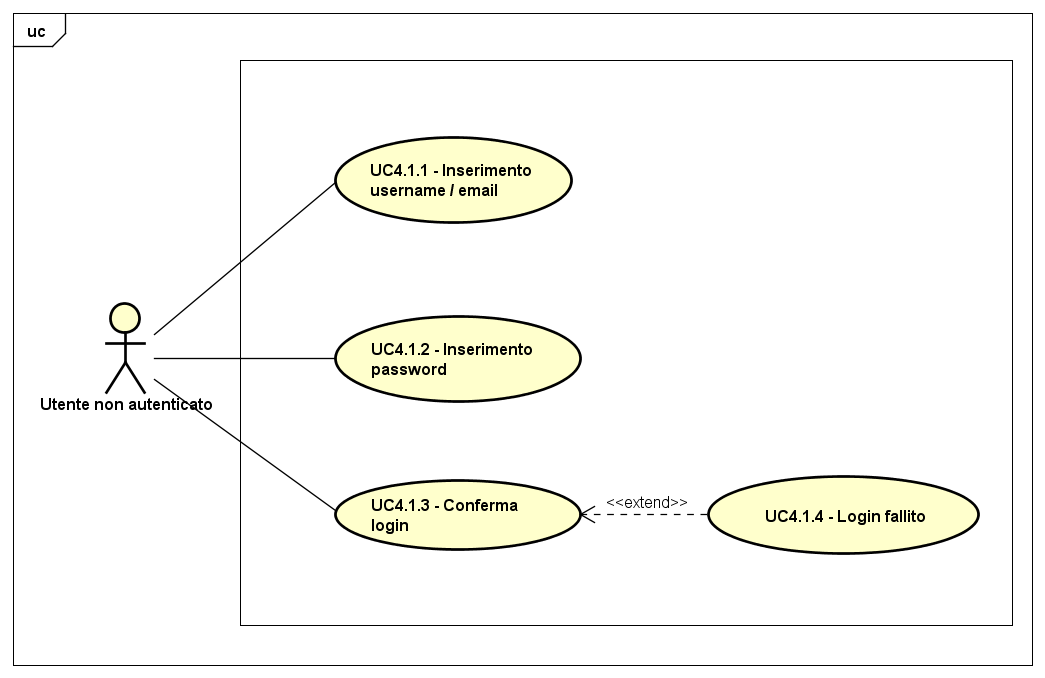
\includegraphics[scale=0.45]{UML/UC4_1.png}
	\caption{UC4.1: Login tramite API Market}
\end{figure}

\begin{tabular}{ l | p{11cm}}
	\hline
	\rowcolor{Gray}
	 \multicolumn{2}{c}{UC4.1 - Login tramite API Market} \\
	 \hline
	\textbf{Attori} & Utente non autenticato \\
	\textbf{Descrizione} & L'attore effettua il login all'applicazione web, così da evolversi in un utente autenticato\\
	\textbf{Pre-Condizioni} & L'attore ha scelto di eseguire il login all'applicazione web (e non è autenticato) \\
	\textbf{Post-Condizioni} & L'attore ha effettuato il login all'applicazione web, evolvendosi in un utente autenticato \\
	\textbf{Scenario Principale} & 
	\begin{enumerate*}[label=(\arabic*.),itemjoin={\newline}]
		\item L'attore può inserire il proprio username o la propria email (UC4.1.1)
		\item L'attore può inserire la propria password (UC4.1.2)
		\item L'attore può confermare il login e autenticarsi (UC4.1.3)
	\end{enumerate*}\\
	\textbf{Scenari Alternativi} & 
	\begin{enumerate*}[label=(\arabic*.),itemjoin={\newline}]
		\item L'attore può fallire il login e visualizzare un relativo messaggio d'errore (UC4.1.4)
	\end{enumerate*}\\
\end{tabular}


\paragraph{Caso d'uso UC4.1.1: Inserimento username / email}
\label{UC4_1_1}

\begin{minipage}{\linewidth}
\begin{longtable}{ l | p{11cm}}
	\hline
	\rowcolor{Gray}
	\multicolumn{2}{c}{UC4.1.1: Inserimento username / email} \\
	\hline
	\textbf{Attori} & Utente non autenticato \\
	\textbf{Descrizione} & L'attore inserisce il proprio username o la propria email  \\
	\textbf{Pre-Condizioni} & L'applicazione mostra il campo dati per l'inserimento dello username o dell'email \\
	\textbf{Post-Condizioni} & L'attore ha inserito il proprio username o la propria email \\
	\textbf{Scenario Principale} & 
	\begin{enumerate*}[label=(\arabic*.),itemjoin={\newline}]
		\item L'attore può inserire il proprio username o la propria email
	\end{enumerate*}\\
\end{longtable}
\end{minipage}


\paragraph{Caso d'uso UC4.1.2: Inserimento password}
\label{UC4_1_2}

\begin{minipage}{\linewidth}
\begin{longtable}{ l | p{11cm}}
	\hline
	\rowcolor{Gray}
	\multicolumn{2}{c}{UC4.1.2: Inserimento password} \\
	\hline
	\textbf{Attori} & Utente non autenticato \\
	\textbf{Descrizione} & L'attore inserisce la propria password  \\
	\textbf{Pre-Condizioni} & L'applicazione mostra il campo dati per l'inserimento della password \\
	\textbf{Post-Condizioni} & L'attore ha inserito la propria password \\
	\textbf{Scenario Principale} & 
	\begin{enumerate*}[label=(\arabic*.),itemjoin={\newline}]
		\item L'utente non autenticato può inserire la propria password
	\end{enumerate*}\\
\end{longtable}
\end{minipage}


\paragraph{Caso d'uso UC4.1.3: Conferma Login}
\label{UC4_1_3}

\begin{minipage}{\linewidth}
\begin{longtable}{ l | p{11cm}}
	\hline
	\rowcolor{Gray}
	\multicolumn{2}{c}{UC4.1.3: Conferma Login} \\
	\hline
	\textbf{Attori} & Utente non autenticato \\
	\textbf{Descrizione} & L'attore conferma i dati inseriti per il login \\
	\textbf{Pre-Condizioni} & L'applicazione mostra il pulsante per la conferma del login (con le informazioni inserite nei campi dati) \\
	\textbf{Post-Condizioni} & L'attore ha confermato il login, visualizzando il messaggio di successo, ed è stato reindirizzato alla pagina principale evolvendosi in un utente autenticato (UC2) \\
	\textbf{Scenario Principale} & 
	\begin{enumerate*}[label=(\arabic*.),itemjoin={\newline}]
	\item L'attore può confermare il login, visualizzando il messaggio di successo, e venendo reindirizzato alla pagina principale evolvendosi in un utente autenticato (UC2)
\end{enumerate*}\\
\end{longtable}
\end{minipage}

\paragraph{Caso d'uso UC4.1.4: Login fallito}
\label{UC4_1_4}

\begin{minipage}{\linewidth}
\begin{longtable}{ l | p{11cm}}
	\hline
	\rowcolor{Gray}
	\multicolumn{2}{c}{UC4.1.4: Login fallito} \\
	\hline
	\textbf{Attori} & Utente non autenticato \\
	\textbf{Descrizione} & L'attore ha fallito il login  \\
	\textbf{Pre-Condizioni} & L'attore ha confermato i dati inseriti \\
	\textbf{Post-Condizioni} & L'attore visualizza un messaggio d'errore \\
	\textbf{Scenario Principale} & 
	\begin{enumerate*}[label=(\arabic*.),itemjoin={\newline}]
		\item L'attore visualizza un messaggio d'errore relativo al fallimento della procedura
	\end{enumerate*}\\
\end{longtable}
\end{minipage}
\newpage
\subsubsection{Caso d'uso UC4.2: Login tramite Facebook }
\label{UC4_2}
\begin{figure}[!htbp]
	\centering
	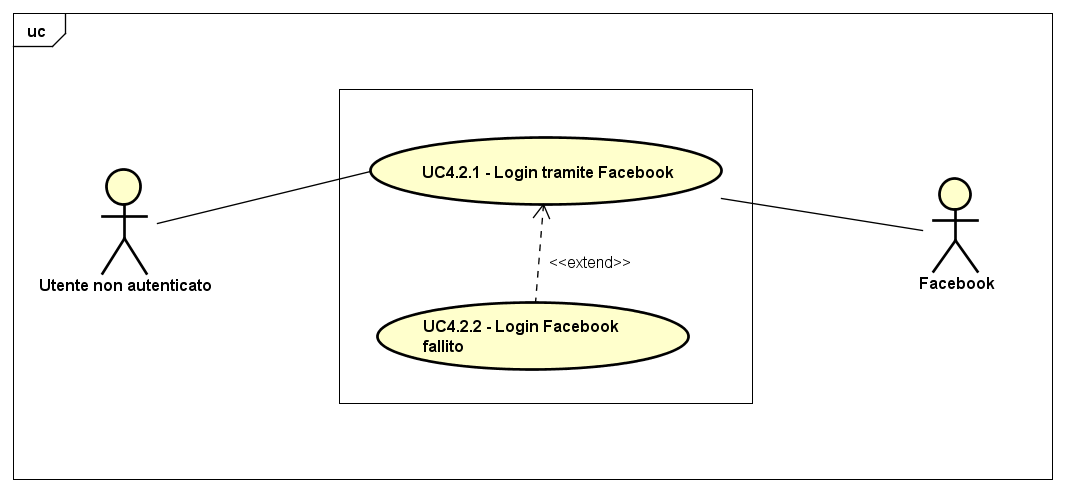
\includegraphics[scale=0.45]{UML/UC4_2.png}
	\caption{UC4.2: Login tramite Facebook}
\end{figure}

\begin{tabular}{ l | p{11cm}}
	\hline
	\rowcolor{Gray}
	 \multicolumn{2}{c}{UC4.2 - Login tramite Facebook} \\
	 \hline
	\textbf{Attori} & Utente non autenticato, Facebook \\
	\textbf{Descrizione} & L'attore effettua il login all'applicazione web tramite Facebook, così da evolversi in un utente autenticato \\
	\textbf{Pre-Condizioni} & L'attore ha scelto di eseguire il login all'applicazione web tramite Facebook (e non è autenticato). L'applicazione mostra la schermata per gli utenti non autenticati. \\
	\textbf{Post-Condizioni} & L'attore ha effettuato il login all'applicazione web tramite Facebook, evolvendosi in un utente autenticato \\
	\textbf{Scenario Principale} & 
	\begin{enumerate*}[label=(\arabic*.),itemjoin={\newline}]
		\item L'attore può effettuare con successo il login tramite Facebook (UC4.2.1), visualizzando un messaggio di successo, e venendo reindirizzato alla pagina principale evolvendosi in un utente autenticato (UC2)
	\end{enumerate*}\\
	\textbf{Scenari Alternativi} & 
	\begin{enumerate*}[label=(\arabic*.),itemjoin={\newline}]
	\item L'attore ha fallito il login tramite Facebook (E.g: Mancanza di privilegi/autorizzazioni, problemi legati a Facebook...) e visualizza un messaggio d'errore (UC4.2.2)
	\end{enumerate*}\\
\end{tabular}
\newpage
\subsubsection{Caso d'uso UC4.3: Login tramite Twitter }
\label{UC4_3}
\begin{figure}[!htbp]
	\centering
	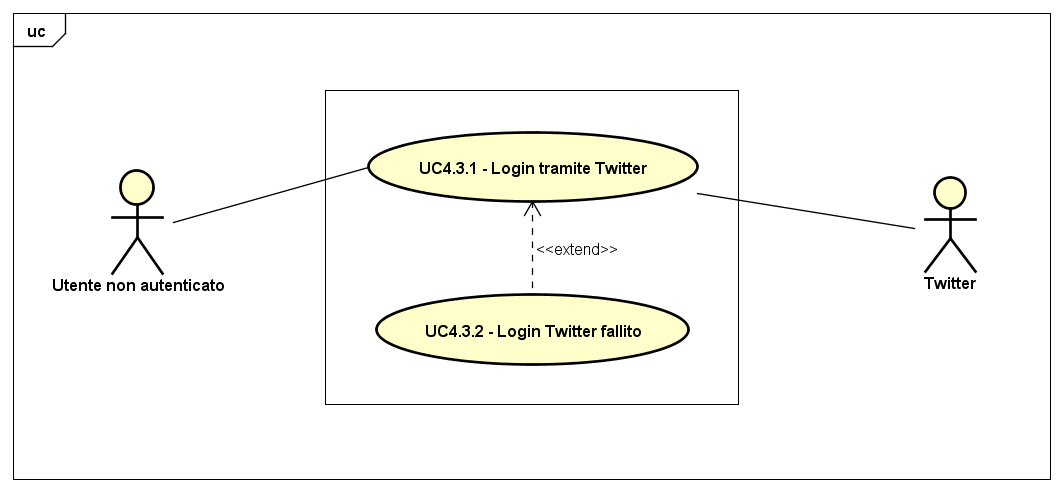
\includegraphics[scale=0.45]{UML/UC4_3.png}
	\caption{UC4.3: Login tramite Twitter}
\end{figure}

\begin{tabular}{ l | p{11cm}}
	\hline
	\rowcolor{Gray}
	\multicolumn{2}{c}{UC4.3 - Login tramite Twitter} \\
	\hline
	\textbf{Attori} & Utente non autenticato, Twitter \\
	\textbf{Descrizione} & L'attore effettua il login all'applicazione web tramite Twitter, così da evolversi in un utente autenticato \\
	\textbf{Pre-Condizioni} & L'attore ha scelto di eseguire il login all'applicazione web tramite Twitter (e non è autenticato) \\
	\textbf{Post-Condizioni} & L'attore ha effettuato il login all'applicazione web tramite Twitter, evolvendosi in un utente autenticato \\
	\textbf{Scenario Principale} & 
	\begin{enumerate*}[label=(\arabic*.),itemjoin={\newline}]
		\item L'attore può effettuare con successo il login tramite Twitter (UC4.3.1), visualizzando un messaggio di successo, e venendo reindirizzato alla pagina principale evolvendosi in un utente autenticato (UC2)
	\end{enumerate*}\\
	\textbf{Scenari Alternativi} & 
	\begin{enumerate*}[label=(\arabic*.),itemjoin={\newline}]
	\item L'attore ha fallito il login tramite Twitter (E.g: Mancanza di privilegi/autorizzazioni, problemi legati a Twitter...) e visualizza un messaggio d'errore (UC4.3.2)
	\end{enumerate*}\\
\end{tabular}
\newpage
\subsubsection{Caso d'uso UC4.4: Login tramite LinkedIn }
\label{UC4_4}
\begin{figure}[!htbp]
	\centering
	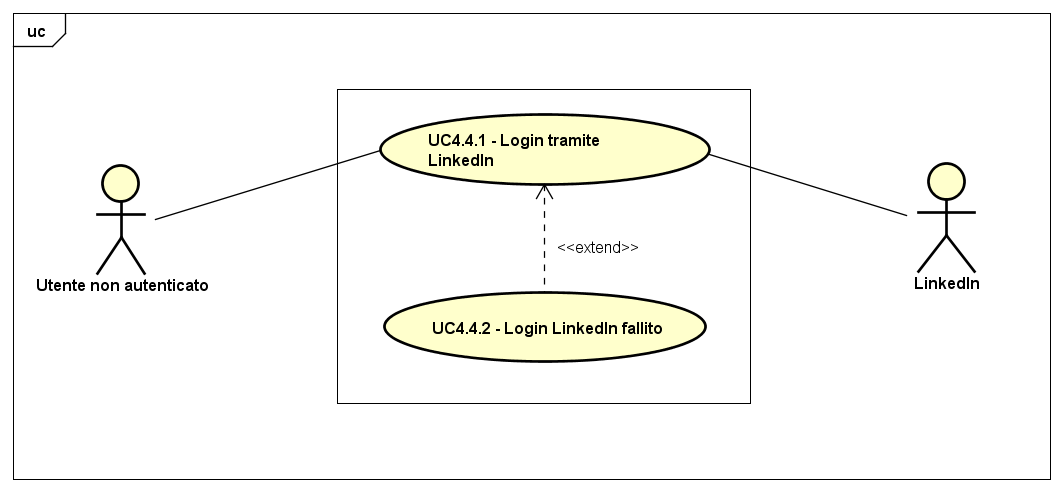
\includegraphics[scale=0.45]{UML/UC4_4.png}
	\caption{UC4.2: Login tramite LinkedIn}
\end{figure}

\begin{tabular}{ l | p{11cm}}
	\hline
	\rowcolor{Gray}
	\multicolumn{2}{c}{UC4.4 - Login tramite LinkedIn} \\
	\hline
	\textbf{Attori} & Utente non autenticato, LinkedIn \\
	\textbf{Descrizione} & L'attore effettua il login all'applicazione web tramite LinkedIn, così da evolversi in un utente autenticato \\
	\textbf{Pre-Condizioni} & L'attore ha scelto di eseguire il login all'applicazione web tramite LinkedIn (e non è autenticato). L'applicazione mostra la schermata per gli utenti non autenticati. \\
	\textbf{Post-Condizioni} & L'attore ha effettuato il login all'applicazione web tramite LinkedIn, evolvendosi in un utente autenticato \\
	\textbf{Scenario Principale} & 
	\begin{enumerate*}[label=(\arabic*.),itemjoin={\newline}]
		\item L'attore può effettuare con successo il login tramite LinkedIn (UC4.4.1), visualizzando un messaggio di successo, e venendo reindirizzato alla pagina principale evolvendosi in un utente autenticato (UC2)
	\end{enumerate*}\\
	\textbf{Scenari Alternativi} & 
	\begin{enumerate*}[label=(\arabic*.),itemjoin={\newline}]
	\item L'attore ha fallito il login tramite LinkedIn (E.g: Mancanza di privilegi/autorizzazioni, utente non correttamente loggato a LinkedIn...) e visualizza un messaggio d'errore (UC4.4.2)
	\end{enumerate*}\\
\end{tabular}
\newpage
\subsubsection{Caso d'uso UC4.5: Login tramite Google+ }
\label{UC4_5}
\begin{figure}[!htbp]
	\centering
	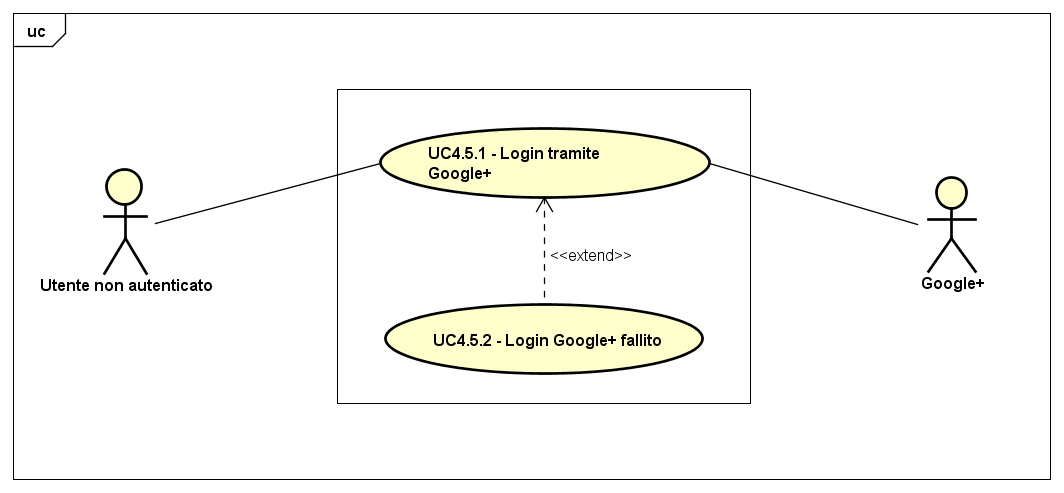
\includegraphics[scale=0.45]{UML/UC4_5.png}
	\caption{UC4.5: Login tramite Google+}
\end{figure}

\begin{tabular}{ l | p{11cm}}
	\hline
	\rowcolor{Gray}
	\multicolumn{2}{c}{UC4.5 - Login tramite Google+} \\
	\hline
	\textbf{Attori} & Utente non autenticato, Google+ \\
	\textbf{Descrizione} & L'attore effettua il login all'applicazione web tramite Google+, così da evolversi in un utente autenticato \\
	\textbf{Pre-Condizioni} & L'attore ha scelto di eseguire il login all'applicazione web tramite Google+ (e non è autenticato) \\
	\textbf{Post-Condizioni} & L'attore ha effettuato il login all'applicazione web tramite Google+, evolvendosi in un utente autenticato \\
	\textbf{Scenario Principale} & 
	\begin{enumerate*}[label=(\arabic*.),itemjoin={\newline}]
		\item L'attore può effettuare con successo il login tramite Google+ (UC4.5.1), visualizzando un messaggio di successo, e venendo reindirizzato alla pagina principale evolvendosi in un utente autenticato (UC2)
	\end{enumerate*}\\
	\textbf{Scenari Alternativi} & 
	\begin{enumerate*}[label=(\arabic*.),itemjoin={\newline}]
	\item L'attore ha fallito il login tramite Google+ (E.g: Mancanza di privilegi/autorizzazioni, utente non correttamente loggato a Google+...) e visualizza un messaggio d'errore (4.5.2)
	\end{enumerate*}\\
\end{tabular}
\newpage
\subsection{Caso d'uso UC5: Recupero password}
\label{UC5}
\begin{figure}[ht]
	\centering
	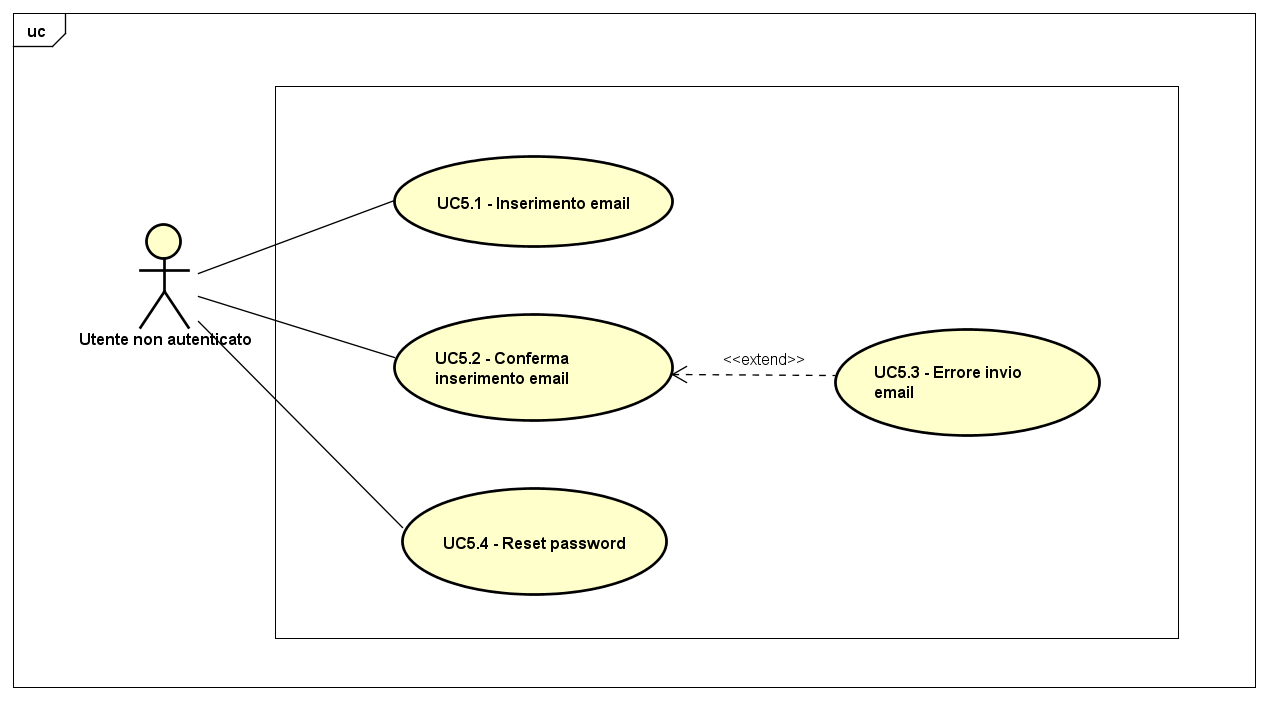
\includegraphics[scale=0.45]{UML/UC5.png}
	\caption{UC5: Recupero password}
\end{figure}

\begin{longtable}{ l | p{11cm}}
	\hline
	\rowcolor{Gray}
	 \multicolumn{2}{c}{UC5 - Recupero password} \\
	 \hline
	\textbf{Attori} & Utente non autenticato \\
	\textbf{Descrizione} & L'attore recupera la password del proprio account API Market tramite l'invio di una email \\
	\textbf{Pre-Condizioni} & L'attore ha scelto di recuperare la password del proprio account API Market \\
	\textbf{Post-Condizioni} & L'attore ha ricevuto nella propria casella email un link per resettare la password del proprio account API Market, oppure la procedura è fallita \\
	\textbf{Scenario Principale} & 
	\begin{enumerate*}[label=(\arabic*.),itemjoin={\newline}]
		\item L'attore può inserire la propria email (UC5.1)
		\item L'attore può confermare l'indirizzo email inserito, al quale l'applicazione web invierà un link per resettare la password (UC5.2)
	\end{enumerate*}\\
	\textbf{Scenari Alternativi} & 
	\begin{enumerate*}[label=(\arabic*.),itemjoin={\newline}]
		\item L'attore, se ha inserito un'email non valida o inesistente, può visualizzare un messaggio d'errore e l'email di reset password non viene inviata (UC5.3)
		\item L'attore, se ha richiesto il recupero della password ed ha aperto il link per poterla resettare, può effettuare il reset password in una apposita schermata (UC5.4)
	\end{enumerate*}\\
\end{longtable}
\subsubsection{Caso d'uso UC5.1: Inserimento email}
\label{UC5_1}

\begin{minipage}{\linewidth}
\begin{longtable}{ l | p{11cm}}
	\hline
	\rowcolor{Gray}
	 \multicolumn{2}{c}{UC5.1 - Inserimento email} \\
	 \hline
	\textbf{Attori} & Utente non autenticato \\
	\textbf{Descrizione} & L'attore inserisce la sua email \\
	\textbf{Pre-Condizioni} & L'attore ha dimenticato la password e l'applicazione web mostra la schermata di recupero password \\
	\textbf{Post-Condizioni} & L'attore ha inserito l'email relativa all'account di cui desidera recuperare la password \\
	\textbf{Scenario Principale} & \begin{enumerate*}[label=(\arabic*.),itemjoin={\newline}]
		\item L'attore può inserire la propria email (UC5.1)
	\end{enumerate*}\\
\end{longtable}
\end{minipage}
\subsubsection{Caso d'uso UC5.2: Conferma inserimento email}
\label{UC5_2}

\begin{minipage}{\linewidth}
\begin{longtable}{ l | p{11cm}}
	\hline
	\rowcolor{Gray}
	 \multicolumn{2}{c}{UC5.2 - Conferma inserimento email} \\
	 \hline
	\textbf{Attori} & Utente non autenticato \\
	\textbf{Descrizione} & L'attore conferma l'inserimento del proprio indirizzo email tramite un apposito pulsante \\
	\textbf{Pre-Condizioni} & L'attore ha inserito l'email dell'account di cui intende recuperare la password \\
	\textbf{Post-Condizioni} & L'attore ha confermato i dati immessi, visualizzando un messaggio di successo e ricevendo tramite mail il link di reset password \\
	\textbf{Scenario Principale} & \begin{enumerate*}[label=(\arabic*.),itemjoin={\newline}]
		\item L'attore può confermare i dati immessi, visualizzando un messaggio di successo e ricevendo tramite email il link per resettare la password (UC5.4) e viene reindirizzato alla schermata principale (UC1)
	\end{enumerate*}\\
	\textbf{Scenari Alternativi} & 
	\begin{enumerate*}[label=(\arabic*.),itemjoin={\newline}]
		\item L'attore ha inserito un'email non valida o inesistente, visualizza un messaggio d'errore e l'email di reset password non avviene (UC5.3)
	\end{enumerate*}\\
\end{longtable}
\end{minipage}
\subsubsection{Caso d'uso UC5.3: Errore invio email}
\label{UC5_3}

\begin{minipage}{\linewidth}
\begin{longtable}{ l | p{11cm}}
	\hline
	\rowcolor{Gray}
	 \multicolumn{2}{c}{UC5.3 - Errore invio email} \\
	 \hline
	\textbf{Attori} & Utente non autenticato \\
	\textbf{Descrizione} & L'attore riceve un messaggio di errore dovuto all'inserimento di un'email non valida o inesistente \\
	\textbf{Pre-Condizioni} & L'attore ha dimenticato la password e ha inserito l'email per poterla recuperare \\
	\textbf{Post-Condizioni} & L'attore riceve un messaggio di errore e può eventualmente ripetere la procedura di recupero password \\
	\textbf{Scenario Principale} & \begin{enumerate*}[label=(\arabic*.),itemjoin={\newline}]
		\item L'attore visualizza un messaggio d'errore per aver lasciato il campo vuoto o per aver inserito un indirizzo inesistente. Può ripetere la procedura (UC5)
	\end{enumerate*}\\
\end{longtable}
\end{minipage}
\newpage
\subsubsection{Caso d'uso UC5.4: Reset password}
\label{UC5_4}
\begin{figure}[ht]
	\centering
	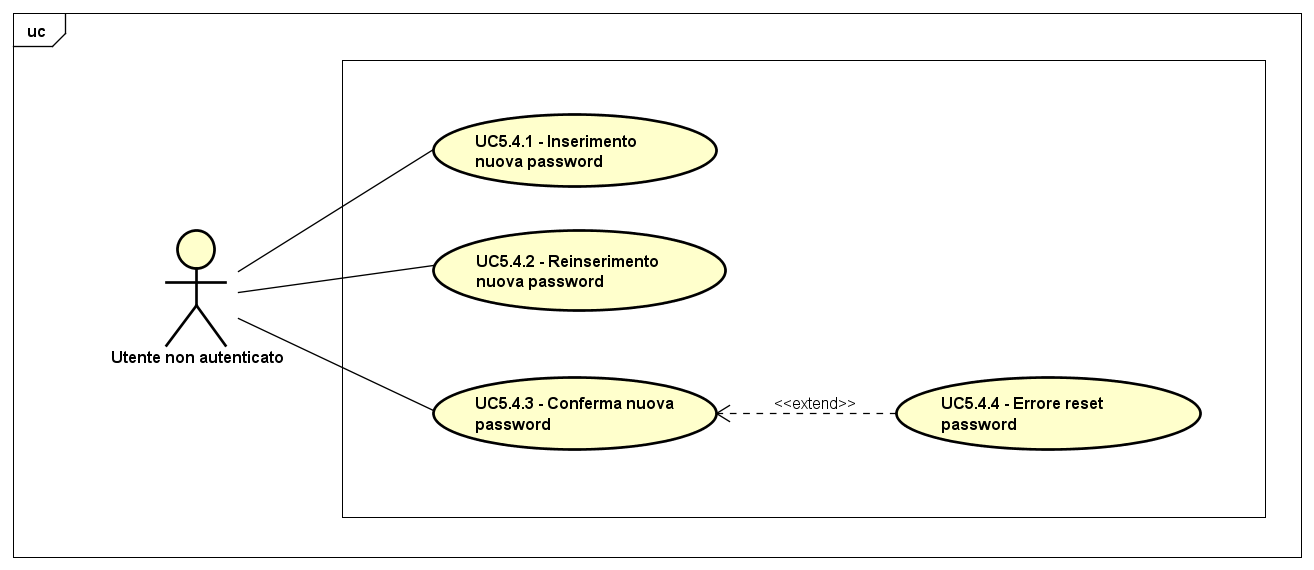
\includegraphics[scale=0.45]{UML/UC5_4.png}
	\caption{UC5.4: Reset password}
\end{figure}

\begin{minipage}{\linewidth}
	\begin{longtable}{ l | p{11cm}}
		\hline
		\rowcolor{Gray}
		\multicolumn{2}{c}{UC5.4 - Reset password} \\
		\hline
		\textbf{Attori} & Utente non autenticato \\
		\textbf{Descrizione} & L'attore ha ricevuto un link per la schermata di reset della propria password \\
		\textbf{Pre-Condizioni} & L'attore ha richiesto il recupero della password ed ha aperto il link per poterla resettare \\
		\textbf{Post-Condizioni} & L'attore ha resettato con successo la password \\
		\textbf{Scenario Principale} & 
		\begin{enumerate*}[label=(\arabic*.),itemjoin={\newline}]
			\item L'attore può inserire la nuova password desiderata (UC5.4.1)
			\item L'attore può reinserire la nuova password desiderata (UC5.4.2)
			\item L'attore può confermare i dati inseriti e completare la procedura con successo (UC5.4.3)
		\end{enumerate*}\\
		\textbf{Scenari Alternativi} & 
		\begin{enumerate*}[label=(\arabic*.),itemjoin={\newline}]
			\item L'attore visualizza un errore qualora le password inserite non coincidano o i campi risultino vuoti (UC5.4.4)
		\end{enumerate*}\\
	\end{longtable}
\end{minipage}

\paragraph{Caso d'uso UC5.4.1: Inserimento nuova password}
\label{UC5_4_1}

\begin{minipage}{\linewidth}
	\begin{longtable}{ l | p{11cm}}
		\hline
		\rowcolor{Gray}
		\multicolumn{2}{c}{UC5.4.1 - Inserimento nuova password} \\
		\hline
		\textbf{Attori} & Utente non autenticato \\
		\textbf{Descrizione} & L'attore inserisce la nuova password per il proprio account \\
		\textbf{Pre-Condizioni} & L'applicazione mostra la schermata di reset password \\
		\textbf{Post-Condizioni} & L'attore ha inserito la nuova password \\
		\textbf{Scenario Principale} & 
		\begin{enumerate*}[label=(\arabic*.),itemjoin={\newline}]
			\item L'attore può inserire la nuova password per il proprio account
		\end{enumerate*}\\
	\end{longtable}
\end{minipage}

\paragraph{Caso d'uso UC5.4.2: Reinserimento nuova password}
\label{UC5_4_2}

\begin{minipage}{\linewidth}
	\begin{longtable}{ l | p{11cm}}
		\hline
		\rowcolor{Gray}
		\multicolumn{2}{c}{UC5.4.2 - Reinserimento nuova password} \\
		\hline
		\textbf{Attori} & Utente non autenticato \\
		\textbf{Descrizione} & L'attore reinserisce la nuova password per il proprio account \\
		\textbf{Pre-Condizioni} & L'applicazione mostra la schermata di reset password \\
		\textbf{Post-Condizioni} & L'attore ha reinserito la nuova password \\
		\textbf{Scenario Principale} & 
		\begin{enumerate*}[label=(\arabic*.),itemjoin={\newline}]
			\item L'attore può reinserire la nuova password per il proprio account
		\end{enumerate*}\\
	\end{longtable}
\end{minipage}

\paragraph{Caso d'uso UC5.4.3: Conferma nuova password}
\label{UC5_4_3}

\begin{minipage}{\linewidth}
	\begin{longtable}{ l | p{11cm}}
		\hline
		\rowcolor{Gray}
		\multicolumn{2}{c}{UC5.4.3 - Conferma nuova password} \\
		\hline
		\textbf{Attori} & Utente non autenticato \\
		\textbf{Descrizione} & L'attore conferma i dati inseriti per poter resettare la propria password \\
		\textbf{Pre-Condizioni} & L'applicazione mostra la schermata di reset password \\
		\textbf{Post-Condizioni} & L'attore ha confermato i nuovi dati per il proprio account \\
		\textbf{Scenario Principale} & 
		\begin{enumerate*}[label=(\arabic*.),itemjoin={\newline}]
			\item L'attore può confermare i nuovi dati per il proprio account, visualizzando un messaggio di successo e venendo reindirizzato alla schermata principale (UC1)
		\end{enumerate*}\\
	\end{longtable}
\end{minipage}

\paragraph{Caso d'uso UC5.4.4: Errore reset password}
\label{UC5_4_4}

\begin{minipage}{\linewidth}
	\begin{longtable}{ l | p{11cm}}
		\hline
		\rowcolor{Gray}
		\multicolumn{2}{c}{UC5.4.4 - Errore reset password} \\
		\hline
		\textbf{Attori} & Utente non autenticato \\
		\textbf{Descrizione} & L'attore conferma i dati inseriti per poter resettare la propria password \\
		\textbf{Pre-Condizioni} & L'attore ha confermato i dati inseriti per poter resettare la propria password \\
		\textbf{Post-Condizioni} & L'attore non ha confermato con successo i propri nuovi dati di accesso \\
		\textbf{Scenario Principale} & 
		\begin{enumerate*}[label=(\arabic*.),itemjoin={\newline}]
			\item L'attore visualizza un messaggio di errore poiché le password non coincidono o i campi sono vuoti
		\end{enumerate*}\\
	\end{longtable}
\end{minipage}
\newpage
\subsection{Caso d'uso UC6: Ricerca API}
\label{UC6}
\begin{figure}[ht]
	\centering
	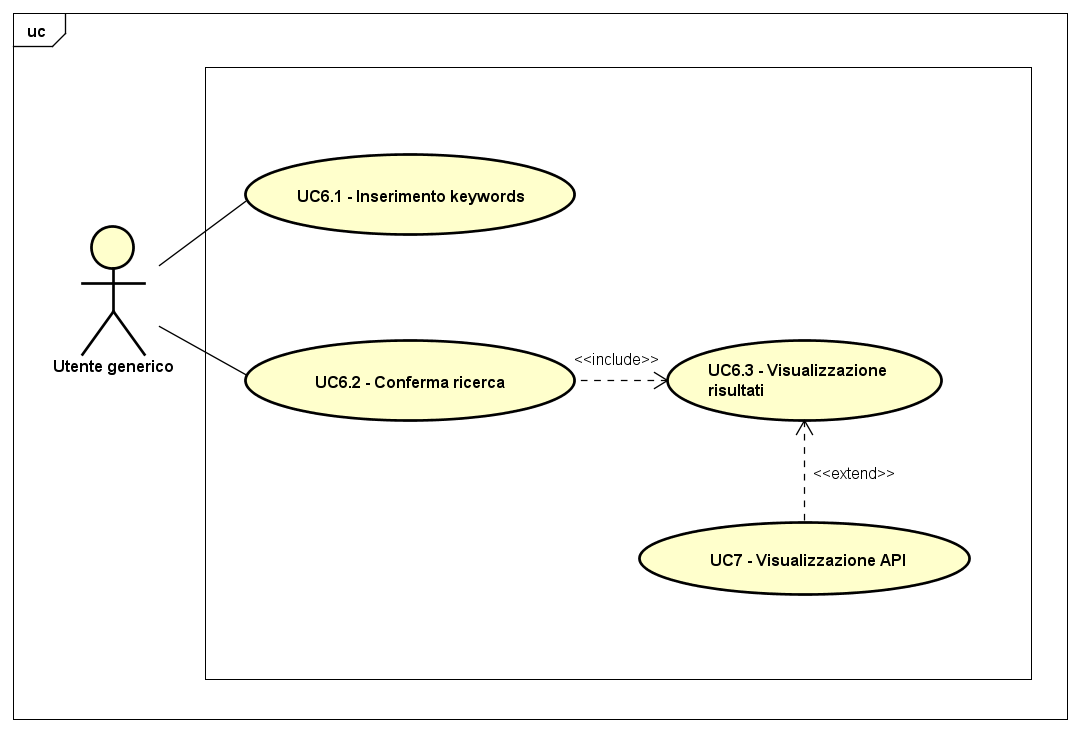
\includegraphics[scale=0.45]{UML/UC6.png}
	\caption{UC6: Ricerca API}
\end{figure}

\begin{longtable}{ l | p{11cm}}
	\hline
	\rowcolor{Gray}
	 \multicolumn{2}{c}{UC6 - Ricerca API} \\
	 \hline
	\textbf{Attori} & Utente generico, Utente non autenticato, Utente autenticato, Amministratore API Market \\
	\textbf{Descrizione} & L'attore inserisce le keywords per la ricerca di API \\
	\textbf{Pre-Condizioni} & L'attore ha scelto di effettuare una ricerca di API \\
	\textbf{Post-Condizioni} & L'attore ha effettuato la ricerca di API ed ha visualizzato la lista dei risultati \\
	\textbf{Scenario Principale} & 
	\begin{enumerate*}[label=(\arabic*.),itemjoin={\newline}]
		\item L'attore può inserire la stringa di ricerca desiderata (UC6.1)
		\item L'attore può confermare i dati inseriti (UC6.2) e visualizzare i risultati forniti dall'applicazione web (UC6.3)
	\end{enumerate*}\\
\end{longtable}
\subsubsection{Caso d'uso UC6.1: Inserimento keywords}
\label{UC6_1}

\begin{minipage}{\linewidth}
\begin{tabular}{ l | p{11cm}}
	\hline
	\rowcolor{Gray}
	 \multicolumn{2}{c}{UC6.1 - Inserimento keywords} \\
	 \hline
	\textbf{Attori} & Utente generico, Utente non autenticato, Utente autenticato, Amministratore API Market \\
	\textbf{Descrizione} & L'attore effettua una ricerca delle API inserendo nella barra di ricerca una stringa contenente le keywords desiderate \\
	\textbf{Pre-Condizioni} & L'attore ha scelto di effettuare una ricerca di API \\
	\textbf{Post-Condizioni} & L'attore ha inserito nella barra di ricerca una stringa contenente le keywords desiderate \\
	\textbf{Scenario Principale} & 
	\begin{enumerate*}[label=(\arabic*.),itemjoin={\newline}]
		\item L'attore può inserire nella barra di ricerca una stringa con tenente le keywords desiderate: esse verranno ricercate sul nome dell'API, sul nome dell'autore e su eventuali tag
	\end{enumerate*}\\
\end{tabular}
\end{minipage}
\subsubsection{Caso d'uso UC6.2: Conferma ricerca}
\label{UC6_2}

\begin{minipage}{\linewidth}
	\begin{tabular}{ l | p{11cm}}
		\hline
		\rowcolor{Gray}
		\multicolumn{2}{c}{UC6.2 - Conferma ricerca} \\
		\hline
		\textbf{Attori} & Utente generico, Utente non autenticato, Utente autenticato, Amministratore API Market \\
		\textbf{Descrizione} & L'attore conferma la stringa di ricerca inserita per poter visualizzare i risultati \\
		\textbf{Pre-Condizioni} & L'attore ha inserito una stringa di ricerca \\
		\textbf{Post-Condizioni} & L'attore ha confermato una stringa di ricerca \\
		\textbf{Scenario Principale} & 
		\begin{enumerate*}[label=(\arabic*.),itemjoin={\newline}]
			\item L'attore può confermare una stringa di ricerca, visualizzando la lista dei risultati (UC6.3)
		\end{enumerate*}\\
	\end{tabular}
\end{minipage}
\subsubsection{Caso d'uso UC6.3: Visualizzazione risultati}
\label{UC6_3}

\begin{minipage}{\linewidth}
	\begin{tabular}{ l | p{11cm}}
		\hline
		\rowcolor{Gray}
		\multicolumn{2}{c}{UC6.3 - Visualizzazione risultati} \\
		\hline
		\textbf{Attori} & Utente generico, Utente non autenticato, Utente autenticato, Amministratore API Market \\
		\textbf{Descrizione} & L'attore visualizza le API che corrispondono alle keywords della ricerca effettuata \\
		\textbf{Pre-Condizioni} & L'attore ha confermato la ricerca API \\
		\textbf{Post-Condizioni} & L'attore ha visualizzato le API che corrispondono alle keywords della ricerca effettuata \\
		\textbf{Scenario Principale} & 
		\begin{enumerate*}[label=(\arabic*.),itemjoin={\newline}]
			\item L'attore può visualizzare le API che corrispondono alle keywords della ricerca effettuata, che possono essere anche vuoti nel caso di stringhe non consone
		\end{enumerate*}\\
		\textbf{Scenari Alternativi} & 
		\begin{enumerate*}[label=(\arabic*.),itemjoin={\newline}]
		\item L'attore può accedere alla schermata delle singole API tramite la lista delle API (UC7)
	\end{enumerate*}\\
	\end{tabular}
\end{minipage}
\newpage
\subsection{Caso d'uso UC7: Visualizzazione API}
\label{UC7}
\begin{figure}[ht]
	\centering
	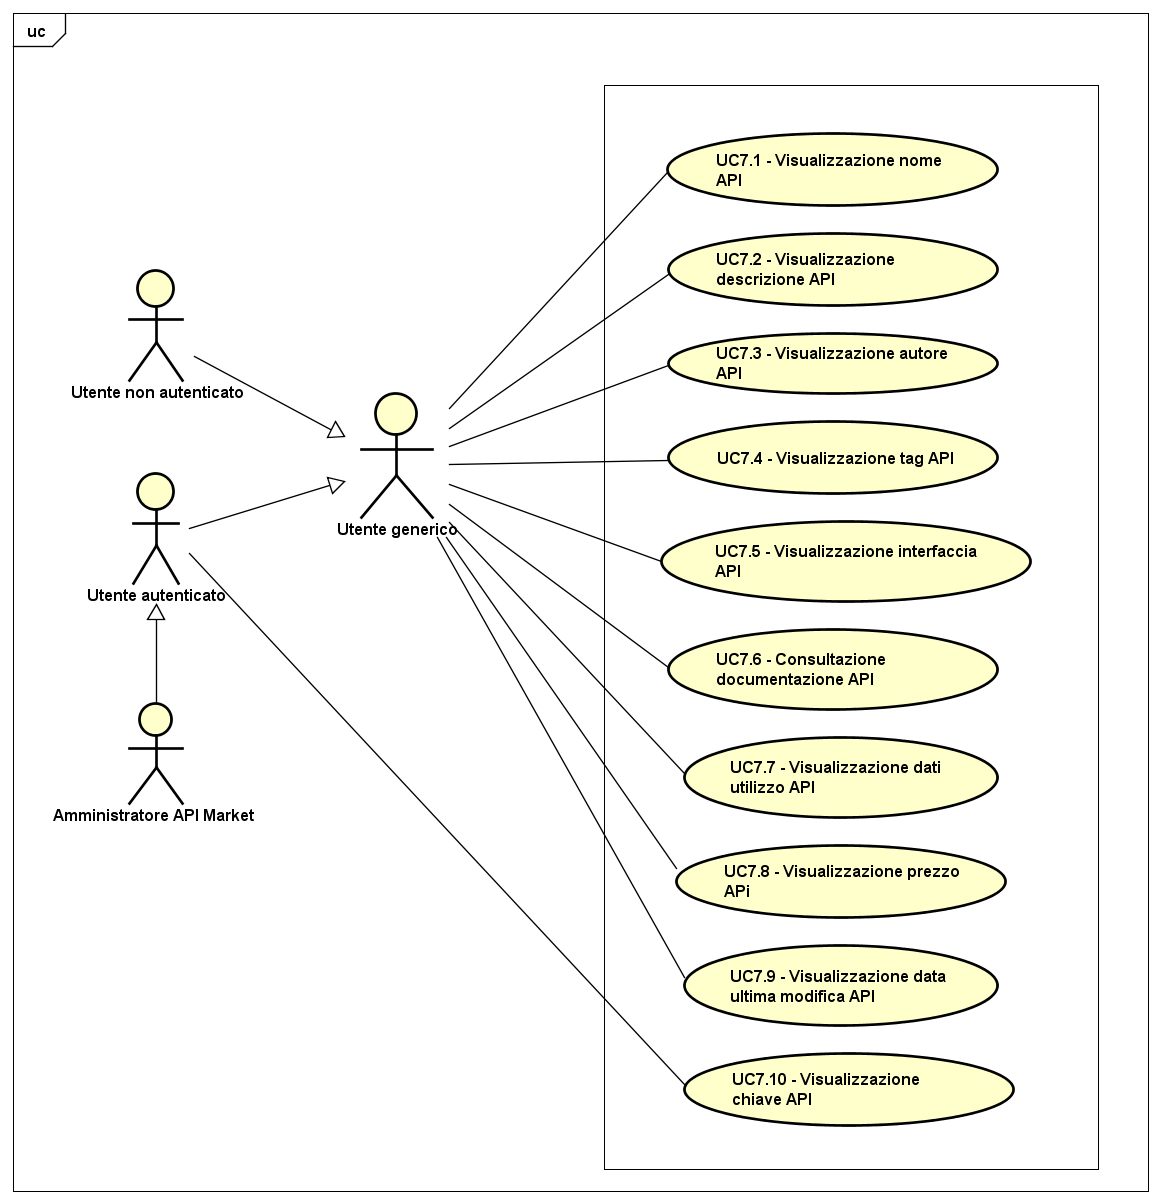
\includegraphics[scale=0.45]{UML/UC7.png}
	\caption{UC7: Visualizzazione API}
\end{figure}

\begin{longtable}{ l | p{11cm}}
	\hline
	\rowcolor{Gray}
	\multicolumn{2}{c}{UC7 - Visualizzazione API}\\
	\hline
	
	 \textbf{Attori} & Utente generico \\
	\textbf{Descrizione} & L'attore visualizza i dati relativi ad una API \\
	\textbf{Pre-Condizioni} & L'attore ha selezionato una API tramite un link (E.g: Ottenuto da una ricerca) \\
	\textbf{Post-Condizioni} & L'attore ha visualizzato i dati relativi all'API selezionata \\
	\textbf{Scenario Principale} &
	\begin{enumerate*}[label=(\arabic*.),itemjoin={\newline}]
		\item L'attore può visualizzare il nome dell'API (UC7.1)
		\item L'attore può visualizzare la descrizione dell'API (UC7.2)
		\item L'attore può visualizzare il nome dell'autore dell'API (UC7.3)
		\item L'attore può visualizzare la categoria dell'API (UC7.4)
		\item L'attore può visualizzare l'interfaccia dell'API (UC7.5)
		\item L'attore può consultare la documentazione dell'API (UC7.6)
		\item L'attore può visualizzare i dati di utilizzo dell'API (UC7.7)
		\item L'attore può visualizzare il prezzo dell'API (UC7.8)
		\item L'attore può visualizzare la data dell'ultima modifica all'API (UC7.9)
		\item L'attore può visualizzare la versione dell'API (UC7.10)
		\item L'attore può visualizzare il logo dell'API (UC7.11)
		\item L'attore può visualizzare la policy di vendita dell'API (UC7.12)
		\item L'attore può visualizzare il link alla pagine d'acquisto dell'API (UC7.13)
	\end{enumerate*}\\
\end{longtable}


\subsubsection{Caso d'uso UC7.1: Visualizzazione nome API}
\label{UC7_1}

\begin{minipage}{\linewidth}
	\begin{tabular}{ l | p{11cm}}
		\hline
		\rowcolor{Gray}
		\multicolumn{2}{c}{UC7.1 - Visualizzazione nome API} \\
		\hline
		\textbf{Attori} & Utente generico \\
		\textbf{Descrizione} & L'attore visualizza nella schermata relativa il nome dell'API \\
		\textbf{Pre-Condizioni} & L'attore si trova nella schermata di visualizzazione API dell'API precedentemente selezionata \\
		\textbf{Post-Condizioni} & L'attore ha visualizzato il nome dell'API selezionata \\
		\textbf{Scenario Principale} & 
		\begin{enumerate*}[label=(\arabic*.),itemjoin={\newline}]
			\item L'attore può visualizzare il nome dell'API selezionata
		\end{enumerate*}\\
	\end{tabular}
\end{minipage}

\subsubsection{Caso d'uso UC7.2: Visualizzazione descrizione API}
\label{UC7_2}

\begin{minipage}{\linewidth}
	\begin{tabular}{ l | p{11cm}}
		\hline
		\rowcolor{Gray}
		\multicolumn{2}{c}{UC7.2 - Visualizzazione descrizione API} \\
		\hline
		\textbf{Attori} & Utente generico \\
		\textbf{Descrizione} & L'attore visualizza nella schermata relativa la descrizione dell'API \\
		\textbf{Pre-Condizioni} & L'attore si trova nella schermata di visualizzazione API dell'API precedentemente selezionata \\
		\textbf{Post-Condizioni} & L'attore ha visualizzato la descrizione dell'API selezionata \\
		\textbf{Scenario Principale} & 
		\begin{enumerate*}[label=(\arabic*.),itemjoin={\newline}]
			\item L'attore può visualizzare la descrizione dell'API selezionata
		\end{enumerate*}\\
	\end{tabular}
\end{minipage}

\subsubsection{Caso d'uso UC7.3: Visualizzazione autore API}
\label{UC7_3}

\begin{minipage}{\linewidth}
	\begin{tabular}{ l | p{11cm}}
		\hline
		\rowcolor{Gray}
		\multicolumn{2}{c}{UC7.3 - Visualizzazione autore API} \\
		\hline
		\textbf{Attori} & Utente generico \\
		\textbf{Descrizione} & L'attore visualizza nella schermata relativa il nome dell'autore dell'API \\
		\textbf{Pre-Condizioni} & L'attore si trova nella schermata di visualizzazione API dell'API precedentemente selezionata \\
		\textbf{Post-Condizioni} & L'attore ha visualizzato il nome dell'autore per l'API selezionata \\
		\textbf{Scenario Principale} & 
		\begin{enumerate*}[label=(\arabic*.),itemjoin={\newline}]
			\item L'attore può visualizzare il nome dell'autore per l'API selezionata
		\end{enumerate*}\\
	\end{tabular}
\end{minipage}

\subsubsection{Caso d'uso UC7.4: Visualizzazione categoria API}
\label{UC7_4}

\begin{minipage}{\linewidth}
	\begin{tabular}{ l | p{11cm}}
		\hline
		\rowcolor{Gray}
		\multicolumn{2}{c}{UC7.4 - Visualizzazione categoria API} \\
		\hline
		\textbf{Attori} & Utente generico \\
		\textbf{Descrizione} & L'attore visualizza nella schermata relativa la categoria dell'API \\
		\textbf{Pre-Condizioni} & L'attore si trova nella schermata di visualizzazione API dell'API precedentemente selezionata \\
		\textbf{Post-Condizioni} & L'attore ha visualizzato la categoria dell'API selezionata \\
		\textbf{Scenario Principale} & 
		\begin{enumerate*}[label=(\arabic*.),itemjoin={\newline}]
			\item L'attore può visualizzare la categoria dell'API selezionata
		\end{enumerate*}\\
	\end{tabular}
\end{minipage}

\newpage
\subsubsection{Caso d'uso UC7.5: Visualizzazione interfaccia API}
\label{UC7_5}
\begin{figure}[ht]
	\centering
	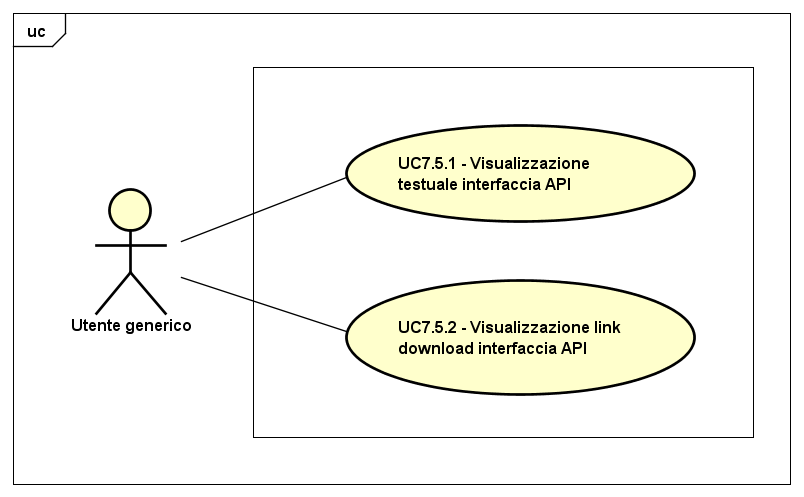
\includegraphics[scale=0.45]{UML/UC7_5.png}
	\caption{UC7.5: Visualizzazione interfaccia API}
\end{figure}

\begin{minipage}{\linewidth}
	\begin{tabular}{ l | p{11cm}}
		\hline
		\rowcolor{Gray}
		\multicolumn{2}{c}{UC7.5 - Visualizzazione interfaccia API} \\
		\hline
		\textbf{Attori} & Utente generico \\
		\textbf{Descrizione} & L'attore visualizza nella schermata relativa l'interfaccia dell'API \\
		\textbf{Pre-Condizioni} & L'attore si trova nella schermata di visualizzazione API dell'API precedentemente selezionata \\
		\textbf{Post-Condizioni} & L'attore ha visualizzato l'interfaccia dell'API selezionata \\
		\textbf{Scenario Principale} & 
		\begin{enumerate*}[label=(\arabic*.),itemjoin={\newline}]
			\item L'attore può visualizzare testualmente l'interfaccia dell'API selezionata (UC7.5.1)
			\item L'attore può visualizzare il link di download dell'interfaccia dell'API selezionata (UC7.5.2)
		\end{enumerate*}\\
	\end{tabular}
\end{minipage}

\paragraph{Caso d'uso UC7.5.1: Visualizzazione testuale interfaccia API}
\label{UC7_5_1}

\begin{minipage}{\linewidth}
	\begin{tabular}{ l | p{11cm}}
		\hline
		\rowcolor{Gray}
		\multicolumn{2}{c}{UC7.5.1 - Visualizzazione testuale interfaccia API} \\
		\hline
		\textbf{Attori} & Utente generico \\
		\textbf{Descrizione} & L'attore visualizza testualmente l'interfaccia dell'API \\
		\textbf{Pre-Condizioni} & L'attore si trova nella schermata di visualizzazione API dell'API precedentemente selezionata \\
		\textbf{Post-Condizioni} & L'attore ha visualizzato testualmente l'interfaccia dell'API selezionata \\
		\textbf{Scenario Principale} & 
		\begin{enumerate*}[label=(\arabic*.),itemjoin={\newline}]
			\item L'attore può visualizzare testualmente l'interfaccia dell'API selezionata
		\end{enumerate*}\\
	\end{tabular}
\end{minipage}

\paragraph{Caso d'uso UC7.5.2: Visualizzazione link download interfaccia API}
\label{UC7_5_2}

\begin{minipage}{\linewidth}
	\begin{tabular}{ l | p{11cm}}
		\hline
		\rowcolor{Gray}
		\multicolumn{2}{c}{UC7.5.2 - Visualizzazione link download interfaccia API} \\
		\hline
		\textbf{Attori} & Utente generico \\
		\textbf{Descrizione} & L'attore visualizza il link di download dell'interfaccia dell'API \\
		\textbf{Pre-Condizioni} & L'attore si trova nella schermata di visualizzazione API dell'API precedentemente selezionata \\
		\textbf{Post-Condizioni} & L'attore ha visualizzato il link di download dell'interfaccia dell'API selezionata \\
		\textbf{Scenario Principale} & 
		\begin{enumerate*}[label=(\arabic*.),itemjoin={\newline}]
			\item L'attore può visualizzare il link di download dell'interfaccia dell'API selezionata
		\end{enumerate*}\\
	\end{tabular}
\end{minipage}

\newpage
\subsubsection{Caso d'uso UC7.6: Consultazione documentazione API}
\label{UC7_6}
\begin{figure}[ht]
	\centering
	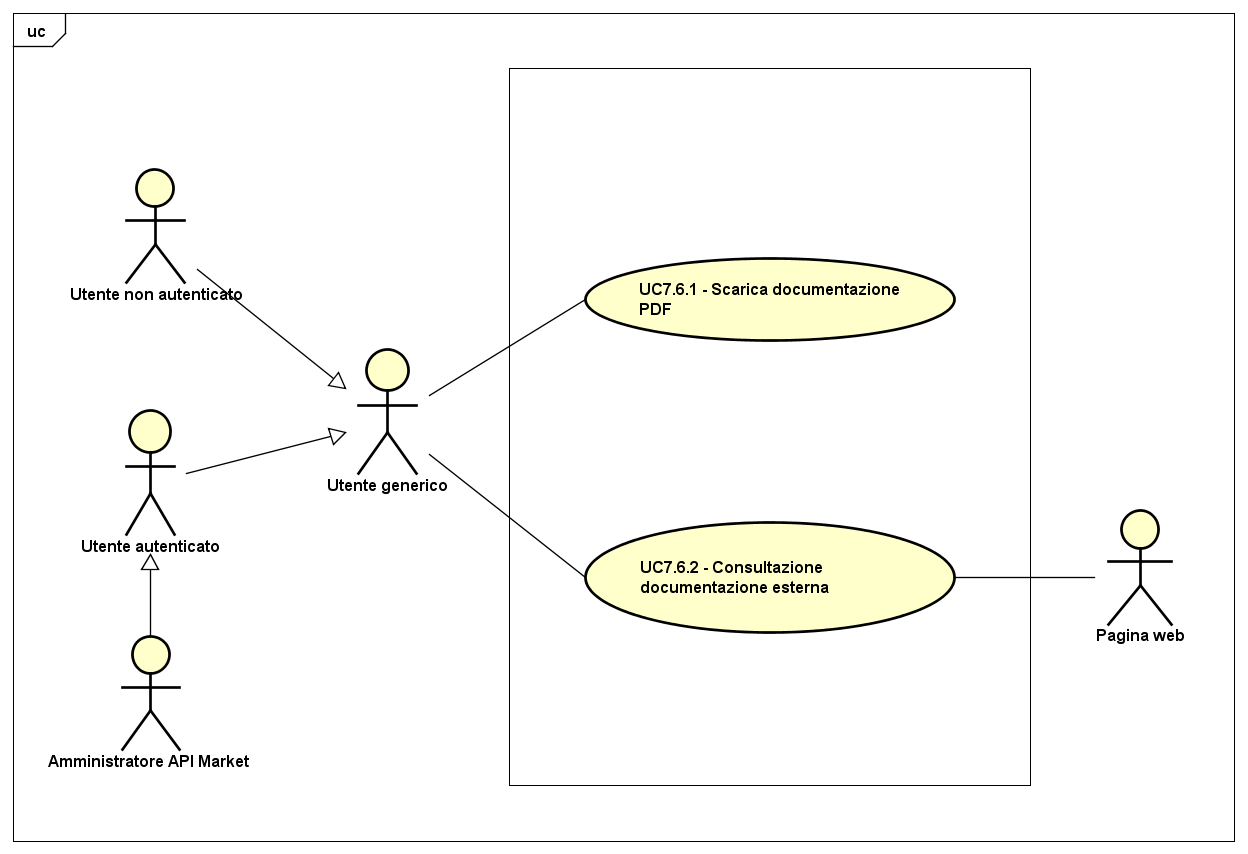
\includegraphics[scale=0.45]{UML/UC7_6.png}
	\caption{UC7.6: Visualizzazione API}
\end{figure}

\begin{minipage}{\linewidth}
	\begin{tabular}{ l | p{11cm}}
		\hline
		\rowcolor{Gray}
		\multicolumn{2}{c}{UC7.6 - Consultazione documentazione API} \\
		\hline
		\textbf{Attori} & Utente generico \\
		\textbf{Descrizione} & L'attore consulta la documentazione dell'API \\
		\textbf{Pre-Condizioni} & L'attore si trova nella schermata di visualizzazione API dell'API precedentemente selezionata \\
		\textbf{Post-Condizioni} & L'attore ha consultato la documentazione dell'API selezionata \\
		\textbf{Scenario Principale} & 
		\begin{enumerate*}[label=(\arabic*.),itemjoin={\newline}]
			\item L'attore può consultare la documentazione dell'API selezionata scaricando il file PDF fornito dall'autore (UC7.6.1)
			\item L'attore può consultare la documentazione dell'API selezionata tramite un link esterno fornita dall'autore (UC7.6.2)
		\end{enumerate*}\\
	\end{tabular}
\end{minipage}

\paragraph{Caso d'uso UC7.6.1: Scarica documentazione PDF}
\label{UC7_6_1}

\begin{minipage}{\linewidth}
	\begin{tabular}{ l | p{11cm}}
		\hline
		\rowcolor{Gray}
		\multicolumn{2}{c}{UC7.6.1 - Scarica documentazione PDF} \\
		\hline
		\textbf{Attori} & Utente generico \\
		\textbf{Descrizione} & L'attore scarica la documentazione dell'API in formato PDF tramite un link \\
		\textbf{Pre-Condizioni} & L'attore si trova nella schermata relativa alla consultazione della documentazione dell'API \\
		\textbf{Post-Condizioni} & L'attore ha scaricato la documentazione dell'API in formato PDF \\
		\textbf{Scenario Principale} & 
		\begin{enumerate*}[label=(\arabic*.),itemjoin={\newline}]
			\item L'attore può scaricare la documentazione dell'API in formato PDF
		\end{enumerate*}\\
	\end{tabular}
\end{minipage}

\paragraph{Caso d'uso UC7.6.2: Consultazione documentazione esterna}
\label{UC7_6_2}

\begin{minipage}{\linewidth}
	\begin{tabular}{ l | p{11cm}}
		\hline
		\rowcolor{Gray}
		\multicolumn{2}{c}{UC7.6.2 - Consultazione documentazione esterna} \\
		\hline
		\textbf{Attori} & Utente generico, Pagina web \\
		\textbf{Descrizione} & L'attore consulta la documentazione dell'API tramite un link esterno fornito dall'autore \\
		\textbf{Pre-Condizioni} & L'attore si trova nella schermata relativa alla consultazione della documentazione dell'API \\
		\textbf{Post-Condizioni} & L'attore ha aperto il link alla documentazione esterna dell'API ed è stato reindirizzato ad una pagina esterna specificata dall'autore dell'API \\
		\textbf{Scenario Principale} & 
		\begin{enumerate*}[label=(\arabic*.),itemjoin={\newline}]
			\item L'attore può consultare la documentazione esterna dell'API aprendo il link ad una pagina esterna specificata dall'autore dell'API
		\end{enumerate*}\\
	\end{tabular}
\end{minipage}

\newpage
\subsubsection{Caso d'uso UC7.7: Visualizzazione dati di utilizzo API}
\label{UC7_7}
\begin{figure}[ht]
	\centering
	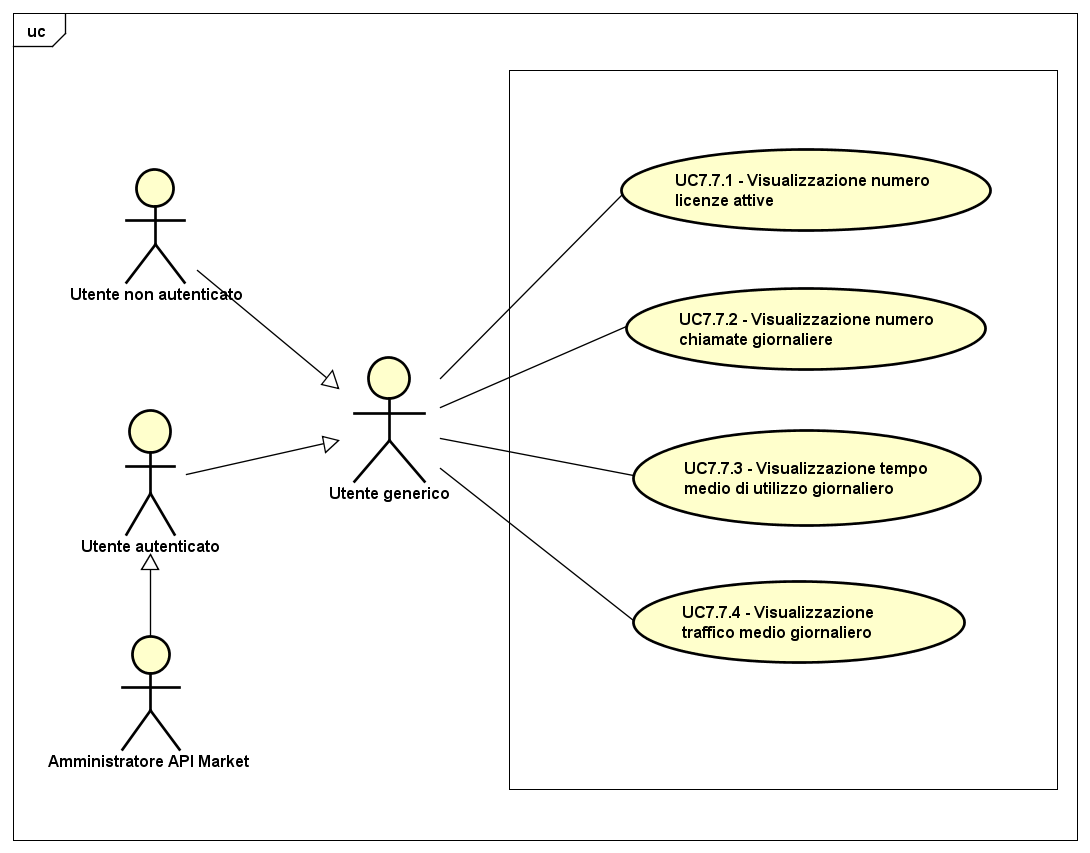
\includegraphics[scale=0.45]{UML/UC7_7.png}
	\caption{UC7.7: Visualizzazione API}
\end{figure}

\begin{minipage}{\linewidth}
	\begin{tabular}{ l | p{11cm}}
		\hline
		\rowcolor{Gray}
		\multicolumn{2}{c}{UC7.7 - Visualizzazione dati di utilizzo API} \\
		\hline
		\textbf{Attori} & Utente generico \\
		\textbf{Descrizione} & L'attore visualizza nella schermata relativa i dati di utilizzo dell'API \\
		\textbf{Pre-Condizioni} & L'attore si trova nella schermata di visualizzazione API dell'API precedentemente selezionata \\
		\textbf{Post-Condizioni} & L'attore ha visualizzato i dati di utilizzo dell'API selezionata \\
		\textbf{Scenario Principale} & 
		\begin{enumerate*}[label=(\arabic*.),itemjoin={\newline}]
			\item L'attore può visualizzare il numero di licenze attive per l'API selezionata (UC7.7.1)
			\item L'attore può visualizzare i dati di SLA dell'API selezionata (UC7.7.2)
		\end{enumerate*}\\
	\end{tabular}
\end{minipage}

\paragraph{Caso d'uso UC7.7.1: Visualizzazione numero licenze attive}
\label{UC7_7_1}

\begin{minipage}{\linewidth}
	\begin{tabular}{ l | p{11cm}}
		\hline
		\rowcolor{Gray}
		\multicolumn{2}{c}{UC7.7.1 - Visualizzazione numero licenze attive} \\
		\hline
		\textbf{Attori} & Utente generico \\
		\textbf{Descrizione} & L'attore visualizza il numero di licenze attive per l'API selezionata \\
		\textbf{Pre-Condizioni} & L'attore si trova nella schermata di visualizzazione dati di utilizzo API \\
		\textbf{Post-Condizioni} & L'attore ha visualizzato il numero di licenze attive per l'API selezionata \\
		\textbf{Scenario Principale} & 
		\begin{enumerate*}[label=(\arabic*.),itemjoin={\newline}]
			\item L'attore può visualizzare il numero di licenze attive per l'API selezionata
		\end{enumerate*}\\
	\end{tabular}
\end{minipage}

\paragraph{Caso d'uso UC7.7.2: Visualizzazione dati SLA}
\label{UC7_7_2}

\begin{minipage}{\linewidth}
	\begin{tabular}{ l | p{11cm}}
		\hline
		\rowcolor{Gray}
		\multicolumn{2}{c}{UC7.7.2 - Visualizzazione dati SLA} \\
		\hline
		\textbf{Attori} & Utente generico \\
		\textbf{Descrizione} & L'attore visualizza  all'API selezionata \\
		\textbf{Pre-Condizioni} & L'attore si trova nella schermata di visualizzazione dati di utilizzo API \\
		\textbf{Post-Condizioni} & L'attore ha visualizzato i dati di SLA dell'API selezionata \\
		\textbf{Scenario Principale} & 
		\begin{enumerate*}[label=(\arabic*.),itemjoin={\newline}]
			\item L'attore può visualizzare i dati di SLA dell'API selezionata
		\end{enumerate*}\\
	\end{tabular}
\end{minipage}

\subsubsection{Caso d'uso UC7.8: Visualizzazione prezzo API}
\label{UC7_8}

\begin{minipage}{\linewidth}
	\begin{tabular}{ l | p{11cm}}
		\hline
		\rowcolor{Gray}
		\multicolumn{2}{c}{UC7.8 - Visualizzazione prezzo API} \\
		\hline
		\textbf{Attori} & Utente generico \\
		\textbf{Descrizione} & L'attore visualizza nella schermata relativa il prezzo dell'API \\
		\textbf{Pre-Condizioni} & L'attore si trova nella schermata di visualizzazione API dell'API precedentemente selezonata \\
		\textbf{Post-Condizioni} & L'attore ha visualizzato il prezzo dell'API selezionata \\
		\textbf{Scenario Principale} & 
		\begin{enumerate*}[label=(\arabic*.),itemjoin={\newline}]
			\item L'attore può visualizzare il prezzo dell'API (secondo la policy stabilita dall'autore)
		\end{enumerate*}\\
	\end{tabular}
\end{minipage}

\subsubsection{Caso d'uso UC7.9: Visualizzazione data ultima modifica API}
\label{UC7_9}

\begin{minipage}{\linewidth}
	\begin{tabular}{ l | p{11cm}}
		\hline
		\rowcolor{Gray}
		\multicolumn{2}{c}{UC7.9 - Visualizzazione data ultima modifica API} \\
		\hline
		\textbf{Attori} & Utente generico \\
		\textbf{Descrizione} & L'attore visualizza nella schermata relativa la data dell'ultima modifica effettuata sull'API \\
		\textbf{Pre-Condizioni} & L'attore ha selezionato una API, ne possiede la licenza attiva e si trova nella schermata di visualizzazione API \\
		\textbf{Post-Condizioni} & L'attore ha visualizzato nella schermata relativa la data dell'ultima modifica effettuata sull'API selezionata \\
		\textbf{Scenario Principale} & 
		\begin{enumerate*}[label=(\arabic*.),itemjoin={\newline}]
			\item L'attore può visualizzare nella schermata relativa la data dell'ultima modifica effettuata sull'API selezionata
		\end{enumerate*}\\
	\end{tabular}
\end{minipage}

\subsubsection{Caso d'uso UC7.10: Visualizzazione versione API}
\label{UC7_10}

\begin{minipage}{\linewidth}
	\begin{tabular}{ l | p{11cm}}
		\hline
		\rowcolor{Gray}
		\multicolumn{2}{c}{UC7.10 - Visualizzazione versione API} \\
		\hline
		\textbf{Attori} & Utente generico \\
		\textbf{Descrizione} & L'attore visualizza nella schermata relativa la versione dell'API \\
		\textbf{Pre-Condizioni} & L'attore si trova nella schermata di visualizzazione API dell'API precedentemente selezonata \\
		\textbf{Post-Condizioni} & L'attore ha visualizzato la versione dell'API selezionata \\
		\textbf{Scenario Principale} & 
		\begin{enumerate*}[label=(\arabic*.),itemjoin={\newline}]
			\item L'attore può visualizzare la versione dell'API
		\end{enumerate*}\\
	\end{tabular}
\end{minipage}

\subsubsection{Caso d'uso UC7.11: Visualizzazione logo API}
\label{UC7_11}

\begin{minipage}{\linewidth}
	\begin{tabular}{ l | p{11cm}}
		\hline
		\rowcolor{Gray}
		\multicolumn{2}{c}{UC7.11 - Visualizzazione logo API} \\
		\hline
		\textbf{Attori} & Utente generico \\
		\textbf{Descrizione} & L'attore visualizza nella schermata relativa il logo dell'API \\
		\textbf{Pre-Condizioni} & L'attore si trova nella schermata di visualizzazione API dell'API precedentemente selezonata \\
		\textbf{Post-Condizioni} & L'attore ha visualizzato il logo dell'API selezionata \\
		\textbf{Scenario Principale} & 
		\begin{enumerate*}[label=(\arabic*.),itemjoin={\newline}]
			\item L'attore può visualizzare il logo dell'API
		\end{enumerate*}\\
	\end{tabular}
\end{minipage}

\subsubsection{Caso d'uso UC7.12: Visualizzazione policy vendita API}
\label{UC7_12}

\begin{minipage}{\linewidth}
	\begin{tabular}{ l | p{11cm}}
		\hline
		\rowcolor{Gray}
		\multicolumn{2}{c}{UC7.12 - Visualizzazione policy vendita API} \\
		\hline
		\textbf{Attori} & Utente generico \\
		\textbf{Descrizione} & L'attore visualizza nella schermata relativa la policy di vendita dell'API \\
		\textbf{Pre-Condizioni} & L'attore si trova nella schermata di visualizzazione API dell'API precedentemente selezonata \\
		\textbf{Post-Condizioni} & L'attore ha visualizzato la policy di vendita dell'API selezionata \\
		\textbf{Scenario Principale} & 
		\begin{enumerate*}[label=(\arabic*.),itemjoin={\newline}]
			\item L'attore può visualizzare la policy di vendita dell'API
		\end{enumerate*}\\
	\end{tabular}
\end{minipage}

\subsubsection{Caso d'uso UC7.13: Visualizzazione link acquisto API}
\label{UC7_13}

\begin{minipage}{\linewidth}
	\begin{tabular}{ l | p{11cm}}
		\hline
		\rowcolor{Gray}
		\multicolumn{2}{c}{UC7.13 - Visualizzazione link acquisto API} \\
		\hline
		\textbf{Attori} & Utente generico \\
		\textbf{Descrizione} & L'attore visualizza nella schermata relativa il link alla pagina d'acquisto dell'API \\
		\textbf{Pre-Condizioni} & L'attore si trova nella schermata di visualizzazione API dell'API precedentemente selezonata \\
		\textbf{Post-Condizioni} & L'attore ha visualizzato il link alla pagina d'acquisto dell'API selezionata \\
		\textbf{Scenario Principale} & 
		\begin{enumerate*}[label=(\arabic*.),itemjoin={\newline}]
			\item L'attore può visualizzare il link alla pagina d'acquisto dell'API
		\end{enumerate*}\\
	\end{tabular}
\end{minipage}
\newpage
\subsection{Caso d'uso UC8: Visualizzazione API acquistate}
\label{UC8}
\begin{figure}[ht]
	\centering
	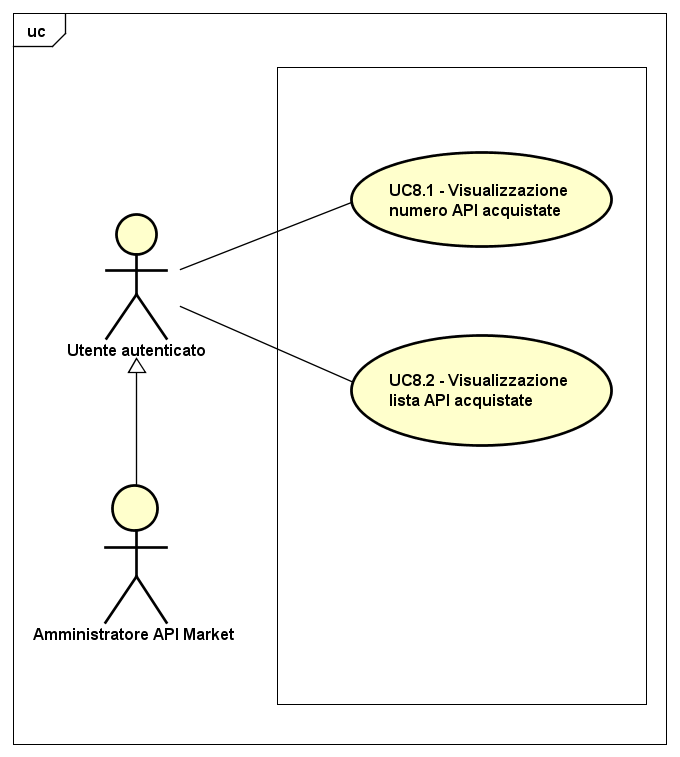
\includegraphics[scale=0.45]{UML/UC8.png}
	\caption{UC8: Visualizzazione API acquistate}
\end{figure}

\begin{longtable}{ l | p{11cm}}
	\hline
	\rowcolor{Gray}
	\multicolumn{2}{c}{UC8 - Visualizzazione API acquistate}\\
	\hline
	 \textbf{Attori} & Utente autenticato, Amministratore API Market \\
	\textbf{Descrizione} & L'attore visualizza le API da lui acquistate \\
	\textbf{Pre-Condizioni} & L'attore si trova nella schermata relativa alle API da lui acquistate \\
	\textbf{Post-Condizioni} & L'attore ha visualizzato le API da lui acquistate \\
	\textbf{Scenario Principale} & 
	\begin{enumerate*}[label=(\arabic*.),itemjoin={\newline}]
		\item L'attore può visualizzare il numero delle API acquistate e attive (UC8.1)
		\item L'attore può visualizzare la lista delle API acquistate e attive (UC8.2)
	\end{enumerate*}\\
\end{longtable}

\subsubsection{Caso d'uso UC8.1: Visualizzazione numero API acquistate}
\label{UC8_1}

\begin{minipage}{\linewidth}
	\begin{tabular}{ l | p{11cm}}
		\hline
		\rowcolor{Gray}
		\multicolumn{2}{c}{UC8.1 - Visualizzazione numero API acquistate} \\
		\hline
		\textbf{Attori} & Utente autenticato, Amministratore API Market \\
		\textbf{Descrizione} & L'attore visualizza il numero di API da lui acquistate \\
		\textbf{Pre-Condizioni} & L'attore si trova nella schermata relativa alle API da lui acquistate \\
		\textbf{Post-Condizioni} & L'attore ha visualizzato il numero delle API da lui acquistate \\
		\textbf{Scenario Principale} & 
		\begin{enumerate*}[label=(\arabic*.),itemjoin={\newline}]
			\item L'attore può visualizzare il numero di API acquistate
		\end{enumerate*}\\
	\end{tabular}
\end{minipage}

\newpage
\subsubsection{Caso d'uso UC8.2: Visualizzazione lista API acquistate}
\label{UC8_2}
\begin{figure}[ht]
	\centering
	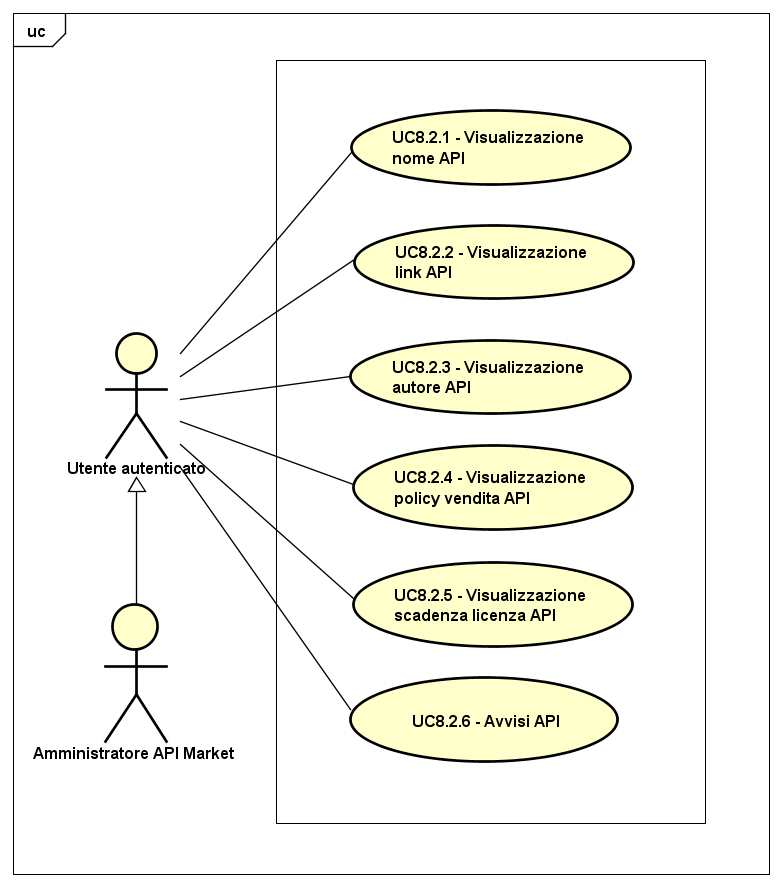
\includegraphics[scale=0.45]{UML/UC8_2.png}
	\caption{UC8.2: Visualizzazione lista API acquistate}
\end{figure}

\begin{minipage}{\linewidth}
	\begin{tabular}{ l | p{11cm}}
		\hline
		\rowcolor{Gray}
		\multicolumn{2}{c}{UC8.2 - Visualizzazione lista API acquistate} \\
		\hline
		\textbf{Attori} & Utente autenticato, Amministratore API Market \\
		\textbf{Descrizione} & L'attore visualizza la lista delle API da lui acquistate \\
		\textbf{Pre-Condizioni} & L'attore si trova nella schermata relativa alle API da lui acquistate \\
		\textbf{Post-Condizioni} & L'attore ha visualizzato la lista delle API da lui acquistate \\
		\textbf{Scenario Principale} & 
		\begin{enumerate*}[label=(\arabic*.),itemjoin={\newline}]
			\item L'attore può visualizzare il nome dell'API (UC8.2.1)
			\item L'attore può visualizzare il link alla pagina di visualizzazione API (UC8.2.2)
			\item L'attore può visualizzare il nome dell'autore dell'API (UC8.2.3)
			\item L'attore può visualizzare la policy divendita dell'API (UC8.2.4)
			\item L'attore può visualizzare il parametro di scadenza, in base al contratto,  della propria licenza per l'API (UC8.2.5)
			\item L'attore può visualizzare gli avvisi riguardo l'API (UC8.2.6)
		\end{enumerate*}\\
	\end{tabular}
\end{minipage}

\paragraph{Caso d'uso UC8.2.1: Visualizzazione nome API}
\label{UC8_2_1}

\begin{minipage}{\linewidth}
	\begin{tabular}{ l | p{11cm}}
		\hline
		\rowcolor{Gray}
		\multicolumn{2}{c}{UC8.2.1 - Visualizzazione nome API} \\
		\hline
		\textbf{Attori} & Utente autenticato, Amministratore API Market \\
		\textbf{Descrizione} & L'attore visualizza nella lista il nome dell'API \\
		\textbf{Pre-Condizioni} & L'attore si trova nella schermata relativa alle API da lui acquistate \\
		\textbf{Post-Condizioni} & L'attore ha visualizzato nella lista il nome dell'API \\
		\textbf{Scenario Principale} & 
		\begin{enumerate*}[label=(\arabic*.),itemjoin={\newline}]
			\item L'attore può visualizzare nella lista il nome dell'API
		\end{enumerate*}\\
	\end{tabular}
\end{minipage}

\paragraph{Caso d'uso UC8.2.2: Visualizzazione link API}
\label{UC8_2_2}

\begin{minipage}{\linewidth}
	\begin{tabular}{ l | p{11cm}}
		\hline
		\rowcolor{Gray}
		\multicolumn{2}{c}{UC8.2.2 - Visualizzazione link API} \\
		\hline
		\textbf{Attori} & Utente autenticato, Amministratore API Market \\
		\textbf{Descrizione} & L'attore visualizza nella lista il link alla visualizzazione dell'API \\
		\textbf{Pre-Condizioni} & L'attore si trova nella schermata di visualizzazione delle API acquistate \\
		\textbf{Post-Condizioni} & L'attore ha visualizzato nella lista il link alla visualizzazione dell'API \\
		\textbf{Scenario Principale} & 
		\begin{enumerate*}[label=(\arabic*.),itemjoin={\newline}]
			\item L'attore può visualizzare nella lista il link alla visualizzazione dell'API, che lo reindirizzerà ad UC7 per l'API in questione
		\end{enumerate*}\\
	\end{tabular}
\end{minipage}

\paragraph{Caso d'uso UC8.2.3: Visualizzazione nome autore API}
\label{UC8_2_3}

\begin{minipage}{\linewidth}
	\begin{tabular}{ l | p{11cm}}
		\hline
		\rowcolor{Gray}
		\multicolumn{2}{c}{UC8.2.3 - Visualizzazione nome autore API} \\
		\hline
		\textbf{Attori} & Utente autenticato, Amministratore API Market \\
		\textbf{Descrizione} & L'attore visualizza nella lista il nome dell'autore dell'API \\
		\textbf{Pre-Condizioni} & L'attore si trova nella schermata relativa alle API da lui acquistate \\
		\textbf{Post-Condizioni} & L'attore ha visualizzato nella lista il nome dell'autore dell'API \\
		\textbf{Scenario Principale} & 
		\begin{enumerate*}[label=(\arabic*.),itemjoin={\newline}]
			\item L'attore può visualizzare nella lista il nome dell'autore dell'API
		\end{enumerate*}\\
	\end{tabular}
\end{minipage}

\paragraph{Caso d'uso UC8.2.4: Visualizzazione policy vendita API}
\label{UC8_2_4}

\begin{minipage}{\linewidth}
	\begin{tabular}{ l | p{11cm}}
		\hline
		\rowcolor{Gray}
		\multicolumn{2}{c}{UC8.2.4 - Visualizzazione policy vendita API} \\
		\hline
		\textbf{Attori} & Utente autenticato, Amministratore API Market \\
		\textbf{Descrizione} & L'attore visualizza nella lista la policy di vendita dell'API \\
		\textbf{Pre-Condizioni} & L'attore si trova nella schermata relativa alle API da lui acquistate \\
		\textbf{Post-Condizioni} & L'attore ha visualizzato nella lista la policy di vendita dell'API \\
		\textbf{Scenario Principale} & 
		\begin{enumerate*}[label=(\arabic*.),itemjoin={\newline}]
			\item L'attore può visualizzare nella lista la policy di vendita dell'API
		\end{enumerate*}\\
	\end{tabular}
\end{minipage}

\paragraph{Caso d'uso UC8.2.5: Visualizzazione scadenza licenza}
\label{UC8_2_5}

\begin{minipage}{\linewidth}
	\begin{tabular}{ l | p{11cm}}
		\hline
		\rowcolor{Gray}
		\multicolumn{2}{c}{UC8.2.3 - Visualizzazione scadenza licenza} \\
		\hline
		\textbf{Attori} & Utente autenticato, Amministratore API Market \\
		\textbf{Descrizione} & L'attore visualizza nella lista la data di scadenza della propria licenza per l'API \\
		\textbf{Pre-Condizioni} & L'attore si trova nella schermata relativa alle API da lui acquistate \\
		\textbf{Post-Condizioni} & L'attore ha visualizzato nella lista il parametro di scadenza dell'API \\
		\textbf{Scenario Principale} & 
		\begin{enumerate*}[label=(\arabic*.),itemjoin={\newline}]
			\item L'attore può visualizzare nella lista il parametro di scadenza della propria licenza per l'API
		\end{enumerate*}\\
	\end{tabular}
\end{minipage}

\paragraph{Caso d'uso UC8.2.6: Avvisi API}
\label{UC8_2_6}

\begin{minipage}{\linewidth}
	\begin{tabular}{ l | p{11cm}}
		\hline
		\rowcolor{Gray}
		\multicolumn{2}{c}{UC8.2.6 - Avvisi API} \\
		\hline
		\textbf{Attori} & Utente autenticato, Amministratore API Market \\
		\textbf{Descrizione} & L'attore visualizza nella lista gli avvisi riguardanti l'API \\
		\textbf{Pre-Condizioni} & L'attore si trova nella schermata relativa alle API da lui acquistate \\
		\textbf{Post-Condizioni} & L'attore ha visualizzato nella lista gli avvisi riguardanti l'API \\
		\textbf{Scenario Principale} & 
		\begin{enumerate*}[label=(\arabic*.),itemjoin={\newline}]
			\item L'attore può visualizzare nella lista gli avvisi riguardanti l'API (E.g: cancellazione, manutenzione)
		\end{enumerate*}\\
	\end{tabular}
\end{minipage}
\newpage
\subsection{Caso d'uso UC9: Acquisto API}
\label{UC9}
\begin{figure}[ht]
	\centering
	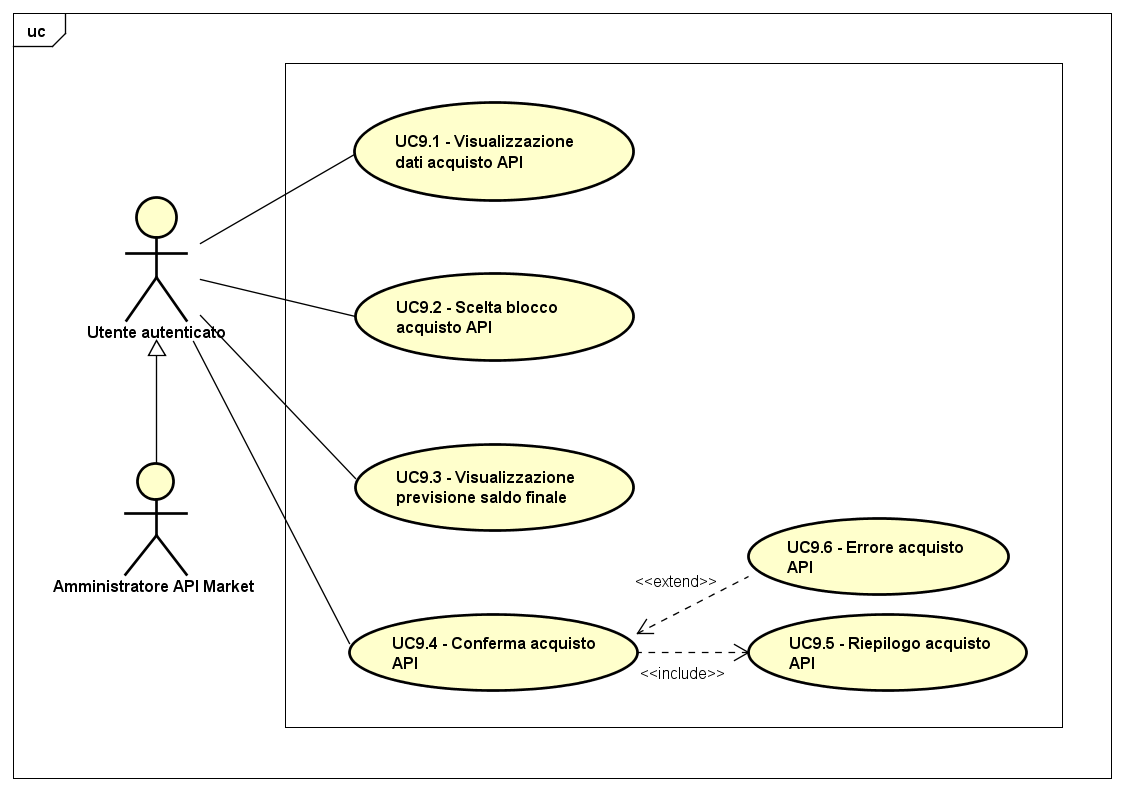
\includegraphics[scale=0.45]{UML/UC9.png}
	\caption{UC9: Acquisto API}
\end{figure}

\begin{longtable}{ l | p{11cm}}
	\hline
	\rowcolor{Gray}
	\multicolumn{2}{c}{UC9 - Acquisto API}\\
	\hline
	\textbf{Attori} & Utente autenticato, Amministratore API Market \\
	\textbf{Descrizione} & L'attore effettua l'acquisto dell'API selezionata tramite i crediti da lui posseduti \\
	\textbf{Pre-Condizioni} & L'attore ha selezionato una API e si trova nella relativa schermata di acquisto \\
	\textbf{Post-Condizioni} & L'attore ha acquistato l'API selezionata \\
	\textbf{Scenario Principale} & 
	\begin{enumerate*}[label=(\arabic*.),itemjoin={\newline}]
		\item L'attore può visualizzare i dati d'acquisto dell'API (UC9.1)
		\item L'attore può scegliere la licenza API desiderata (UC9.2)
		\item L'attore può visualizzare il saldo preventivato in seguito all'acquisto dell'API con la licenza selezionata (UC9.3)
		\item L'attore può confermare l'acquisto (UC9.4), venendo reindirizzato ad una schermata di riepilogo (UC9.5)
	\end{enumerate*}\\
	\textbf{Scenari Alternativi} & 
	\begin{enumerate*}[label=(\arabic*.),itemjoin={\newline}]
		\item L'attore può visualizzare un messaggio di errore (E.g: saldo non sufficiente) e la transazione non avviene (UC9.6)
		\item L'attore può scegliere la licenza API per numero di chiamate (UC9.2.1)
		\item L'attore può scegliere la licenza API per tempo di utilizzo (UC9.2.2)
		\item L'attore può scegliere la licenza API per traffico (UC9.2.3)
	\end{enumerate*}\\
\end{longtable}

\subsubsection{Caso d'uso UC9.1: Visualizzazione dati acquisto API}
\label{UC9_1}

\begin{minipage}{\linewidth}
	\begin{tabular}{ l | p{11cm}}
		\hline
		\rowcolor{Gray}
		\multicolumn{2}{c}{UC9.1 - Visualizzazione dati acquisto API} \\
		\hline
		\textbf{Attori} & Utente autenticato, Amministratore API Market \\
		\textbf{Descrizione} & L'attore visualizza i dati d'acquisto dell'API \\
		\textbf{Pre-Condizioni} & L'attore si trova nella schermata di acquisto dell'API \\
		\textbf{Post-Condizioni} & L'attore ha visualizzato i dati d'acquisto dell'API \\
		\textbf{Scenario Principale} & 
		\begin{enumerate*}[label=(\arabic*.),itemjoin={\newline}]
			\item L'attore può visualizzare il nome dell'API (UC9.1.1)
			\item L'attore può visualizzare l'autore dell'API (UC9.1.2)
		\end{enumerate*}\\
	\end{tabular}
\end{minipage}

\paragraph{Caso d'uso UC9.1.1: Visualizzazione nome API}
\label{UC9_1_1}

\begin{minipage}{\linewidth}
	\begin{tabular}{ l | p{11cm}}
		\hline
		\rowcolor{Gray}
		\multicolumn{2}{c}{UC9.1.1 - Visualizzazione nome API} \\
		\hline
		\textbf{Attori} & Utente autenticato, Amministratore API Market \\
		\textbf{Descrizione} & L'attore visualizza il nome dell'API \\
		\textbf{Pre-Condizioni} & L'attore si trova nella schermata di acquisto dell'API \\
		\textbf{Post-Condizioni} & L'attore ha visualizzato il nome dell'API \\
		\textbf{Scenario Principale} & 
		\begin{enumerate*}[label=(\arabic*.),itemjoin={\newline}]
			\item L'attore può visualizzare il nome dell'API
		\end{enumerate*}\\
	\end{tabular}
\end{minipage}

\paragraph{Caso d'uso UC9.1.2: Visualizzazione autore API}
\label{UC9_1_2}

\begin{minipage}{\linewidth}
	\begin{tabular}{ l | p{11cm}}
		\hline
		\rowcolor{Gray}
		\multicolumn{2}{c}{UC9.1.2 - Visualizzazione autore API} \\
		\hline
		\textbf{Attori} & Utente autenticato, Amministratore API Market \\
		\textbf{Descrizione} & L'attore visualizza l'autore dell'API \\
		\textbf{Pre-Condizioni} & L'attore si trova nella schermata di acquisto dell'API \\
		\textbf{Post-Condizioni} & L'attore ha visualizzato l'autore dell'API \\
		\textbf{Scenario Principale} & 
		\begin{enumerate*}[label=(\arabic*.),itemjoin={\newline}]
			\item L'attore può visualizzare l'autore dell'API
		\end{enumerate*}\\
	\end{tabular}
\end{minipage}

\paragraph{Caso d'uso UC9.1.3: Visualizzazione policy vendita API}
\label{UC9_1_3}

\begin{minipage}{\linewidth}
	\begin{tabular}{ l | p{11cm}}
		\hline
		\rowcolor{Gray}
		\multicolumn{2}{c}{UC9.1.3 - Visualizzazione policy vendita API} \\
		\hline
		\textbf{Attori} & Utente autenticato, Amministratore API Market \\
		\textbf{Descrizione} & L'attore visualizza la policy di vendita dell'API \\
		\textbf{Pre-Condizioni} & L'attore si trova nella schermata di acquisto dell'API \\
		\textbf{Post-Condizioni} & L'attore ha visualizzato la policy di vendita dell'API \\
		\textbf{Scenario Principale} & 
		\begin{enumerate*}[label=(\arabic*.),itemjoin={\newline}]
			\item L'attore può visualizzare la policy di vendita dell'API
		\end{enumerate*}\\
	\end{tabular}
\end{minipage}

\subsubsection{Caso d'uso UC9.2: Scelta blocco acquisto API}
\label{UC9_2}

\begin{minipage}{\linewidth}
	\begin{tabular}{ l | p{11cm}}
		\hline
		\rowcolor{Gray}
		\multicolumn{2}{c}{UC9.2 - Scelta blocco acquisto API} \\
		\hline
		\textbf{Attori} & Utente autenticato, Amministratore API Market \\
		\textbf{Descrizione} & L'attore sceglie il blocco da acquistare in base alla policy di vendita dell'API \\
		\textbf{Pre-Condizioni} & L'attore ha selezionato una API e si trova nella relativa schermata di acquisto \\
		\textbf{Post-Condizioni} & L'attore ha scelto il blocco da acquistare in base alla policy di vendita dell'API \\
		\textbf{Scenario Principale} & 
		\begin{enumerate*}[label=(\arabic*.),itemjoin={\newline}]
			\item L'attore può scegliere il blocco da acquistare in base alla policy di vendita dell'API
		\end{enumerate*}\\
	\end{tabular}
\end{minipage}

\subsubsection{Caso d'uso UC9.3: Visualizzazione previsione saldo finale}
\label{UC9_3}

\begin{minipage}{\linewidth}
	\begin{tabular}{ l | p{11cm}}
		\hline
		\rowcolor{Gray}
		\multicolumn{2}{c}{UC9.3 - Visualizzazione previsione saldo finale} \\
		\hline
		\textbf{Attori} & Utente autenticato, Amministratore API Market \\
		\textbf{Descrizione} & L'attore visualizza una previsione del proprio saldo crediti in seguito all'acquisto \\
		\textbf{Pre-Condizioni} & L'attore ha selezionato una API e si trova nella relativa schermata di acquisto \\
		\textbf{Post-Condizioni} & L'attore ha visualizzato una previsione del proprio saldo in seguito all'acquisto \\
		\textbf{Scenario Principale} & 
		\begin{enumerate*}[label=(\arabic*.),itemjoin={\newline}]
			\item L'attore può visualizzare una previsione del proprio saldo finale qualora acquistasse l'API con il blocco di acquisto scelto in UC9.2
		\end{enumerate*}\\
	\end{tabular}
\end{minipage}

\subsubsection{Caso d'uso UC9.4: Conferma acquisto API}
\label{UC9_4}

\begin{minipage}{\linewidth}
	\begin{tabular}{ l | p{11cm}}
		\hline
		\rowcolor{Gray}
		\multicolumn{2}{c}{UC9.4 - Conferma acquisto API} \\
		\hline
		\textbf{Attori} & Utente autenticato, Amministratore API Market \\
		\textbf{Descrizione} & L'attore può confermare l'acquisto dell'API, portando a termine la transazione, ricevendo un'email di riepilogo e visualizzando una schermata di riepilogo dell'acquisto appena realizzato \\
		\textbf{Pre-Condizioni} & L'attore ha selezionato una API e si trova nella relativa schermata di acquisto \\
		\textbf{Post-Condizioni} & L'attore ha confermato l'acquisto dell'API \\
		\textbf{Scenario Principale} & 
		\begin{enumerate*}[label=(\arabic*.),itemjoin={\newline}]
			\item L'attore può confermare l'acquisto dell'API, portando a termine la transazione, ricevendo un'email di riepilogo e visualizzando una schermata di riepilogo dell'acquisto appena realizzato (UC9.5)
		\end{enumerate*}\\
	\end{tabular}
\end{minipage}

\newpage
\subsubsection{Caso d'uso UC9.5: Riepilogo acquisto API}
\label{UC9_5}
\begin{figure}[ht]
	\centering
	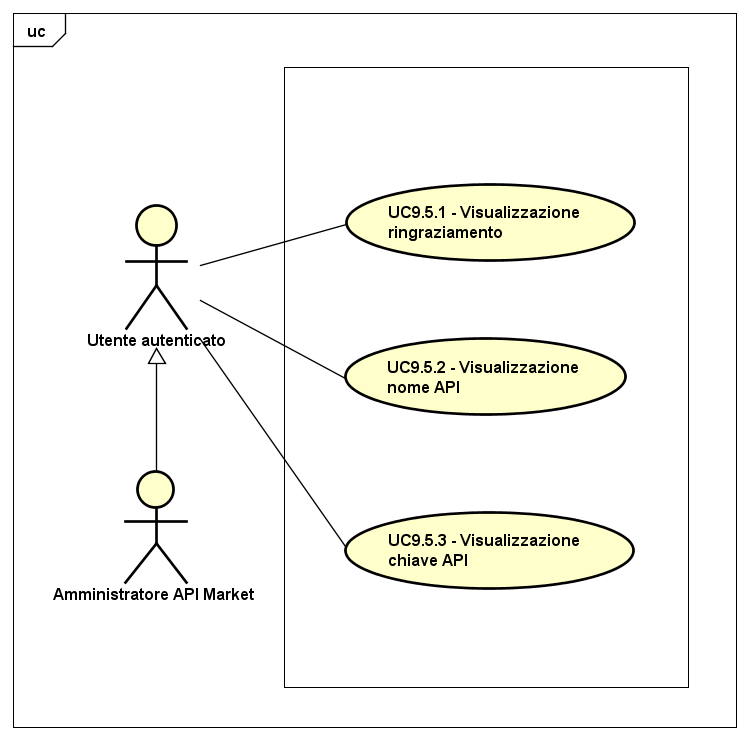
\includegraphics[scale=0.45]{UML/UC9_5.png}
	\caption{UC9.5: Riepilogo acquisto API}
\end{figure}

\begin{minipage}{\linewidth}
	\begin{tabular}{ l | p{11cm}}
		\hline
		\rowcolor{Gray}
		\multicolumn{2}{c}{UC9.5 - Riepilogo acquisto API} \\
		\hline
		\textbf{Attori} & Utente autenticato, Amministratore API Market \\
		\textbf{Descrizione} & L'attore conferma l'acquisto dell'API, portando a termine la transazione e visualizzando un messaggio di ringraziamento \\
		\textbf{Pre-Condizioni} & L'attore ha confermato l'acquisto per l'API \\
		\textbf{Post-Condizioni} & L'attore ha visualizzato il riepilogo dell'acquisto appena realizzato \\
		\textbf{Scenario Principale} & 
		\begin{enumerate*}[label=(\arabic*.),itemjoin={\newline}]
			\item L'attore può visualizzare un messaggio di ringraziamento (UC9.5.1)
			\item L'attore può visualizzare il nome dell'API appena acquistata (UC9.5.2)
			\item L'attore può visualizzare la chiave dell'API appena acquistata (UC9.5.3)
		\end{enumerate*}\\
	\end{tabular}
\end{minipage}

\paragraph{Caso d'uso UC9.5.1: Visualizzazione ringraziamento}
\label{UC9_5_1}

\begin{minipage}{\linewidth}
	\begin{tabular}{ l | p{11cm}}
		\hline
		\rowcolor{Gray}
		\multicolumn{2}{c}{UC9.5.1 - Visualizzazione ringraziamento} \\
		\hline
		\textbf{Attori} & Utente autenticato, Amministratore API Market \\
		\textbf{Descrizione} & L'attore visualizza un messaggio di ringraziamento \\
		\textbf{Pre-Condizioni} & L'attore si trova nella schermata di riepilogo acquisto dell'API \\
		\textbf{Post-Condizioni} & L'attore ha visualizzato un messaggio di ringraziamento \\
		\textbf{Scenario Principale} & 
		\begin{enumerate*}[label=(\arabic*.),itemjoin={\newline}]
			\item L'attore può visualizzare un messaggio di ringraziamento
		\end{enumerate*}\\
	\end{tabular}
\end{minipage}

\paragraph{Caso d'uso UC9.5.2: Visualizzazione nome API acquistata}
\label{UC9_5_2}

\begin{minipage}{\linewidth}
	\begin{tabular}{ l | p{11cm}}
		\hline
		\rowcolor{Gray}
		\multicolumn{2}{c}{UC9.5.2 - Visualizzazione nome API acquistata} \\
		\hline
		\textbf{Attori} & Utente autenticato, Amministratore API Market \\
		\textbf{Descrizione} & L'attore visualizza il nome dell'API acquistata \\
		\textbf{Pre-Condizioni} & L'attore si trova nella schermata di riepilogo acquisto dell'API \\
		\textbf{Post-Condizioni} & L'attore ha visualizzato il nome dell'API acquistata \\
		\textbf{Scenario Principale} & 
		\begin{enumerate*}[label=(\arabic*.),itemjoin={\newline}]
			\item L'attore può visualizzare il nome dell'API acquistata
		\end{enumerate*}\\
	\end{tabular}
\end{minipage}

\paragraph{Caso d'uso UC9.5.3: Visualizzazione chiave API acquistata}
\label{UC9_5_3}

\begin{minipage}{\linewidth}
	\begin{tabular}{ l | p{11cm}}
		\hline
		\rowcolor{Gray}
		\multicolumn{2}{c}{UC9.5.3 - Visualizzazione chiave API acquistata} \\
		\hline
		\textbf{Attori} & Utente autenticato, Amministratore API Market \\
		\textbf{Descrizione} & L'attore visualizza la chiave dell'API acquistata \\
		\textbf{Pre-Condizioni} & L'attore si trova nella schermata di riepilogo acquisto dell'API \\
		\textbf{Post-Condizioni} & L'attore ha visualizzato la chiave dell'API acquistata \\
		\textbf{Scenario Principale} & 
		\begin{enumerate*}[label=(\arabic*.),itemjoin={\newline}]
			\item L'attore può visualizzare la chiave dell'API acquistata
		\end{enumerate*}\\
	\end{tabular}
\end{minipage}

\subsubsection{Caso d'uso UC9.6: Errore acquisto API}
\label{UC9_6}

\begin{minipage}{\linewidth}
	\begin{tabular}{ l | p{11cm}}
		\hline
		\rowcolor{Gray}
		\multicolumn{2}{c}{UC9.6 - Errore acquisto API} \\
		\hline
		\textbf{Attori} & Utente autenticato, Amministratore API Market \\
		\textbf{Descrizione} & L'attore visualizza un messaggio di errore e la transazione non avviene \\
		\textbf{Pre-Condizioni} & L'attore ha confermato l'acquisto per una API ma si è verificato un errore \\
		\textbf{Post-Condizioni} & L'attore ha visualizzato un errore relativo all'acquisto, con opportuna descrizione \\
		\textbf{Scenario Principale} & 
		\begin{enumerate*}[label=(\arabic*.),itemjoin={\newline}]
			\item L'attore può visualizzare un messaggio di errore e la transazione non avviene (E.g: L'API è sospesa)
		\end{enumerate*}\\
	\end{tabular}
\end{minipage}
\newpage
\subsection{Caso d'uso UC10: Visualizzazione API registrate}
\label{UC10}
\begin{figure}[ht]
	\centering
	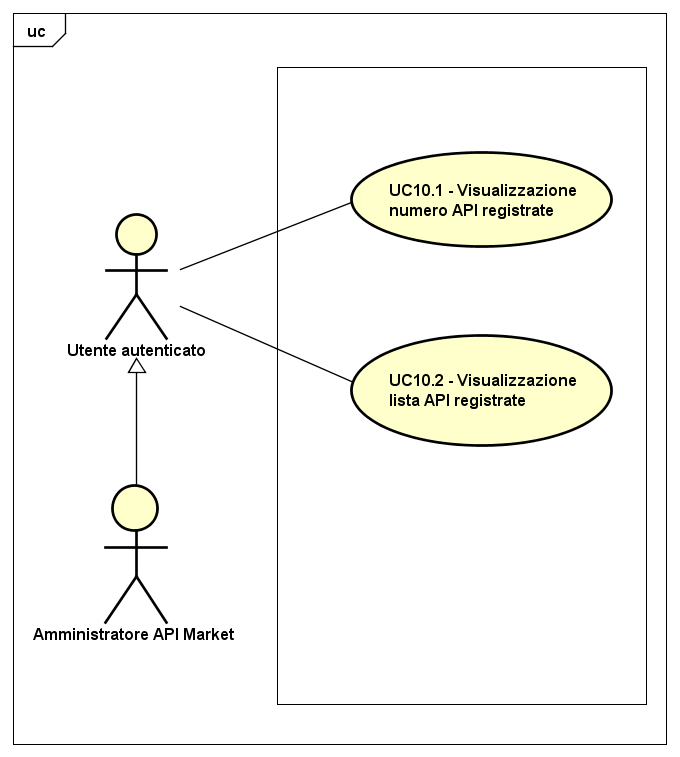
\includegraphics[scale=0.45]{UML/UC10.png}
	\caption{UC10: Visualizzazione API registrate}
\end{figure}

\begin{longtable}{ l | p{11cm}}
	\hline
	\rowcolor{Gray}
	\multicolumn{2}{c}{UC10 - Visualizzazione API registrate}\\
	\hline
	\textbf{Attori} & Utente autenticato, Amministratore API Market \\
	\textbf{Descrizione} & L'attore visualizza le API da lui registrate \\
	\textbf{Pre-Condizioni} & L'attore si trova nella schermata relativa alle API da lui registrate \\
	\textbf{Post-Condizioni} & L'attore ha visualizzato le API da lui registrate \\
	\textbf{Scenario Principale} & 
	\begin{enumerate*}[label=(\arabic*.),itemjoin={\newline}]
		\item L'attore può visualizzare il numero delle API da lui registrate (UC10.1)
		\item L'attore può visualizzare la lista delle API da lui registrate (UC10.2)
	\end{enumerate*}\\
\end{longtable}

\subsubsection{Caso d'uso UC10.1: Visualizzazione numero API registrate}
\label{UC10_1}

\begin{minipage}{\linewidth}
	\begin{tabular}{ l | p{11cm}}
		\hline
		\rowcolor{Gray}
		\multicolumn{2}{c}{UC10.1 - Visualizzazione numero API registrate} \\
		\hline
		\textbf{Attori} & Utente autenticato, Amministratore API Market \\
		\textbf{Descrizione} & L'attore visualizza il numero di API da lui registrate \\
		\textbf{Pre-Condizioni} & L'attore si trova nella schermata relativa alle API da lui registrate \\
		\textbf{Post-Condizioni} & L'attore ha visualizzato il numero delle API da lui registrate \\
		\textbf{Scenario Principale} & 
		\begin{enumerate*}[label=(\arabic*.),itemjoin={\newline}]
			\item L'attore può visualizzare il numero di API da lui registrate
		\end{enumerate*}\\
	\end{tabular}
\end{minipage}

\newpage
\subsubsection{Caso d'uso UC10.2: Visualizzazione lista API registrate}
\label{UC10_2}
\begin{figure}[ht]
	\centering
	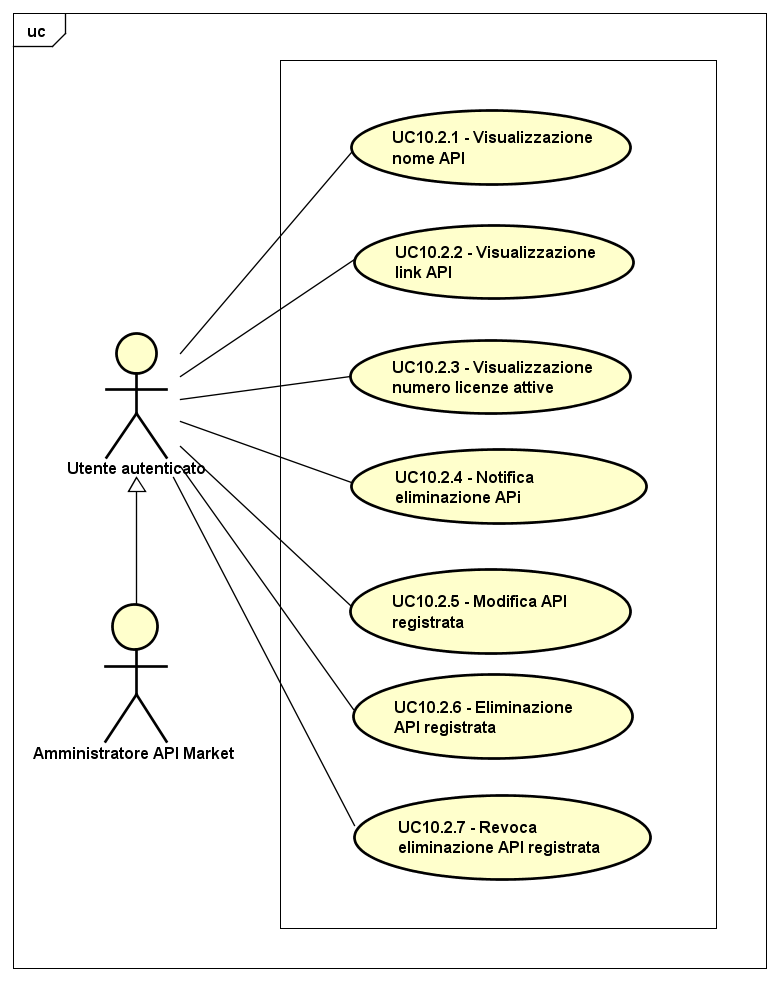
\includegraphics[scale=0.45]{UML/UC10_2.png}
	\caption{UC10.2: Visualizzazione lista API registrate}
\end{figure}

\begin{minipage}{\linewidth}
	\begin{tabular}{ l | p{11cm}}
		\hline
		\rowcolor{Gray}
		\multicolumn{2}{c}{UC10.2 - Visualizzazione lista API registrate} \\
		\hline
		\textbf{Attori} & Utente autenticato, Amministratore API Market \\
		\textbf{Descrizione} & L'attore visualizza la lista di ogni API da lui registrata \\
		\textbf{Pre-Condizioni} & L'attore si trova nella schermata relativa alle API da lui registrate \\
		\textbf{Post-Condizioni} & L'attore ha visualizzato la lista delle API da lui registrate \\
		\textbf{Scenario Principale} & 
		\begin{enumerate*}[label=(\arabic*.),itemjoin={\newline}]
			\item L'attore può visualizzare il nome di ogni API da lui registrata (UC10.2.1)
			\item L'attore può visualizzare il link alla pagina di visualizzazione API di ogni API da lui registrata (UC10.2.2)
			\item L'attore può visualizzare il numero di licenze attive di ogni API da lui registrata (UC10.2.3)
			\item L'attore può modificare ogni API da lui registrata (UC10.2.4)
			\item L'attore può eliminare ogni API da lui registrata (UC10.2.5)
		\end{enumerate*}\\
	\end{tabular}
\end{minipage}

\paragraph{Caso d'uso UC10.2.1: Visualizzazione nome API}
\label{UC10_2_1}

\begin{minipage}{\linewidth}
	\begin{tabular}{ l | p{11cm}}
		\hline
		\rowcolor{Gray}
		\multicolumn{2}{c}{UC10.2.1 - Visualizzazione nome API} \\
		\hline
		\textbf{Attori} & Utente autenticato, Amministratore API Market \\
		\textbf{Descrizione} & L'attore visualizza nella lista il nome di ogni API da lui registrata \\
		\textbf{Pre-Condizioni} & L'attore si trova nella schermata relativa alle API da lui registrate \\
		\textbf{Post-Condizioni} & L'attore ha visualizzato nella lista il nome di ogni API da lui registrata \\
		\textbf{Scenario Principale} & 
		\begin{enumerate*}[label=(\arabic*.),itemjoin={\newline}]
			\item L'attore può visualizzare nella lista il nome di ogni API da lui registrata
		\end{enumerate*}\\
	\end{tabular}
\end{minipage}

\paragraph{Caso d'uso UC10.2.2: Visualizzazione link API}
\label{UC10_2_2}

\begin{minipage}{\linewidth}
	\begin{tabular}{ l | p{11cm}}
		\hline
		\rowcolor{Gray}
		\multicolumn{2}{c}{UC10.2.2 - Visualizzazione link API} \\
		\hline
		\textbf{Attori} & Utente autenticato, Amministratore API Market \\
		\textbf{Descrizione} & L'attore visualizza nella lista il link alla visualizzazione dell'API  \\
		\textbf{Pre-Condizioni} & L'attore si trova nella schermata relativa alle API da lui registrate \\
		\textbf{Post-Condizioni} & L'attore ha visualizzato nella lista il link alla visualizzazione dell'API \\
		\textbf{Scenario Principale} & 
		\begin{enumerate*}[label=(\arabic*.),itemjoin={\newline}]
			\item L'attore può visualizzare nella lista il link alla visualizzazione dell'API, che lo reindirizzerà ad UC7 per l'API in questione
		\end{enumerate*}\\
	\end{tabular}
\end{minipage}

\paragraph{Caso d'uso UC10.2.3: Visualizzazione numero licenze attive}
\label{UC10_2_3}

\begin{minipage}{\linewidth}
	\begin{tabular}{ l | p{11cm}}
		\hline
		\rowcolor{Gray}
		\multicolumn{2}{c}{UC10.2.3 - Visualizzazione numero licenze attive} \\
		\hline
		\textbf{Attori} & Utente autenticato, Amministratore API Market \\
		\textbf{Descrizione} & L'attore visualizza nella lista il numero di licenze attive per ogni API da lui registrata \\
		\textbf{Pre-Condizioni} & L'attore si trova nella schermata relativa alle API da lui registrate \\
		\textbf{Post-Condizioni} & L'attore ha visualizzato nella lista il numero di licenze attive per ogni API da lui registrata \\
		\textbf{Scenario Principale} & 
		\begin{enumerate*}[label=(\arabic*.),itemjoin={\newline}]
			\item L'attore può visualizzare nella lista il numero di licenze attive per ogni API da lui registrata
		\end{enumerate*}\\
	\end{tabular}
\end{minipage}

\paragraph{Caso d'uso UC10.2.4: Notifica eliminazione API}
\label{UC10_2_1}

\begin{minipage}{\linewidth}
	\begin{tabular}{ l | p{11cm}}
		\hline
		\rowcolor{Gray}
		\multicolumn{2}{c}{UC10.2.1 - Notifica eliminazione API} \\
		\hline
		\textbf{Attori} & Utente autenticato, Amministratore API Market \\
		\textbf{Descrizione} & Per ogni API da lui registrata nella lista, l'attore visualizza se questa sia in fase di eliminazione \\
		\textbf{Pre-Condizioni} & L'attore si trova nella schermata relativa alle API da lui registrate \\
		\textbf{Post-Condizioni} & Per ogni API da lui registrata nella lista, l'attore ha visualizzato se questa sia in fase di eliminazione \\
		\textbf{Scenario Principale} & 
		\begin{enumerate*}[label=(\arabic*.),itemjoin={\newline}]
			\item Per ogni API da lui registrata nella lista, l'attore può visualizzare se questa sia in fase di eliminazione
		\end{enumerate*}\\
	\end{tabular}
\end{minipage}

\newpage
\paragraph{Caso d'uso UC10.2.5: Modifica API registrata}
\label{UC10_2_5}
\begin{figure}[ht]
	\centering
	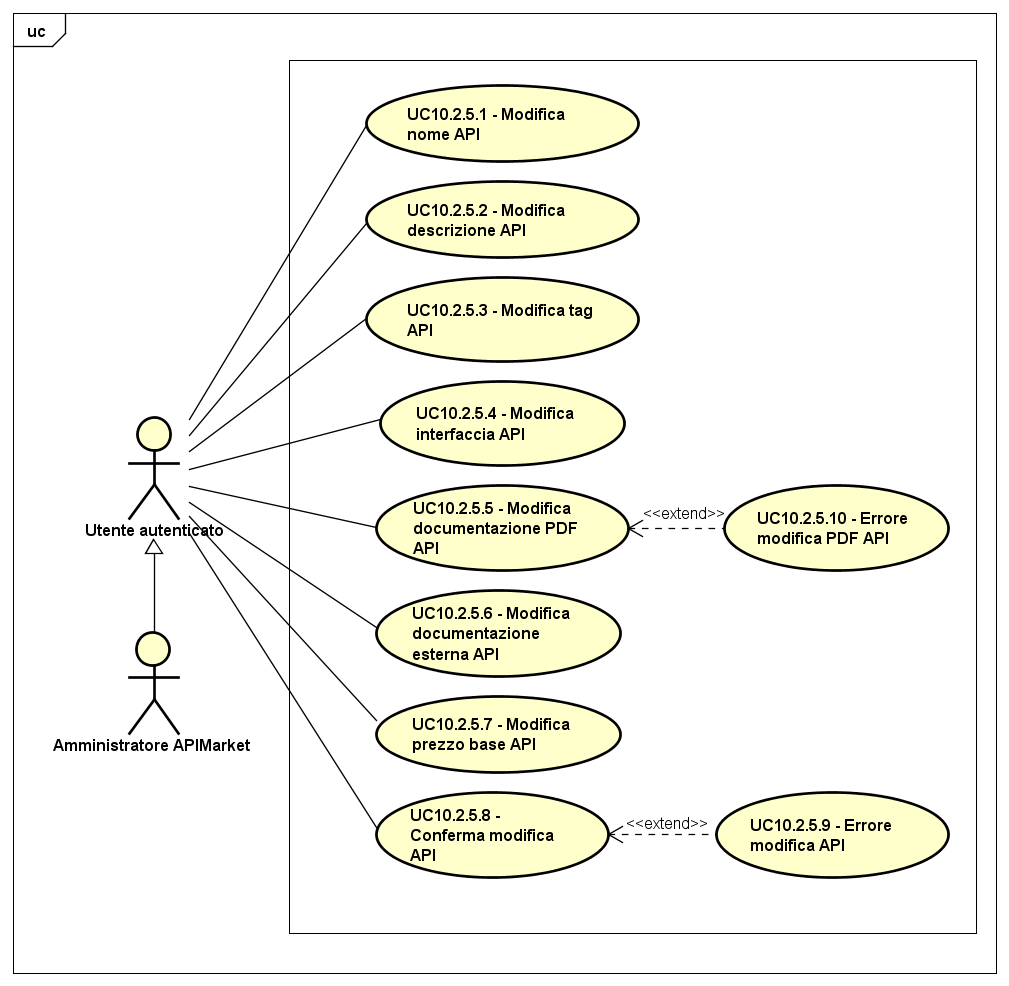
\includegraphics[scale=0.45]{UML/UC10_2_5.png}
	\caption{UC10.2.5: Modifica API registrata}
\end{figure}

\begin{minipage}{\linewidth}
	\begin{tabular}{ l | p{11cm}}
		\hline
		\rowcolor{Gray}
		\multicolumn{2}{c}{UC10.2.5 - Modifica API registrata} \\
		\hline
		\textbf{Attori} & Utente autenticato, Amministratore API Market \\
		\textbf{Descrizione} & L'attore modifica una API da lui registrata \\
		\textbf{Pre-Condizioni} & L'attore si trova nella schermata relativa alle API da lui registrate \\
		\textbf{Post-Condizioni} & L'attore ha modificato un API registrata \\
		\textbf{Scenario Principale} & 
		\begin{enumerate*}[label=(\arabic*.),itemjoin={\newline}]
			\item L'attore può modificare il nome dell'API (UC10.2.5.1)
			\item L'attore può modificare la descrizione dell'API (UC10.2.5.2)
			\item L'attore può modificare i tag dell'API (UC10.2.5.3)
			\item L'attore può modificare l'interfaccia dell'API (UC10.2.5.4)
			\item L'attore può modificare il file per la documentazione PDF (UC10.2.5.5)
			\item L'attore può modificare il link per la documentazione esterna (UC10.2.5.6)
			\item L'attore può modificare il prezzo base dell'API (UC10.2.5.7)
			\item L'attore può confermare la modifica dell'API (UC10.2.5.8)
		\end{enumerate*}\\
		\textbf{Scenari Alternativi} & 
		\begin{enumerate*}[label=(\arabic*.),itemjoin={\newline}]
			\item L'attore può visualizzare un messaggio d'errore informativo riguardo la conferma delle modifiche dell'API, e le modifiche non avvengono (UC10.2.5.9)
			\item L'attore può visualizzare un messaggio di errore riguardo al caricamento del file di documentazione PDF dell'API, ed il caricamento del file non avviene (UC10.2.5.10)
		\end{enumerate*}\\
	\end{tabular}
\end{minipage}

\subparagraph{Caso d'uso UC10.2.5.1: Modifica nome API}
\label{UC10_2_5_1}

\begin{minipage}{\linewidth}
	\begin{tabular}{ l | p{11cm}}
		\hline
		\rowcolor{Gray}
		\multicolumn{2}{c}{UC10.2.5.1 - Modifica nome API} \\
		\hline
		\textbf{Attori} & Utente autenticato, Amministratore API Market \\
		\textbf{Descrizione} & L'attore modifica il nome dell'API \\
		\textbf{Pre-Condizioni} & L'attore si trova nella schermata relativa alla modifica di una API registrata, precedentemente selezionata \\
		\textbf{Post-Condizioni} & L'attore ha modificato il nome dell'API selezionata \\
		\textbf{Scenario Principale} & 
		\begin{enumerate*}[label=(\arabic*.),itemjoin={\newline}]
			\item L'attore può modificare il nome dell'API
		\end{enumerate*}\\
	\end{tabular}
\end{minipage}

\subparagraph{Caso d'uso UC10.2.5.2: Modifica descrizione API}
\label{UC10_2_5_2}

\begin{minipage}{\linewidth}
	\begin{tabular}{ l | p{11cm}}
		\hline
		\rowcolor{Gray}
		\multicolumn{2}{c}{UC10.2.5.2 - Modifica descrizione API} \\
		\hline
		\textbf{Attori} & Utente autenticato, Amministratore API Market \\
		\textbf{Descrizione} & L'attore modifica la descrizione dell'API\\
		\textbf{Pre-Condizioni} & L'attore si trova nella schermata relativa alla modifica di una API registrata, precedentemente selezionata \\
		\textbf{Post-Condizioni} & L'attore ha modificato la descrizione dell'API selezionata \\
		\textbf{Scenario Principale} & 
		\begin{enumerate*}[label=(\arabic*.),itemjoin={\newline}]
			\item L'attore può modificare la descrizione dell'API
		\end{enumerate*}\\
	\end{tabular}
\end{minipage}

\subparagraph{Caso d'uso UC10.2.5.3: Modifica tag API}
\label{UC10_2_5_3}

\begin{minipage}{\linewidth}
	\begin{tabular}{ l | p{11cm}}
		\hline
		\rowcolor{Gray}
		\multicolumn{2}{c}{UC10.2.5.3 - Modifica tag API} \\
		\hline
		\textbf{Attori} & Utente autenticato, Amministratore API Market \\
		\textbf{Descrizione} & L'attore modifica i tag dell'API \\
		\textbf{Pre-Condizioni} & L'attore si trova nella schermata relativa alla modifica di una API registrata, precedentemente selezionata \\
		\textbf{Post-Condizioni} & L'attore ha modificato i tag dell'API selezionata \\
		\textbf{Scenario Principale} & 
		\begin{enumerate*}[label=(\arabic*.),itemjoin={\newline}]
			\item L'attore può modificare i tag dell'API
		\end{enumerate*}\\
	\end{tabular}
\end{minipage}

\subparagraph{Caso d'uso UC10.2.5.4: Modifica interfaccia API}
\label{UC10_2_5_4}

\begin{minipage}{\linewidth}
	\begin{tabular}{ l | p{11cm}}
		\hline
		\rowcolor{Gray}
		\multicolumn{2}{c}{UC10.2.5.4 - Modifica interfaccia API} \\
		\hline
		\textbf{Attori} & Utente autenticato, Amministratore API Market \\
		\textbf{Descrizione} & L'attore modifica l'interfaccia dell'API \\
		\textbf{Pre-Condizioni} & L'attore si trova nella schermata relativa alla modifica di una API registrata, precedentemente selezionata \\
		\textbf{Post-Condizioni} & L'attore ha modificato l'interfaccia pubblica dell'API selezionata \\
		\textbf{Scenario Principale} & 
		\begin{enumerate*}[label=(\arabic*.),itemjoin={\newline}]
			\item L'attore può modificare l'interfaccia dell'API
		\end{enumerate*}\\
	\end{tabular}
\end{minipage}

\subparagraph{Caso d'uso UC10.2.5.5: Modifica documentazione PDF API}
\label{UC10_2_5_5}

\begin{minipage}{\linewidth}
	\begin{tabular}{ l | p{11cm}}
		\hline
		\rowcolor{Gray}
		\multicolumn{2}{c}{UC10.2.5.5 - Modifica documentazione PDF API} \\
		\hline
		\textbf{Attori} & Utente autenticato, Amministratore API Market \\
		\textbf{Descrizione} & L'attore carica su API Market un file PDF contenente la nuova documentazione PDF dell'API \\
		\textbf{Pre-Condizioni} & L'attore si trova nella schermata relativa alla modifica di una API registrata, precedentemente selezionata \\
		\textbf{Post-Condizioni} & L'attore ha caricato su API Market un nuovo file PDF contenente la documentazione PDF dell'API \\
		\textbf{Scenario Principale} & 
		\begin{enumerate*}[label=(\arabic*.),itemjoin={\newline}]
			\item L'attore può caricare su API Market un nuovo file PDF contenente la documentazione PDF dell'API
		\end{enumerate*}\\
		\textbf{Scenari Alternativi} & 
		\begin{enumerate*}[label=(\arabic*.),itemjoin={\newline}]
			\item L'attore può visualizzare un messaggio di errore (E.g: formato errato) ed il caricamento del file non avviene (UC10.2.5.10)
		\end{enumerate*}\\
	\end{tabular}
\end{minipage}

\subparagraph{Caso d'uso UC10.2.5.10: Errore modifica PDF API}
\label{UC10_2_5_10}

\begin{minipage}{\linewidth}
	\begin{tabular}{ l | p{11cm}}
		\hline
		\rowcolor{Gray}
		\multicolumn{2}{c}{UC10.2.5.10 - Errore modifica PDF API} \\
		\hline
		\textbf{Attori} & Utente autenticato, Amministratore API Market \\
		\textbf{Descrizione} & L'attore visualizza un messaggio di errore e la modifica della documentazione PDF dell'API non avviene \\
		\textbf{Pre-Condizioni} & L'attore ha cercato di caricare su API Market un file contenente la documentazione dell'API ma si è verificato un errore \\
		\textbf{Post-Condizioni} & L'attore ha visualizzato un messaggio di errore \\
		\textbf{Scenario Principale} & 
		\begin{enumerate*}[label=(\arabic*.),itemjoin={\newline}]
			\item L'attore può visualizzare un messaggio di errore
		\end{enumerate*}\\
	\end{tabular}
\end{minipage}

\subparagraph{Caso d'uso UC10.2.5.6: Modifica documentazione esterna API}
\label{UC10_2_5_6}

\begin{minipage}{\linewidth}
	\begin{tabular}{ l | p{11cm}}
		\hline
		\rowcolor{Gray}
		\multicolumn{2}{c}{UC10.2.5.6 - Modifica documentazione esterna API} \\
		\hline
		\textbf{Attori} & Utente autenticato, Amministratore API Market \\
		\textbf{Descrizione} & L'attore modifica il link alla documentazione esterna dell'API \\
		\textbf{Pre-Condizioni} & L'attore si trova nella schermata relativa alla modifica di una API registrata, precedentemente selezionata \\
		\textbf{Post-Condizioni} & L'attore ha modificato il link alla documentazione esterna dell'API selezionata \\
		\textbf{Scenario Principale} & 
		\begin{enumerate*}[label=(\arabic*.),itemjoin={\newline}]
			\item L'attore può modificare il link alla documentazione esterna dell'API
		\end{enumerate*}\\
	\end{tabular}
\end{minipage}

\subparagraph{Caso d'uso UC10.2.5.7: Modifica prezzo base API}
\label{UC10_2_5_7}

\begin{minipage}{\linewidth}
	\begin{tabular}{ l | p{11cm}}
		\hline
		\rowcolor{Gray}
		\multicolumn{2}{c}{UC10.2.5.7 - Modifica prezzo base API} \\
		\hline
		\textbf{Attori} & Utente autenticato, Amministratore API Market \\
		\textbf{Descrizione} & L'attore modifica il prezzo base dell'API \\
		\textbf{Pre-Condizioni} & L'attore si trova nella schermata relativa alla modifica di una API registrata, precedentemente selezionata \\
		\textbf{Post-Condizioni} & L'attore ha modificato prezzo base dell'API selezionata \\
		\textbf{Scenario Principale} & 
		\begin{enumerate*}[label=(\arabic*.),itemjoin={\newline}]
			\item L'attore può modificare prezzo base dell'API
		\end{enumerate*}\\
	\end{tabular}
\end{minipage}

\subparagraph{Caso d'uso UC10.2.5.8: Conferma modifica API}
\label{UC10_2_5_8}

\begin{minipage}{\linewidth}
	\begin{tabular}{ l | p{11cm}}
		\hline
		\rowcolor{Gray}
		\multicolumn{2}{c}{UC10.2.5.8 - Conferma modifica API} \\
		\hline
		\textbf{Attori} & Utente autenticato, Amministratore API Market \\
		\textbf{Descrizione} & L'attore conferma le modifiche all'API, visualizzando un messaggio di successo \\
		\textbf{Pre-Condizioni} & L'attore si trova nella schermata relativa alla modifica di una API registrata, precedentemente selezionata \\
		\textbf{Post-Condizioni} & L'attore ha confermato le modifiche all'API, visualizzando un messaggio di successo \\
		\textbf{Scenario Principale} & 
		\begin{enumerate*}[label=(\arabic*.),itemjoin={\newline}]
			\item L'attore può confermare le modifiche effettuate all'API, visualizzando un messaggio di successo e venendo reindirizzato alla schermata di visualizzazione API registrate (UC10)
		\end{enumerate*}\\
	\end{tabular}
\end{minipage}

\subparagraph{Caso d'uso UC10.2.5.9: Errore modifica API}
\label{UC10_2_5_9}

\begin{minipage}{\linewidth}
	\begin{tabular}{ l | p{11cm}}
		\hline
		\rowcolor{Gray}
		\multicolumn{2}{c}{UC10.2.5.9 - Errore modifica API} \\
		\hline
		\textbf{Attori} & Utente autenticato, Amministratore API Market \\
		\textbf{Descrizione} & L'attore visualizza un messaggio di errore informativo e la modifica dell'API non avviene \\
		\textbf{Pre-Condizioni} & L'attore ha confermato la modifica di una API ma si è verificato un errore \\
		\textbf{Post-Condizioni} & L'attore ha visualizzato un messaggio di errore informativo \\
		\textbf{Scenario Principale} & 
		\begin{enumerate*}[label=(\arabic*.),itemjoin={\newline}]
			\item L'attore può visualizzare un messaggio di errore informativo e la modifica non avviene
		\end{enumerate*}\\
	\end{tabular}
\end{minipage}

\paragraph{Caso d'uso UC10.2.6: Eliminazione API registrata}
\label{UC10_2_6}

\begin{minipage}{\linewidth}
	\begin{tabular}{ l | p{11cm}}
		\hline
		\rowcolor{Gray}
		\multicolumn{2}{c}{UC10.2.6 - Eliminazione API registrata} \\
		\hline
		\textbf{Attori} & Utente autenticato, Amministratore API Market \\
		\textbf{Descrizione} & L'attore richiede l'eliminazione di una API da lui registrata, che verrà eliminata secondo le politiche di API Market \\
		\textbf{Pre-Condizioni} & L'attore si trova nella schermata relativa alle API da lui registrate \\
		\textbf{Post-Condizioni} & L'attore ha richiesto l'eliminazione di una API da lui registrata \\
		\textbf{Scenario Principale} & 
		\begin{enumerate*}[label=(\arabic*.),itemjoin={\newline}]
			\item L'attore può richiedere l'eliminazione di una API da lui registrata, che verrà eliminata secondo le politiche di API Market
		\end{enumerate*}\\
	\end{tabular}
\end{minipage}

\paragraph{Caso d'uso UC10.2.7: Revoca eliminazione API registrata}
\label{UC10_2_7}

\begin{minipage}{\linewidth}
	\begin{tabular}{ l | p{11cm}}
		\hline
		\rowcolor{Gray}
		\multicolumn{2}{c}{UC10.2.7 - Revoca eliminazione API registrata} \\
		\hline
		\textbf{Attori} & Utente autenticato, Amministratore API Market \\
		\textbf{Descrizione} & L'attore revoca la richiesta di eliminazione di una API da lui registrata \\
		\textbf{Pre-Condizioni} & L'attore si trova nella schermata relativa alle API da lui registrate \\
		\textbf{Post-Condizioni} & L'attore ha revocato la richiesta di eliminazione di una API da lui registrata \\
		\textbf{Scenario Principale} & 
		\begin{enumerate*}[label=(\arabic*.),itemjoin={\newline}]
			\item L'attore può revocare la richiesta di eliminazione di una API da lui registrata
		\end{enumerate*}\\
	\end{tabular}
\end{minipage}
\newpage
\subsection{Caso d'uso UC11: Registrazione nuova API}
\label{UC11}
\begin{figure}[ht]
	\centering
	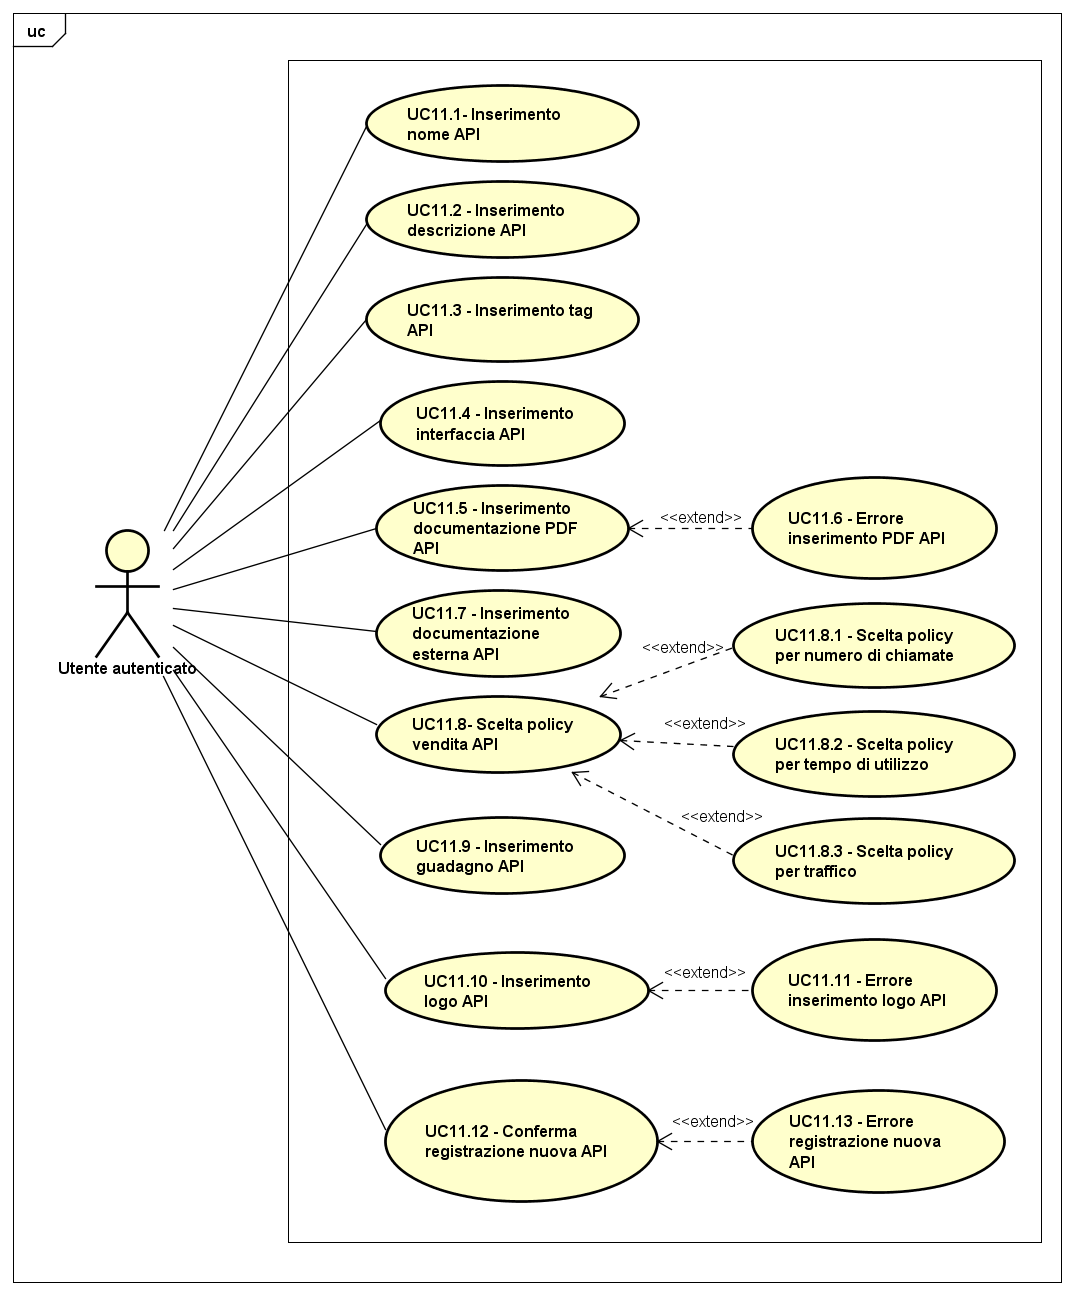
\includegraphics[scale=0.45]{UML/UC11.png}
	\caption{UC11: Registrazione nuova API}
\end{figure}

\begin{longtable}{ l | p{11cm}}
	\hline
	\rowcolor{Gray}
	\multicolumn{2}{c}{UC11 - Registrazione nuova API}\\
	\hline
	\textbf{Attori} & Sviluppatore \\
	\textbf{Descrizione} & L'attore registra una nuova API su API Market \\
	\textbf{Pre-Condizioni} & L'attore si trova nella schermata relativa alla registrazione di una nuova API \\
	\textbf{Post-Condizioni} & L'attore ha registrato una nuova API su API Market \\
	\textbf{Scenario Principale} & 
	\begin{enumerate*}[label=(\arabic*.),itemjoin={\newline}]
		\item L'attore può inserire il nome della nuova API (UC11.1)
		\item L'attore può inserire la descrizione della nuova API (UC11.2)
		\item L'attore può inserire la categoria della nuova API (UC11.3)
		\item L'attore può inserire l'interfaccia della nuova API (UC11.4)
		\item L'attore può inserire il file per la documentazione PDF della nuova API (UC11.5)
		\item L'attore può inserire il link per la documentazione esterna della nuova API (UC11.7)
		\item L'attore può scegliere la policy di vendita della nuova API (UC11.8)
		\item L'attore può inserire il guadagno netto desiderato per la nuova API (UC11.9)
		\item L'attore può inserire il file per il logo della nuova API (UC11.10)
		\item L'attore può confermare la registrazione della nuova API (UC11.12)
	\end{enumerate*}\\
	\textbf{Scenari Alternativi} & 
	\begin{enumerate*}[label=(\arabic*.),itemjoin={\newline}]
			\item L'attore può visualizzare un messaggio di errore riguardo al caricamento del file di documentazione PDF della nuova API, ed il caricamento del file non avviene (UC11.6)
			\item L'attore può scegliere la licenza API per numero di chiamate (UC11.8.1)
			\item L'attore può scegliere la licenza API per tempo di utilizzo (UC11.8.2)
			\item L'attore può scegliere la licenza API per traffico (UC11.8.3)
			\item L'attore può visualizzare un messaggio di errore riguardo al caricamento del file del logo della nuova API, ed il caricamento del file non avviene (UC11.11)
			\item L'attore, dopo aver confermato la registrazione della nuova API, può visualizzare un messaggio d'errore informativo e la registrazione non avviene (UC11.13)
	\end{enumerate*}\\
\end{longtable}

\subsubsection{Caso d'uso UC11.1: Inserimento nome API}
\label{UC11_1}

\begin{minipage}{\linewidth}
	\begin{tabular}{ l | p{11cm}}
		\hline
		\rowcolor{Gray}
		\multicolumn{2}{c}{UC11.1 - Inserimento nome API} \\
		\hline
		\textbf{Attori} & Sviluppatore \\
		\textbf{Descrizione} & L'attore inserisce il nome della nuova API \\
		\textbf{Pre-Condizioni} & L'attore si trova nella schermata relativa alla registrazione di una nuova API \\
		\textbf{Post-Condizioni} & L'attore ha inserito il nome della nuova API \\
		\textbf{Scenario Principale} & 
		\begin{enumerate*}[label=(\arabic*.),itemjoin={\newline}]
			\item L'attore può inserire il nome della nuova API
		\end{enumerate*}\\
	\end{tabular}
\end{minipage}

\subsubsection{Caso d'uso UC11.2: Inserimento descrizione API}
\label{UC11_2}

\begin{minipage}{\linewidth}
	\begin{tabular}{ l | p{11cm}}
		\hline
		\rowcolor{Gray}
		\multicolumn{2}{c}{UC11.2 - Inserimento descrizione API} \\
		\hline
		\textbf{Attori} & Sviluppatore \\
		\textbf{Descrizione} & L'attore inserisce la descrizione della nuova API \\
		\textbf{Pre-Condizioni} & L'attore si trova nella schermata relativa alla registrazione di una nuova API \\
		\textbf{Post-Condizioni} & L'attore ha inserito la descrizione della nuova API \\
		\textbf{Scenario Principale} & 
		\begin{enumerate*}[label=(\arabic*.),itemjoin={\newline}]
			\item L'attore può inserire la descrizione della nuova API
		\end{enumerate*}\\
	\end{tabular}
\end{minipage}

\subsubsection{Caso d'uso UC11.3: Inserimento categoria API}
\label{UC11_3}

\begin{minipage}{\linewidth}
	\begin{tabular}{ l | p{11cm}}
		\hline
		\rowcolor{Gray}
		\multicolumn{2}{c}{UC11.3 - Inserimento categoria API} \\
		\hline
		\textbf{Attori} & Sviluppatore \\
		\textbf{Descrizione} & L'attore inserisce la categoria della nuova API \\
		\textbf{Pre-Condizioni} & L'attore si trova nella schermata relativa alla registrazione di una nuova API \\
		\textbf{Post-Condizioni} & L'attore ha inserito la categoria della nuova API \\
		\textbf{Scenario Principale} & 
		\begin{enumerate*}[label=(\arabic*.),itemjoin={\newline}]
			\item L'attore può inserire la categoria della nuova API
		\end{enumerate*}\\
	\end{tabular}
\end{minipage}

\subsubsection{Caso d'uso UC11.4: Inserimento interfaccia API}
\label{UC11_4}

\begin{minipage}{\linewidth}
	\begin{tabular}{ l | p{11cm}}
		\hline
		\rowcolor{Gray}
		\multicolumn{2}{c}{UC11.4 - Inserimento interfaccia API} \\
		\hline
		\textbf{Attori} & Sviluppatore \\
		\textbf{Descrizione} & L'attore inserisce l'interfaccia della nuova API \\
		\textbf{Pre-Condizioni} & L'attore si trova nella schermata relativa alla registrazione di una nuova API \\
		\textbf{Post-Condizioni} & L'attore ha inserito l'interfaccia della nuova API \\
		\textbf{Scenario Principale} & 
		\begin{enumerate*}[label=(\arabic*.),itemjoin={\newline}]
			\item L'attore può inserire l'interfaccia della nuova API
		\end{enumerate*}\\
	\end{tabular}
\end{minipage}

\subsubsection{Caso d'uso UC11.5: Inserimento documentazione PDF API}
\label{UC11_5}

\begin{minipage}{\linewidth}
	\begin{tabular}{ l | p{11cm}}
		\hline
		\rowcolor{Gray}
		\multicolumn{2}{c}{UC11.5 - Inserimento documentazione PDF API} \\
		\hline
		\textbf{Attori} & Sviluppatore \\
		\textbf{Descrizione} & L'attore carica su API Market un file PDF contenente la documentazione PDF della nuova API \\
		\textbf{Pre-Condizioni} & L'attore si trova nella schermata relativa alla registrazione di una nuova API \\
		\textbf{Post-Condizioni} & L'attore ha caricato su API Market un file PDF contenente la documentazione PDF della nuova API \\
		\textbf{Scenario Principale} & 
		\begin{enumerate*}[label=(\arabic*.),itemjoin={\newline}]
			\item L'attore può caricare su API Market un file PDF contenente la documentazione PDF della nuova API
		\end{enumerate*}\\
		\textbf{Scenari Alternativi} & 
		\begin{enumerate*}[label=(\arabic*.),itemjoin={\newline}]
		\item L'attore può visualizzare un messaggio di errore (E.g: formato errato) ed il caricamento del file non avviene (UC11.10)
		\end{enumerate*}\\
	\end{tabular}
\end{minipage}

\subsubsection{Caso d'uso UC11.6: Errore inserimento PDF API}
\label{UC11_6}

\begin{minipage}{\linewidth}
	\begin{tabular}{ l | p{11cm}}
		\hline
		\rowcolor{Gray}
		\multicolumn{2}{c}{UC11.6 - Errore inserimento PDF API} \\
		\hline
		\textbf{Attori} & Sviluppatore \\
		\textbf{Descrizione} & L'attore visualizza un messaggio di errore e l'inserimento della documentazione PDF della nuova API non avviene \\
		\textbf{Pre-Condizioni} & L'attore ha cercato di caricare su API Market un file contenente la documentazione della nuova API ma si è verificato un errore \\
		\textbf{Post-Condizioni} & L'attore ha visualizzato un messaggio di errore \\
		\textbf{Scenario Principale} & 
		\begin{enumerate*}[label=(\arabic*.),itemjoin={\newline}]
			\item L'attore può visualizzare un messaggio di errore
		\end{enumerate*}\\
	\end{tabular}
\end{minipage}

\subsubsection{Caso d'uso UC11.7: Inserimento documentazione esterna API}
\label{UC11_7}

\begin{minipage}{\linewidth}
	\begin{tabular}{ l | p{11cm}}
		\hline
		\rowcolor{Gray}
		\multicolumn{2}{c}{UC11.7 - Inserimento documentazione esterna API} \\
		\hline
		\textbf{Attori} & Sviluppatore \\
		\textbf{Descrizione} & L'attore inserisce il link alla documentazione esterna della nuova API \\
		\textbf{Pre-Condizioni} & L'attore si trova nella schermata relativa alla registrazione di una nuova API \\
		\textbf{Post-Condizioni} & L'attore ha inserito il link alla documentazione esterna della nuova API \\
		\textbf{Scenario Principale} & 
		\begin{enumerate*}[label=(\arabic*.),itemjoin={\newline}]
			\item L'attore può inserire il link alla documentazione esterna della nuova API
		\end{enumerate*}\\
	\end{tabular}
\end{minipage}

\subsubsection{Caso d'uso UC11.8: Scelta policy vendita API}
\label{UC9_2}

\begin{minipage}{\linewidth}
	\begin{tabular}{ l | p{11cm}}
		\hline
		\rowcolor{Gray}
		\multicolumn{2}{c}{UC11.8.2 - Scelta policy vendita API} \\
		\hline
		\textbf{Attori} & Sviluppatore \\
		\textbf{Descrizione} & L'attore sceglie una policy di vendita per la nuova API \\
		\textbf{Pre-Condizioni} & L'attore si trova nella schermata di registrazione di una nuova API \\
		\textbf{Post-Condizioni} & L'attore ha scelto una policy di vendita per la nuova API \\
		\textbf{Scenario Principale} & 
		\begin{enumerate*}[label=(\arabic*.),itemjoin={\newline}]
			\item L'attore può scegliere una policy di vendita per la nuova API
		\end{enumerate*}\\
		\textbf{Scenari Alternativi} & 
		\begin{enumerate*}[label=(\arabic*.),itemjoin={\newline}]
			\item L'attore può scegliere la policy di vendita per numero di chiamate (UC11.8.1)
			\item L'attore può scegliere la policy di vendita per tempo di utilizzo (UC11.8.2)
			\item L'attore può scegliere la policy di vendita per traffico (UC11.8.3)	
		\end{enumerate*}\\
	\end{tabular}
\end{minipage}

\paragraph{Caso d'uso UC11.8.1: Scelta policy per numero di chiamate}
\label{UC11_8_1}

\begin{minipage}{\linewidth}
	\begin{tabular}{ l | p{11cm}}
		\hline
		\rowcolor{Gray}
		\multicolumn{2}{c}{UC11.8.1 - Scelta policy per numero di chiamate} \\
		\hline
		\textbf{Attori} & Sviluppatore \\
		\textbf{Descrizione} & L'attore sceglie la policy di vendita API per numero di chiamate \\
		\textbf{Pre-Condizioni} & L'attore si trova nella schermata di registrazione di una nuova API \\
		\textbf{Post-Condizioni} & L'attore ha scelto la policy di vendita API per numero di chiamate \\
		\textbf{Scenario Principale} & 
		\begin{enumerate*}[label=(\arabic*.),itemjoin={\newline}]
			\item L'attore può scegliere la policy di vendita API per numero di chiamate
		\end{enumerate*}\\
	\end{tabular}
\end{minipage}

\paragraph{Caso d'uso UC11.8.2: Scelta policy per tempo di utilizzo}
\label{UC11_8_2}

\begin{minipage}{\linewidth}
	\begin{tabular}{ l | p{11cm}}
		\hline
		\rowcolor{Gray}
		\multicolumn{2}{c}{UC11.8.2 - Scelta policy per tempo di utilizzo} \\
		\hline
		\textbf{Attori} & Sviluppatore \\
		\textbf{Descrizione} & L'attore sceglie la policy di vendita API per tempo di utilizzo \\
		\textbf{Pre-Condizioni} & L'attore si trova nella schermata di registrazione di una nuova API \\
		\textbf{Post-Condizioni} & L'attore ha scelto la policy di vendita API per tempo di utilizzo \\
		\textbf{Scenario Principale} & 
		\begin{enumerate*}[label=(\arabic*.),itemjoin={\newline}]
			\item L'attore può scegliere la policy di vendita API per tempo di utilizzo
		\end{enumerate*}\\
	\end{tabular}
\end{minipage}

\paragraph{Caso d'uso UC11.8.3: Scelta policy per traffico}
\label{UC11_8_3}

\begin{minipage}{\linewidth}
	\begin{tabular}{ l | p{11cm}}
		\hline
		\rowcolor{Gray}
		\multicolumn{2}{c}{UC11.8.3 - Scelta policy per traffico} \\
		\hline
		\textbf{Attori} & Sviluppatore \\
		\textbf{Descrizione} & L'attore sceglie la policy di vendita API per traffico \\
		\textbf{Pre-Condizioni} & L'attore si trova nella schermata di registrazione di una nuova API \\
		\textbf{Post-Condizioni} & L'attore ha scelto la policy di vendita API per traffico \\
		\textbf{Scenario Principale} & 
		\begin{enumerate*}[label=(\arabic*.),itemjoin={\newline}]
			\item L'attore può scegliere la policy di vendita API per traffico
		\end{enumerate*}\\
	\end{tabular}
\end{minipage}

\subsubsection{Caso d'uso UC11.9: Inserimento guadagno API}
\label{UC11_9}

\begin{minipage}{\linewidth}
	\begin{tabular}{ l | p{11cm}}
		\hline
		\rowcolor{Gray}
		\multicolumn{2}{c}{UC11.9 - Inserimento guadagno API} \\
		\hline
		\textbf{Attori} & Sviluppatore \\
		\textbf{Descrizione} & L'attore inserisce il guadagno netto desiderato per la nuova API \\
		\textbf{Pre-Condizioni} & L'attore si trova nella schermata relativa alla registrazione di una nuova API \\
		\textbf{Post-Condizioni} & L'attore ha inserito il guadagno netto desiderato per la nuova API \\
		\textbf{Scenario Principale} & 
		\begin{enumerate*}[label=(\arabic*.),itemjoin={\newline}]
			\item L'attore può inserire il guadagno netto desiderato per la nuova API
		\end{enumerate*}\\
	\end{tabular}
\end{minipage}

\subsubsection{Caso d'uso UC11.10: Inserimento logo API}
\label{UC11_10}

\begin{minipage}{\linewidth}
	\begin{tabular}{ l | p{11cm}}
		\hline
		\rowcolor{Gray}
		\multicolumn{2}{c}{UC11.10 - Inserimento logo API} \\
		\hline
		\textbf{Attori} & Sviluppatore \\
		\textbf{Descrizione} & L'attore carica su API Market un file contenente il logo per la nuova API \\
		\textbf{Pre-Condizioni} & L'attore si trova nella schermata relativa alla registrazione di una nuova API \\
		\textbf{Post-Condizioni} & L'attore ha caricato su API Market un file contenente il logo per la nuova API \\
		\textbf{Scenario Principale} & 
		\begin{enumerate*}[label=(\arabic*.),itemjoin={\newline}]
			\item L'attore può caricare su API Market un file contenente il logo per la nuova API
		\end{enumerate*}\\
		\textbf{Scenari Alternativi} & 
		\begin{enumerate*}[label=(\arabic*.),itemjoin={\newline}]
		\item L'attore può visualizzare un messaggio di errore (E.g: formato errato) ed il caricamento del file non avviene (UC11.11)
		\end{enumerate*}\\
	\end{tabular}
\end{minipage}

\subsubsection{Caso d'uso UC11.11: Errore inserimento logo API}
\label{UC11_11}

\begin{minipage}{\linewidth}
	\begin{tabular}{ l | p{11cm}}
		\hline
		\rowcolor{Gray}
		\multicolumn{2}{c}{UC11.11 - Errore inserimento logo API} \\
		\hline
		\textbf{Attori} & Sviluppatore \\
		\textbf{Descrizione} & L'attore visualizza un messaggio di errore e l'inserimento del logo per la nuova API non avviene \\
		\textbf{Pre-Condizioni} & L'attore ha cercato di caricare su API Market un file contenente il logo per la nuova API ma si è verificato un errore \\
		\textbf{Post-Condizioni} & L'attore ha visualizzato un messaggio di errore \\
		\textbf{Scenario Principale} & 
		\begin{enumerate*}[label=(\arabic*.),itemjoin={\newline}]
			\item L'attore può visualizzare un messaggio di errore (E.g: formato non valido)
		\end{enumerate*}\\
	\end{tabular}
\end{minipage}

\subsubsection{Caso d'uso UC11.12: Conferma registrazione nuova API}
\label{UC11_12}

\begin{minipage}{\linewidth}
	\begin{tabular}{ l | p{11cm}}
		\hline
		\rowcolor{Gray}
		\multicolumn{2}{c}{UC11.12 - Conferma registrazione nuova API} \\
		\hline
		\textbf{Attori} & Sviluppatore \\
		\textbf{Descrizione} & L'attore conferma la registrazione della nuova API \\
		\textbf{Pre-Condizioni} & L'attore si trova nella schermata relativa alla registrazione di una nuova API \\
		\textbf{Post-Condizioni} & L'attore ha confermato la registrazione della nuova API \\
		\textbf{Scenario Principale} & 
		\begin{enumerate*}[label=(\arabic*.),itemjoin={\newline}]
			\item L'attore può confermare la registrazione della nuova API, visualizzando un messaggio di successo e venendo reindirizzato alla schermata di visualizzazione API registrate (UC10)
		\end{enumerate*}\\
	\end{tabular}
\end{minipage}

\subsubsection{Caso d'uso UC11.13: Errore registrazione nuova API}
\label{UC11_13}

\begin{minipage}{\linewidth}
	\begin{tabular}{ l | p{11cm}}
		\hline
		\rowcolor{Gray}
		\multicolumn{2}{c}{UC11.13 - Errore registrazione nuova API} \\
		\hline
		\textbf{Attori} & Sviluppatore \\
		\textbf{Descrizione} & L'attore visualizza un messaggio di errore informativo e la registrazione della nuova API non avviene \\
		\textbf{Pre-Condizioni} & L'attore ha confermato la registrazione della una nuova API ma si è verificato un errore \\
		\textbf{Post-Condizioni} & L'attore ha visualizzato un messaggio di errore informativo \\
		\textbf{Scenario Principale} & 
		\begin{enumerate*}[label=(\arabic*.),itemjoin={\newline}]
			\item L'attore può visualizzare un messaggio di errore informativo e la registrazione della nuova API non avviene
		\end{enumerate*}\\
	\end{tabular}
\end{minipage}
\newpage
\subsection{Caso d'uso UC12: Gestione proprio profilo utente}
\label{UC12}
\begin{figure}[ht]
	\centering
	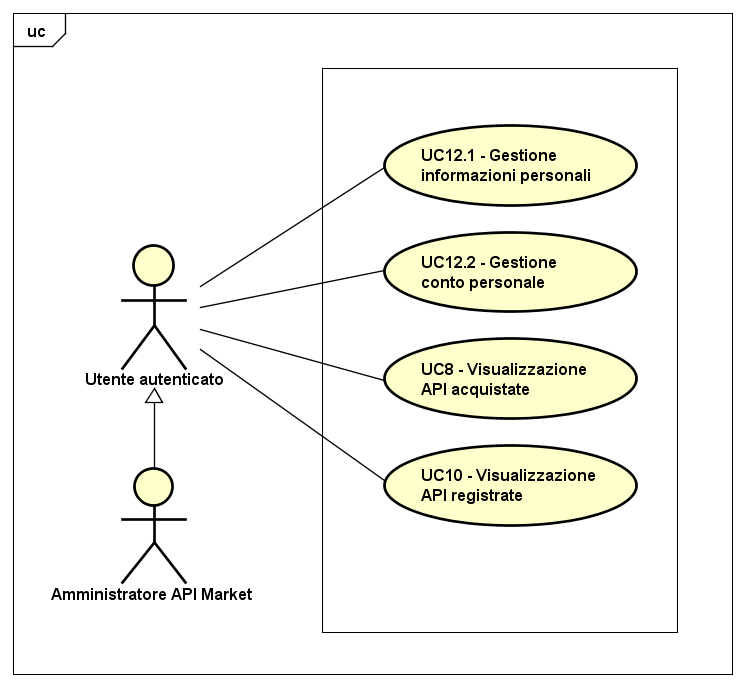
\includegraphics[scale=0.45]{UML/UC12.png}
	\caption{UC12 - Gestione proprio profilo utente}
\end{figure}

\begin{longtable}{ l | p{11cm}}
	\hline
	\rowcolor{Gray}
	\multicolumn{2}{c}{UC12 - Gestione proprio profilo utente} \\
	\hline
	\textbf{Attori} & Cliente, Sviluppatore \\
	\textbf{Descrizione} & L'attore visualizza e/o gestisce le informazioni del proprio profilo utente \\
	\textbf{Pre-Condizioni} & L'attore si trova nella schermata relativa alla gestione del proprio profilo utente \\
	\textbf{Post-Condizioni} & L'attore ha visualizzato e/o gestito le informazioni del proprio profilo utente \\
	\textbf{Scenario Principale} & 
	\begin{enumerate*}[label=(\arabic*.),itemjoin={\newline}]
		\item L'attore può gestire le proprie informazioni personali (UC12.1)
		\item L'attore può gestire il proprio conto utente (UC12.2)
		\item L'attore può visualizzare le API da lui acquistate (UC8)
		\item Lo sviluppatore può visualizzare le API da lui registrate (UC10)
	\end{enumerate*}\\
\end{longtable}

\newpage
\subsubsection{Caso d'uso UC12.1: Gestione informazioni personali}
\label{UC12_1}
\begin{figure}[ht]
	\centering
	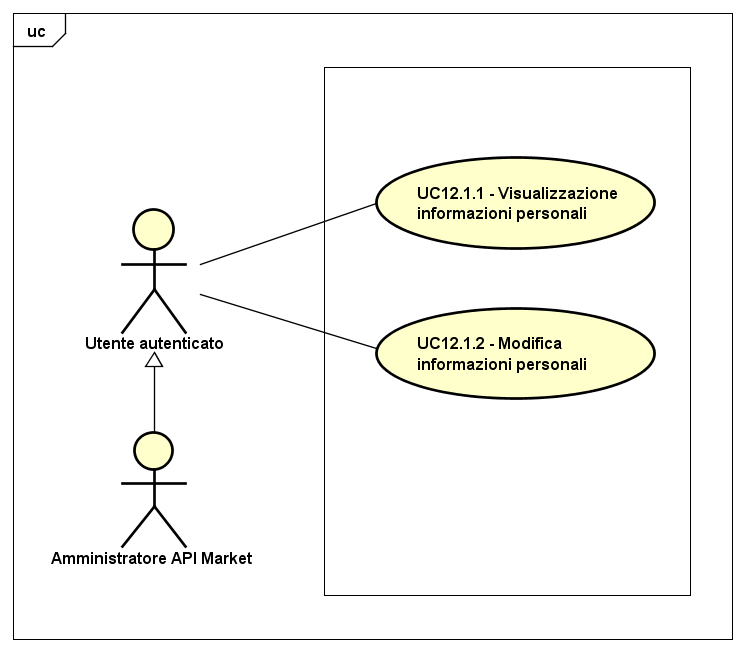
\includegraphics[scale=0.45]{UML/UC12_1.png}
	\caption{UC12.1: Gestione informazioni personali}
\end{figure}

\begin{minipage}{\linewidth}
	\begin{tabular}{ l | p{11cm}}
		\hline
		\rowcolor{Gray}
		\multicolumn{2}{c}{UC12.1 - Gestione informazioni personali} \\
		\hline
		\textbf{Attori} & Cliente \\
		\textbf{Descrizione} & L'attore visualizza e/o modifica le proprie informazioni personali \\
		\textbf{Pre-Condizioni} & L'attore si trova nella schermata relativa alla gestione del proprio profilo utente \\
		\textbf{Post-Condizioni} & L'attore ha visualizzato e/o modificato le proprie informazioni personali \\
		\textbf{Scenario Principale} & 
		\begin{enumerate*}[label=(\arabic*.),itemjoin={\newline}]
			\item L'attore può visualizzare le proprie informazioni personali (UC12.1.1)
			\item L'attore può modificare le proprie informazioni personali (UC12.1.2)
		\end{enumerate*}
	\end{tabular}
\end{minipage}

\newpage
\paragraph{Caso d'uso UC12.1.1: Visualizzazione informazioni personali}
\label{UC12_1_1}
\begin{figure}[ht]
	\centering
	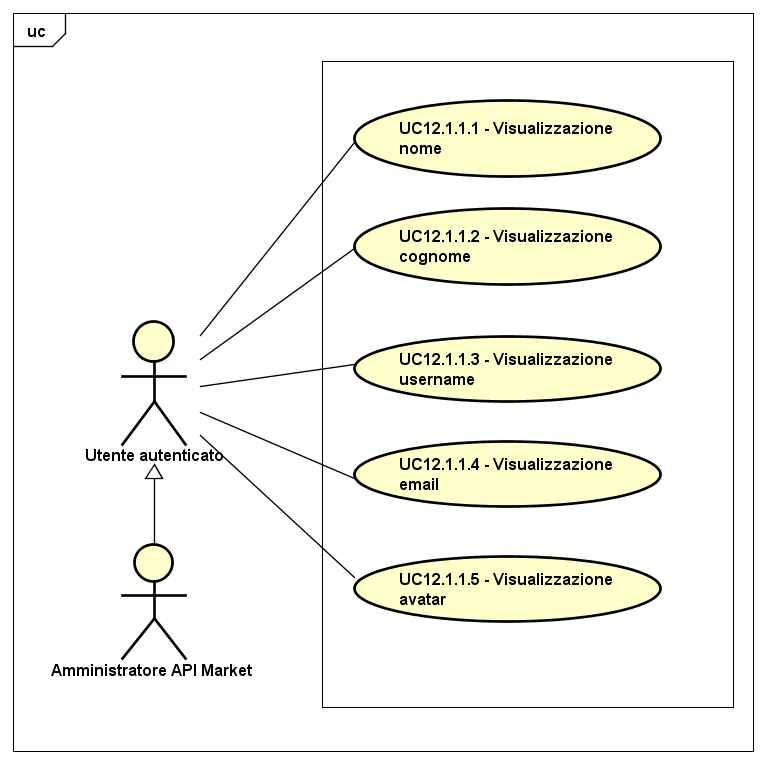
\includegraphics[scale=0.45]{UML/UC12_1_1.png}
	\caption{UC12.1.1: Visualizzazione informazioni personali}
\end{figure}

\begin{minipage}{\linewidth}
\begin{tabular}{ l | p{11cm}}
	\hline
	\rowcolor{Gray}
	\multicolumn{2}{c}{UC12.1.1 - Visualizzazione informazioni personali} \\
	\hline
	\textbf{Attori} & Cliente \\
	\textbf{Descrizione} & L'attore visualizza le proprie informazioni personali \\
	\textbf{Pre-Condizioni} & L'attore si trova nella schermata relativa alla gestione del proprio profilo utente \\
	\textbf{Post-Condizioni} & L'attore ha visualizzato le proprie informazioni personali \\
	\textbf{Scenario Principale} & 
	\begin{enumerate*}[label=(\arabic*.),itemjoin={\newline}]
		\item L'attore può visualizzare il proprio nome (UC12.1.1.1)
		\item L'attore può visualizzare il proprio cognome (UC12.1.1.2)
		\item L'attore può visualizzare il proprio username (UC12.1.1.3)
		\item L'attore può visualizzare la propria email (UC12.1.1.4)
		\item L'attore può visualizzare il proprio avatar (UC12.1.1.5)
		\item L'attore può visualizzare la tipologia del proprio account (UC12.1.1.6)
	\end{enumerate*}\\
\end{tabular}
\end{minipage}

\subparagraph{Caso d'uso UC12.1.1.1: Visualizzazione nome}
\label{UC12_1_1_1}

\begin{minipage}{\linewidth}
\begin{tabular}{ l | p{11cm}}
	\hline
	\rowcolor{Gray}
	\multicolumn{2}{c}{UC12.1.1.1 - Visualizzazione nome} \\
	\hline
	\textbf{Attori} & Cliente \\
	\textbf{Descrizione} & L'attore visualizzare il proprio nome \\
	\textbf{Pre-Condizioni} & L'attore si trova nella schermata relativa alla gestione delle informazioni personali \\
	\textbf{Post-Condizioni} & L'attore ha visualizzato il proprio nome \\
	\textbf{Scenario Principale} & 
	\begin{enumerate*}[label=(\arabic*.),itemjoin={\newline}]
		\item L'attore può visualizzare il proprio nome
	\end{enumerate*}
\end{tabular}
\end{minipage}

\subparagraph{Caso d'uso UC12.1.1.2: Visualizzazione cognome}
\label{UC12_1_1_2}

\begin{minipage}{\linewidth}
	\begin{tabular}{ l | p{11cm}}
		\hline
		\rowcolor{Gray}
		\multicolumn{2}{c}{UC12.1.1.2 - Visualizzazione cognome} \\
		\hline
		\textbf{Attori} & Cliente \\
		\textbf{Descrizione} & L'attore visualizzare il proprio cognome \\
	\textbf{Pre-Condizioni} & L'attore si trova nella schermata relativa alla gestione delle informazioni personali \\
	\textbf{Post-Condizioni} & L'attore ha visualizzato il proprio cognome \\
	\textbf{Scenario Principale} & 
	\begin{enumerate*}[label=(\arabic*.),itemjoin={\newline}]
		\item L'attore può visualizzare il proprio cognome
	\end{enumerate*}
	\end{tabular}
\end{minipage}

\subparagraph{Caso d'uso UC12.1.1.3: Visualizzazione username}
\label{UC12_1_1_3}

\begin{minipage}{\linewidth}
	\begin{tabular}{ l | p{11cm}}
		\hline
		\rowcolor{Gray}
		\multicolumn{2}{c}{UC12.1.1.3 - Visualizzazione username} \\
		\hline
		\textbf{Attori} & Cliente \\
		\textbf{Descrizione} & L'attore visualizzare il proprio username \\
	\textbf{Pre-Condizioni} & L'attore si trova nella schermata relativa alla gestione delle informazioni personali \\
	\textbf{Post-Condizioni} & L'attore ha visualizzato il proprio username \\
	\textbf{Scenario Principale} & 
	\begin{enumerate*}[label=(\arabic*.),itemjoin={\newline}]
		\item L'attore può visualizzare il proprio username
	\end{enumerate*}
	\end{tabular}
\end{minipage}

\subparagraph{Caso d'uso UC12.1.1.4: Visualizzazione email}
\label{UC12_1_1_4}

\begin{minipage}{\linewidth}
	\begin{tabular}{ l | p{11cm}}
		\hline
		\rowcolor{Gray}
		\multicolumn{2}{c}{UC12.1.1.4 - Visualizzazione email} \\
		\hline
		\textbf{Attori} & Cliente \\
		\textbf{Descrizione} & L'attore visualizzare la propria email \\
		\textbf{Pre-Condizioni} & L'attore si trova nella schermata relativa alla gestione delle informazioni personali \\
		\textbf{Post-Condizioni} & L'attore ha visualizzato la propria email \\
		\textbf{Scenario Principale} & 
		\begin{enumerate*}[label=(\arabic*.),itemjoin={\newline}]
			\item L'attore può visualizzare la propria email
		\end{enumerate*}
	\end{tabular}
\end{minipage}

\subparagraph{Caso d'uso UC12.1.1.5: Visualizzazione avatar}
\label{UC12_1_1_5}

\begin{minipage}{\linewidth}
	\begin{tabular}{ l | p{11cm}}
		\hline
		\rowcolor{Gray}
		\multicolumn{2}{c}{UC12.1.1.5 - Visualizzazione avatar} \\
		\hline
		\textbf{Attori} & Cliente \\
		\textbf{Descrizione} & L'attore visualizzare il proprio avatar \\
		\textbf{Pre-Condizioni} & L'attore si trova nella schermata relativa alla gestione delle informazioni personali \\
		\textbf{Post-Condizioni} & L'attore ha visualizzato il proprio avatar \\
		\textbf{Scenario Principale} & 
		\begin{enumerate*}[label=(\arabic*.),itemjoin={\newline}]
			\item L'attore può visualizzare il proprio avatar
		\end{enumerate*}
	\end{tabular}
\end{minipage}

\subparagraph{Caso d'uso UC12.1.1.6: Visualizzazione tipologia account}
\label{UC12_1_1_6}

\begin{minipage}{\linewidth}
	\begin{tabular}{ l | p{11cm}}
		\hline
		\rowcolor{Gray}
		\multicolumn{2}{c}{UC12.1.1.6 - Visualizzazione tipologia account} \\
		\hline
		\textbf{Attori} & Cliente \\
		\textbf{Descrizione} & L'attore visualizzare la tipologia del proprio account \\
		\textbf{Pre-Condizioni} & L'attore si trova nella schermata relativa alla gestione delle informazioni personali \\
		\textbf{Post-Condizioni} & L'attore ha visualizzato la tipologia del proprio account \\
		\textbf{Scenario Principale} & 
		\begin{enumerate*}[label=(\arabic*.),itemjoin={\newline}]
			\item L'attore può visualizzare la tipologia del proprio account
		\end{enumerate*}
	\end{tabular}
\end{minipage}

\newpage
\paragraph{Caso d'uso UC12.1.2: Modifica informazioni personali}
\label{UC12_1_2}
\begin{figure}[ht]
	\centering
	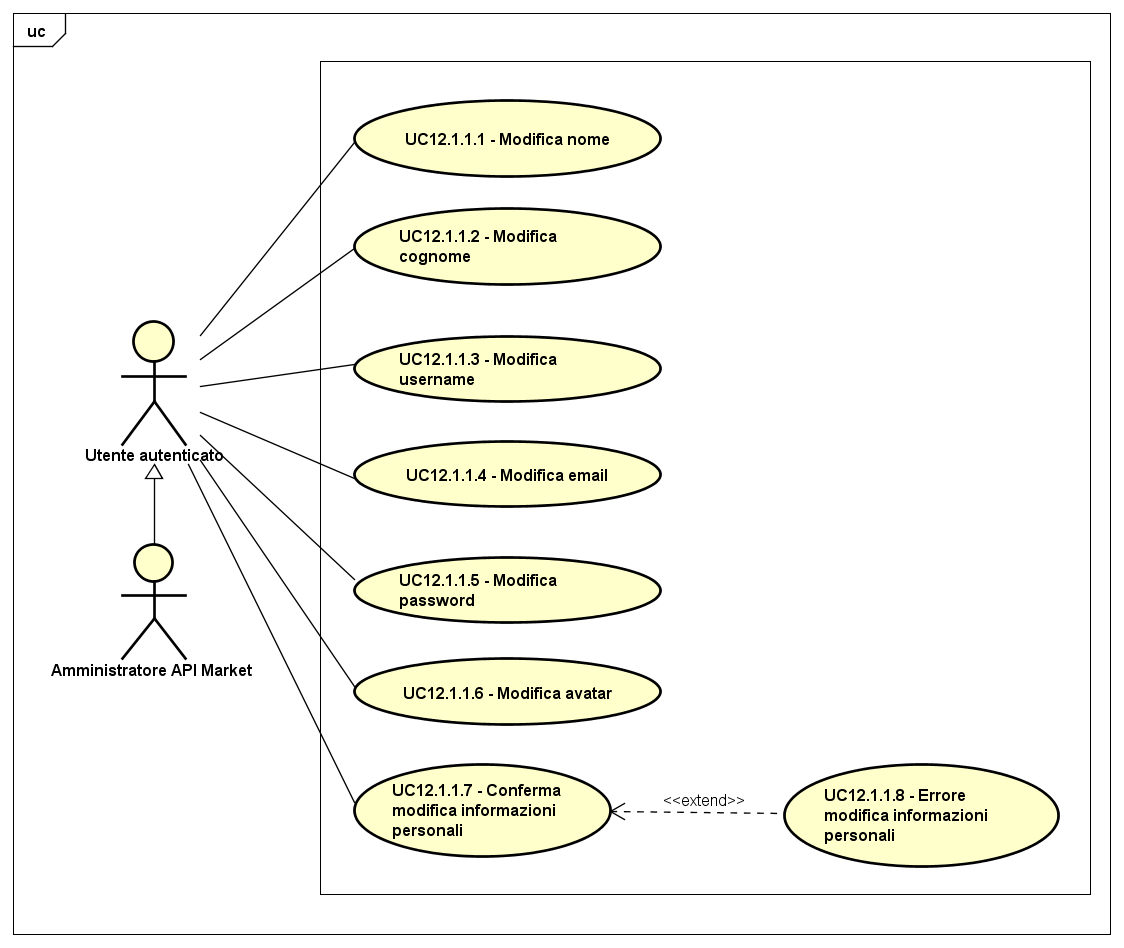
\includegraphics[scale=0.45]{UML/UC12_1_2.png}
	\caption{UC12.1.2: Modifica informazioni personali}
\end{figure}

\begin{tabular}{ l | p{11cm}}
	\hline
	\rowcolor{Gray}
	\multicolumn{2}{c}{UC12.1.2 - Modifica informazioni personali} \\
	\hline
	\textbf{Attori} & Cliente \\
	\textbf{Descrizione} & L'attore modifica le proprie informazioni personali \\
	\textbf{Pre-Condizioni} & L'attore si trova nella schermata relativa alla gestione del proprio profilo utente \\
	\textbf{Post-Condizioni} & L'attore ha modificato le proprie informazioni personali \\
	\textbf{Scenario Principale} & 
	\begin{enumerate*}[label=(\arabic*.),itemjoin={\newline}]
		\item L'attore può modificare il proprio nome (UC12.1.2.1)
		\item L'attore può modificare il proprio cognome (UC12.1.2.2)
		\item L'attore può modificare il proprio username (UC12.1.2.3)
		\item L'attore può modificare la propria email (UC12.1.2.4)
		\item L'attore può modificare la propria password (UC12.1.2.5)
		\item L'attore può modificare il proprio avatar (UC12.1.2.6)
		\item L'attore può confermare la modifica alle proprie informazioni personali (UC12.1.2.7)
	\end{enumerate*}\\
	\textbf{Scenari Alternativi} & 
	\begin{enumerate*}[label=(\arabic*.),itemjoin={\newline}]
		\item L'attore, dopo aver confermato le modifiche alle proprie informazioni personali, può visualizzare un messaggio di errore informativo (E.g: dati non validi, formati dei file errati), e le modifiche non avvengono (UC12.1.2.8)
	\end{enumerate*}\\
\end{tabular}

\subparagraph{Caso d'uso UC12.1.2.1: Modifica nome}
\label{UC12_1_2_1}

\begin{minipage}{\linewidth}
	\begin{tabular}{ l | p{11cm}}
		\hline
		\rowcolor{Gray}
		\multicolumn{2}{c}{UC12.1.2.1 - Modifica nome} \\
		\hline
		\textbf{Attori} & Cliente \\
		\textbf{Descrizione} & L'attore modifica il proprio nome \\
		\textbf{Pre-Condizioni} & L'attore si trova nella schermata relativa alla gestione delle informazioni personali \\
		\textbf{Post-Condizioni} & L'attore ha modificato il proprio nome \\
		\textbf{Scenario Principale} & 
		\begin{enumerate*}[label=(\arabic*.),itemjoin={\newline}]
			\item L'attore può modificare il proprio nome
		\end{enumerate*}
	\end{tabular}
\end{minipage}

\subparagraph{Caso d'uso UC12.1.2.2: Modifica cognome}
\label{UC12_1_2_2}

\begin{minipage}{\linewidth}
	\begin{tabular}{ l | p{11cm}}
		\hline
		\rowcolor{Gray}
		\multicolumn{2}{c}{UC12.1.2.2 - Modifica cognome} \\
		\hline
		\textbf{Attori} & Cliente \\
		\textbf{Descrizione} & L'attore modifica il proprio cognome \\
		\textbf{Pre-Condizioni} & L'attore si trova nella schermata relativa alla gestione delle informazioni personali \\
		\textbf{Post-Condizioni} & L'attore ha modificato il proprio cognome \\
		\textbf{Scenario Principale} & 
		\begin{enumerate*}[label=(\arabic*.),itemjoin={\newline}]
			\item L'attore può modificare il proprio cognome
		\end{enumerate*}
	\end{tabular}
\end{minipage}

\subparagraph{Caso d'uso UC12.1.2.3: Modifica username}
\label{UC12_1_2_3}

\begin{minipage}{\linewidth}
	\begin{tabular}{ l | p{11cm}}
		\hline
		\rowcolor{Gray}
		\multicolumn{2}{c}{UC12.1.2.3 - Modifica username} \\
		\hline
		\textbf{Attori} & Cliente \\
		\textbf{Descrizione} & L'attore modifica il proprio username \\
		\textbf{Pre-Condizioni} & L'attore si trova nella schermata relativa alla gestione delle informazioni personali \\
		\textbf{Post-Condizioni} & L'attore ha modificato il proprio username \\
		\textbf{Scenario Principale} & 
		\begin{enumerate*}[label=(\arabic*.),itemjoin={\newline}]
			\item L'attore può modificare il proprio username
		\end{enumerate*}
	\end{tabular}
\end{minipage}

\subparagraph{Caso d'uso UC12.1.2.4: Modifica email}
\label{UC12_1_2_4}

\begin{minipage}{\linewidth}
	\begin{tabular}{ l | p{11cm}}
		\hline
		\rowcolor{Gray}
		\multicolumn{2}{c}{UC12.1.2.4 - Modifica email} \\
		\hline
		\textbf{Attori} & Cliente \\
		\textbf{Descrizione} & L'attore modifica la propria email \\
		\textbf{Pre-Condizioni} & L'attore si trova nella schermata relativa alla gestione delle informazioni personali \\
		\textbf{Post-Condizioni} & L'attore ha modificato la propria email \\
		\textbf{Scenario Principale} & 
		\begin{enumerate*}[label=(\arabic*.),itemjoin={\newline}]
			\item L'attore può modificare la propria email
		\end{enumerate*}
	\end{tabular}
\end{minipage}

\subparagraph{Caso d'uso UC12.1.2.5: Modifica password}
\label{UC12_1_2_5}

\begin{minipage}{\linewidth}
	\begin{tabular}{ l | p{11cm}}
		\hline
		\rowcolor{Gray}
		\multicolumn{2}{c}{UC12.1.2.5 - Modifica password} \\
		\hline
		\textbf{Attori} & Cliente \\
		\textbf{Descrizione} & L'attore modifica la propria password \\
		\textbf{Pre-Condizioni} & L'attore si trova nella schermata relativa alla gestione delle informazioni personali \\
		\textbf{Post-Condizioni} & L'attore ha modificato la propria password \\
		\textbf{Scenario Principale} & 
		\begin{enumerate*}[label=(\arabic*.),itemjoin={\newline}]
			\item L'attore può modificare la propria password
		\end{enumerate*}
	\end{tabular}
\end{minipage}

\subparagraph{Caso d'uso UC12.1.2.6: Modifica avatar}
\label{UC12_1_2_6}

\begin{minipage}{\linewidth}
	\begin{tabular}{ l | p{11cm}}
		\hline
		\rowcolor{Gray}
		\multicolumn{2}{c}{UC12.1.2.6 - Modifica avatar} \\
		\hline
		\textbf{Attori} & Cliente \\
		\textbf{Descrizione} & L'attore modifica il proprio avatar \\
		\textbf{Pre-Condizioni} & L'attore si trova nella schermata relativa alla gestione delle informazioni personali \\
		\textbf{Post-Condizioni} & L'attore ha modificato il proprio avatar \\
		\textbf{Scenario Principale} & 
		\begin{enumerate*}[label=(\arabic*.),itemjoin={\newline}]
			\item L'attore può modificare il proprio avatar
		\end{enumerate*}
	\end{tabular}
\end{minipage}

\subparagraph{Caso d'uso UC12.1.2.7: Conferma modifica informazioni personali}
\label{UC12_1_2_7}

\begin{minipage}{\linewidth}
	\begin{tabular}{ l | p{11cm}}
		\hline
		\rowcolor{Gray}
		\multicolumn{2}{c}{UC12.1.2.7 - Conferma modifica informazioni personali} \\
		\hline
		\textbf{Attori} & Cliente \\
		\textbf{Descrizione} & L'attore conferma la modifica delle informazioni personali \\
		\textbf{Pre-Condizioni} & L'attore si trova nella schermata relativa alla gestione delle informazioni personali \\
		\textbf{Post-Condizioni} & L'attore ha confermato la modifica delle informazioni personali \\
		\textbf{Scenario Principale} & 
		\begin{enumerate*}[label=(\arabic*.),itemjoin={\newline}]
			\item L'attore può confermare la modifica delle informazioni personali, visualizzando un messaggio di successo
		\end{enumerate*}\\
	\end{tabular}
\end{minipage}

\subparagraph{Caso d'uso UC12.1.2.8: Errore modifica informazioni personali}
\label{UC12_1_2_8}

\begin{minipage}{\linewidth}
	\begin{tabular}{ l | p{11cm}}
		\hline
		\rowcolor{Gray}
		\multicolumn{2}{c}{UC12.1.2.8 - Errore modifica informazioni personali} \\
		\hline
		\textbf{Attori} & Cliente \\
		\textbf{Descrizione} & L'attore visualizza un messaggio di errore informativo e la modifica delle informazioni personali non avviene \\
		\textbf{Pre-Condizioni} & L'attore ha confermato la modifica delle informazioni personali ma si è verificato un errore \\
		\textbf{Post-Condizioni} & L'attore ha visualizzato un messaggio di errore informativo \\
		\textbf{Scenario Principale} & 
		\begin{enumerate*}[label=(\arabic*.),itemjoin={\newline}]
			\item L'attore può visualizzare un messaggio di errore informativo e la modifica delle informazioni personali non avviene
		\end{enumerate*}\\
	\end{tabular}
\end{minipage}

\newpage
\subsubsection{Caso d'uso UC12.2: Gestione conto personale}
\label{UC12_2}
\begin{figure}[ht]
	\centering
	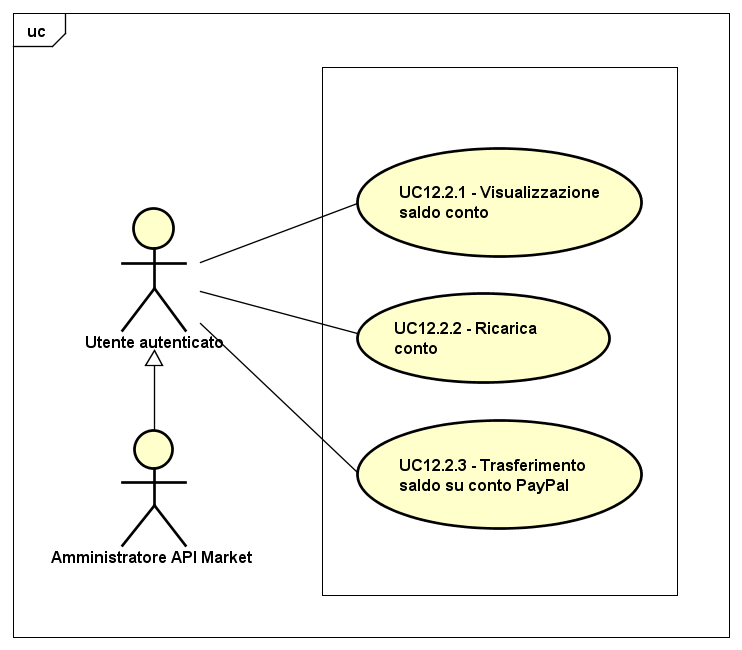
\includegraphics[scale=0.45]{UML/UC12_2.png}
	\caption{UC12.2: Gestione conto personale}
\end{figure}

\begin{minipage}{\linewidth}
	\begin{tabular}{ l | p{11cm}}
		\hline
		\rowcolor{Gray}
		\multicolumn{2}{c}{UC12.2 - Gestione conto personale} \\
		\hline
		\textbf{Attori} & Cliente \\
		\textbf{Descrizione} & L'attore visualizza le informazioni del proprio conto utente e/o effettua una ricarica su di esso \\
		\textbf{Pre-Condizioni} & L'attore si trova nella schermata relativa alla gestione del proprio profilo utente \\
		\textbf{Post-Condizioni} & L'attore ha visualizzato il saldo del proprio conto utente e/o effettuato una ricarica su di esso \\
		\textbf{Scenario Principale} & 
		\begin{enumerate*}[label=(\arabic*.),itemjoin={\newline}]
			\item L'attore può visualizzare il saldo corrente del proprio conto utente (UC12.2.1)
			\item L'attore può effettuare una ricarica sul proprio conto utente (UC12.2.2)
		\end{enumerate*}
	\end{tabular}
\end{minipage}

\paragraph{Caso d'uso UC12.2.1: Visualizzazione saldo conto}
\label{UC12_2_1}

\begin{minipage}{\linewidth}
	\begin{tabular}{ l | p{11cm}}
		\hline
		\rowcolor{Gray}
		\multicolumn{2}{c}{UC12.2.1 - Visualizzazione saldo conto} \\
		\hline
		\textbf{Attori} & Cliente \\
		\textbf{Descrizione} & L'attore visualizza il saldo corrente del proprio conto utente \\
		\textbf{Pre-Condizioni} & L'attore si trova nella schermata relativa alla gestione del proprio conto utente \\
		\textbf{Post-Condizioni} & L'attore ha visualizzato il saldo corrente del proprio conto utente \\
		\textbf{Scenario Principale} & 
		\begin{enumerate*}[label=(\arabic*.),itemjoin={\newline}]
			\item L'attore può visualizzare il saldo corrente del proprio conto utente
		\end{enumerate*}\\
	\end{tabular}
\end{minipage}

\paragraph{Caso d'uso UC12.2.2: Ricarica conto}
\label{UC12_2_2}
\begin{figure}[ht]
	\centering
	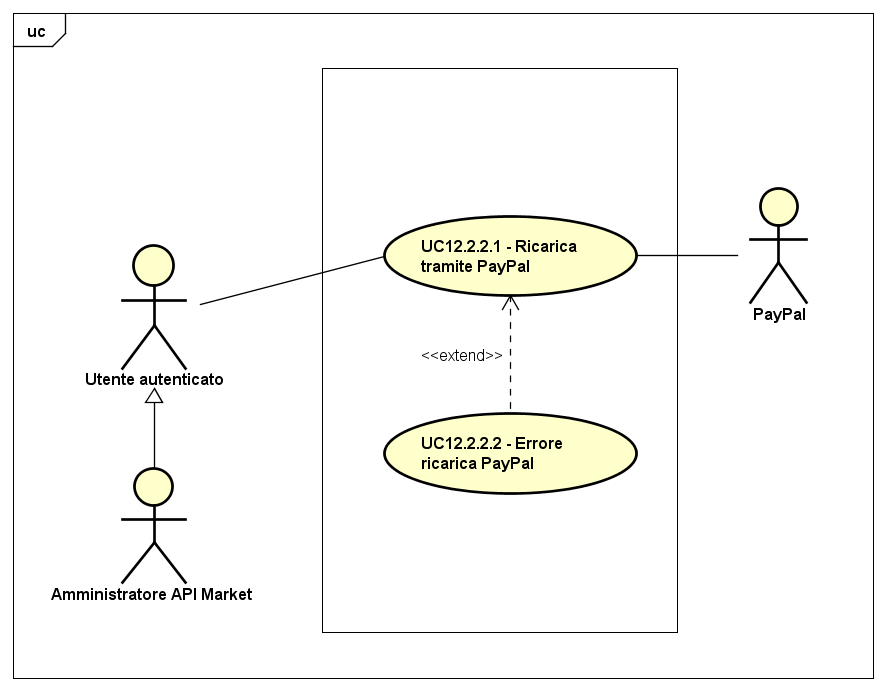
\includegraphics[scale=0.45]{UML/UC12_2_2.png}
	\caption{UC12.2.2: Ricarica conto}
\end{figure}

\begin{minipage}{\linewidth}
	\begin{tabular}{ l | p{11cm}}
		\hline
		\rowcolor{Gray}
		\multicolumn{2}{c}{UC12.2.2 - Ricarica conto} \\
		\hline
		\textbf{Attori} & Cliente, PayPal \\
		\textbf{Descrizione} & L'attore effettua una ricarica sul proprio conto utente \\
		\textbf{Pre-Condizioni} & L'attore si trova nella schermata relativa alla gestione del proprio conto utente \\
		\textbf{Post-Condizioni} & L'attore ha effettuato una ricarica sul proprio conto utente \\
		\textbf{Scenario Principale} & 
		\begin{enumerate*}[label=(\arabic*.),itemjoin={\newline}]
			\item L'attore può effettuare una ricarica tramite PayPal sul proprio conto utente (UC12.2.2.1)
		\end{enumerate*}\\
		\textbf{Scenari Alternativi} & 
		\begin{enumerate*}[label=(\arabic*.),itemjoin={\newline}]
			\item L'attore può visualizzare un messaggio di errore informativo (E.g: dati errati), e la ricarica tramite PayPal sul proprio conto utente non avviene (UC12.2.2.2)
		\end{enumerate*}\\
	\end{tabular}
\end{minipage}

\subparagraph{Caso d'uso UC12.2.2.1: Ricarica tramite PayPal}
\label{UC12_2_2_1}

\begin{minipage}{\linewidth}
	\begin{tabular}{ l | p{11cm}}
		\hline
		\rowcolor{Gray}
		\multicolumn{2}{c}{UC12.2.2.1 - Ricarica tramite PayPal} \\
		\hline
		\textbf{Attori} & Cliente, PayPal \\
		\textbf{Descrizione} & L'attore effettua una ricarica tramite PayPal sul proprio conto utente \\
		\textbf{Pre-Condizioni} & L'attore si trova nella schermata relativa alla ricarica del proprio conto utente \\
		\textbf{Post-Condizioni} & L'attore ha effettuato una ricarica tramite PayPal sul proprio conto utente \\
		\textbf{Scenario Principale} & 
		\begin{enumerate*}[label=(\arabic*.),itemjoin={\newline}]
			\item L'attore può effettuare una ricarica tramite PayPal sul proprio conto utente
		\end{enumerate*}\\
	\end{tabular}
\end{minipage}

\subparagraph{Caso d'uso UC12.2.2.2: Errore ricarica PayPal}
\label{UC12_2_2_2}

\begin{minipage}{\linewidth}
	\begin{tabular}{ l | p{11cm}}
		\hline
		\rowcolor{Gray}
		\multicolumn{2}{c}{UC12.2.2.2 - Errore ricarica PayPal} \\
		\hline
		\textbf{Attori} & Cliente, PayPal \\
		\textbf{Descrizione} & L'attore visualizza un messaggio di errore informativo e la ricarica tramite PayPal sul proprio conto utente non avviene \\
		\textbf{Pre-Condizioni} & L'attore ha confermato la ricarica tramite PayPal sul proprio conto utente ma si è verificato un errore \\
		\textbf{Post-Condizioni} & L'attore ha visualizzato un messaggio di errore informativo \\
		\textbf{Scenario Principale} & 
		\begin{enumerate*}[label=(\arabic*.),itemjoin={\newline}]
			\item L'attore può visualizzare un messaggio di errore informativo e la ricarica tramite PayPal sul proprio conto utente non avviene
		\end{enumerate*}\\
	\end{tabular}
\end{minipage}

\newpage
\subsubsection{Caso d'uso UC12.3: Visualizzazione storico transazioni}
\label{UC12_3}
\begin{figure}[ht]
	\centering
	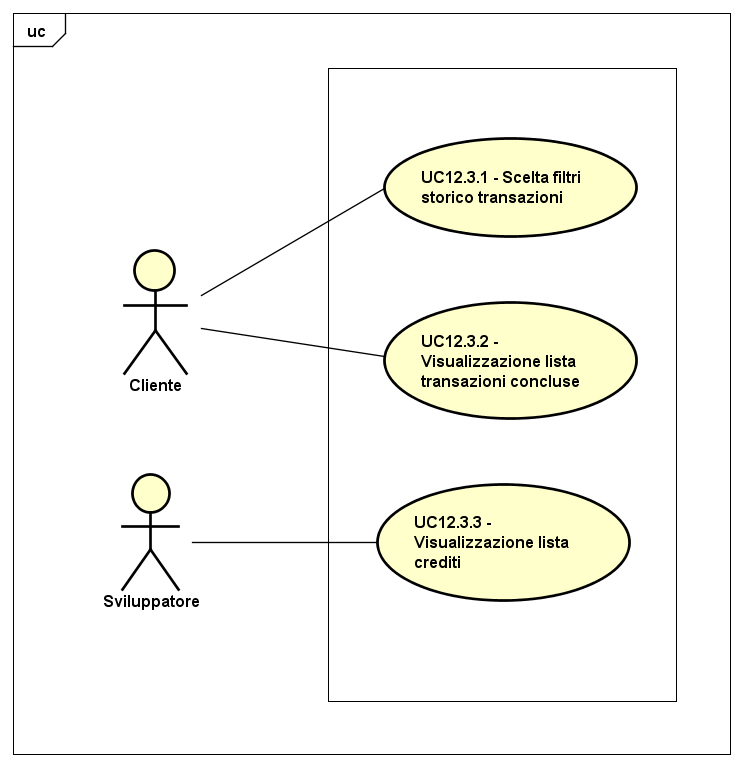
\includegraphics[scale=0.45]{UML/UC12_3.png}
	\caption{UC12.3: Visualizzazione storico transazioni}
\end{figure}

\begin{minipage}{\linewidth}
	\begin{tabular}{ l | p{11cm}}
		\hline
		\rowcolor{Gray}
		\multicolumn{2}{c}{UC12.3 - Visualizzazione storico transazioni} \\
		\hline
		\textbf{Attori} & Cliente, Sviluppatore \\
		\textbf{Descrizione} & L'attore visualizza lo storico delle proprie transazioni \\
		\textbf{Pre-Condizioni} & L'attore si trova nella schermata relativa alla gestione del proprio profilo utente \\
		\textbf{Post-Condizioni} & L'attore ha visualizzato lo storico delle proprie transazioni \\
		\textbf{Scenario Principale} & 
		\begin{enumerate*}[label=(\arabic*.),itemjoin={\newline}]
			\item L'attore può scegliere i filtri di visualizzazione (UC12.3.1)
			\item L'attore può visualizzare la lista delle proprie transazioni concluse (UC12.3.2)
			\item Lo sviluppatore può visualizzare la lista dei propri crediti (UC12.3.3)
		\end{enumerate*}
	\end{tabular}
\end{minipage}

\newpage
\paragraph{Caso d'uso UC12.3.1: Scelta filtri storico transazioni}
\label{UC12_3_1}
\begin{figure}[ht]
	\centering
	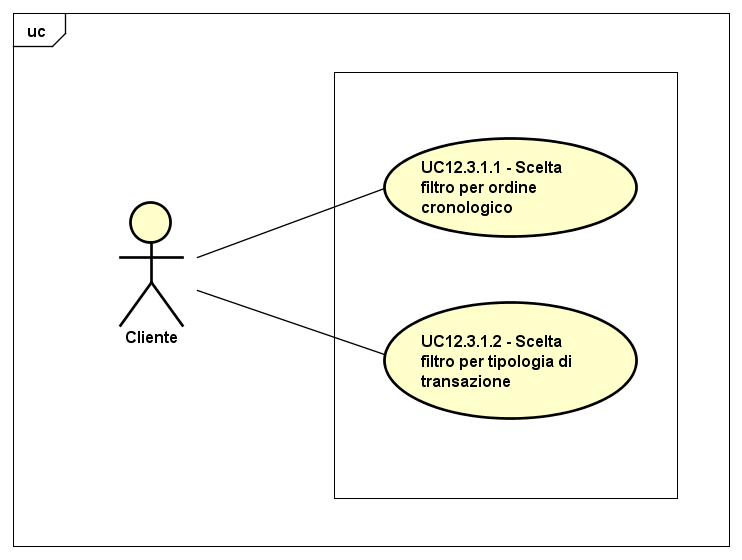
\includegraphics[scale=0.45]{UML/UC12_3_1.png}
	\caption{UC12.3.1: Scelta filtri storico transazioni}
\end{figure}

\begin{minipage}{\linewidth}
	\begin{tabular}{ l | p{11cm}}
		\hline
		\rowcolor{Gray}
		\multicolumn{2}{c}{UC12.3.1 - Scelta filtri storico transazioni} \\
		\hline
		\textbf{Attori} & Cliente \\
		\textbf{Descrizione} & L'attore scegliere i filtri per lo storico delle proprie transazioni \\
	\textbf{Pre-Condizioni} & L'attore si trova nella schermata relativa alla visualizzazione dello storico delle proprie transazioni \\
	\textbf{Post-Condizioni} & L'attore ha scelto i filtri per lo storico delle proprie transazioni \\
	\textbf{Scenario Principale} & 
	\begin{enumerate*}[label=(\arabic*.),itemjoin={\newline}]
		\item L'attore può scegliere il filtro per ordine cronologico (UC12.3.1.1)
		\item L'attore può scegliere il filtro per tipologia di transazione (UC12.3.1.2)
	\end{enumerate*}
	\end{tabular}
\end{minipage}

\subparagraph{Caso d'uso UC12.3.1.1: Scelta filtro per ordine cronologico}
\label{UC12_3_1_1}

\begin{minipage}{\linewidth}
	\begin{tabular}{ l | p{11cm}}
		\hline
		\rowcolor{Gray}
		\multicolumn{2}{c}{UC12.3.1.1 - Scelta filtro per ordine cronologico} \\
		\hline
		\textbf{Attori} & Cliente \\
		\textbf{Descrizione} & L'attore sceglie il filtro per ordine cronologico \\
	\textbf{Pre-Condizioni} & L'attore si trova nella schermata relativa alla visualizzazione dello storico delle proprie transazioni \\
	\textbf{Post-Condizioni} & L'attore ha scelto il filtro per ordine cronologico \\
	\textbf{Scenario Principale} & 
	\begin{enumerate*}[label=(\arabic*.),itemjoin={\newline}]
		\item L'attore può scegliere il filtro per ordine cronologico
	\end{enumerate*}
	\end{tabular}
\end{minipage}

\subparagraph{Caso d'uso UC12.3.1.2: Scelta filtro per tipologia di transazione}
\label{UC12_3_1_2}

\begin{minipage}{\linewidth}
	\begin{tabular}{ l | p{11cm}}
		\hline
		\rowcolor{Gray}
		\multicolumn{2}{c}{UC12.3.1.2 - Scelta filtro per tipologia di transazione} \\
		\hline
		\textbf{Attori} & Cliente \\
		\textbf{Descrizione} & L'attore sceglie il filtro per tipologia di transazione \\
	\textbf{Pre-Condizioni} & L'attore si trova nella schermata relativa alla visualizzazione dello storico delle proprie transazioni \\
	\textbf{Post-Condizioni} & L'attore ha scelto il filtro per tipologia di transazione \\
	\textbf{Scenario Principale} & 
	\begin{enumerate*}[label=(\arabic*.),itemjoin={\newline}]
		\item L'attore può scegliere il filtro per tipologia di transazione
	\end{enumerate*}
	\end{tabular}
\end{minipage}

\newpage
\paragraph{Caso d'uso UC12.3.2: Visualizzazione lista transazioni concluse}
\label{UC12_3_2}
\begin{figure}[ht]
	\centering
	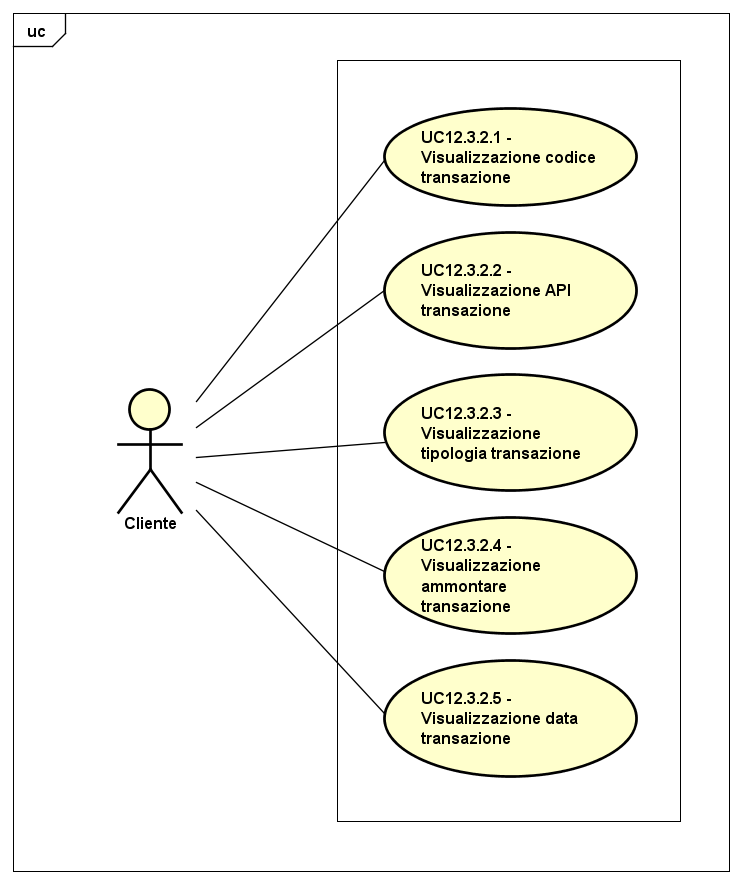
\includegraphics[scale=0.45]{UML/UC12_3_2.png}
	\caption{UC12.3.2: Visualizzazione lista transazioni concluse}
\end{figure}

\begin{minipage}{\linewidth}
	\begin{tabular}{ l | p{11cm}}
		\hline
		\rowcolor{Gray}
		\multicolumn{2}{c}{UC12.3.2 - Visualizzazione lista transazioni concluse} \\
		\hline
		\textbf{Attori} & Cliente \\
		\textbf{Descrizione} & L'attore visualizza la lista delle proprie transazioni \\
		\textbf{Pre-Condizioni} & L'attore si trova nella schermata relativa alla visualizzazione dello storico delle proprie transazioni \\
		\textbf{Post-Condizioni} & L'attore ha visualizzato la lista delle proprie transazioni \\
		\textbf{Scenario Principale} & 
		\begin{enumerate*}[label=(\arabic*.),itemjoin={\newline}]
			\item L'attore può visualizzare il codice della transazione (UC12.3.2.1)
			\item L'attore può visualizzare l'API di riferimento alla transazione (UC12.3.2.2)
			\item L'attore può visualizzare la tipologia della transazione (UC12.3.2.3)
			\item L'attore può visualizzare l'ammontare del denaro coinvolto nella transazione (UC12.3.2.4)
			\item L'attore può visualizzare la data della transazione (UC12.3.2.5)
		\end{enumerate*}\\
	\end{tabular}
\end{minipage}

\subparagraph{Caso d'uso UC12.3.2.1: Visualizzazione codice transazione}
\label{UC12_3_2_1}

\begin{minipage}{\linewidth}
	\begin{tabular}{ l | p{11cm}}
		\hline
		\rowcolor{Gray}
		\multicolumn{2}{c}{UC12.3.2.1 - Visualizzazione codice transazione} \\
		\hline
		\textbf{Attori} & Cliente \\
		\textbf{Descrizione} & L'attore visualizza il codice della propria transazione \\
	\textbf{Pre-Condizioni} & L'attore si trova nella schermata relativa alla visualizzazione dello storico delle proprie transazioni \\
	\textbf{Post-Condizioni} & L'attore ha visualizzato il codice della propria transazione \\
	\textbf{Scenario Principale} & 
	\begin{enumerate*}[label=(\arabic*.),itemjoin={\newline}]
		\item L'attore può visualizzare il codice della propria transazione
	\end{enumerate*}
	\end{tabular}
\end{minipage}

\subparagraph{Caso d'uso UC12.3.2.2: Visualizzazione API transazione}
\label{UC12_3_2_2}

\begin{minipage}{\linewidth}
	\begin{tabular}{ l | p{11cm}}
		\hline
		\rowcolor{Gray}
		\multicolumn{2}{c}{UC12.3.2.2 - Visualizzazione API transazione} \\
		\hline
		\textbf{Attori} & Cliente \\
		\textbf{Descrizione} & L'attore visualizza l'API di riferimento alla propria transazione \\
	\textbf{Pre-Condizioni} & L'attore si trova nella schermata relativa alla visualizzazione dello storico delle proprie transazioni \\
	\textbf{Post-Condizioni} & L'attore ha visualizzato l'API di riferimento alla propria transazione \\
	\textbf{Scenario Principale} & 
	\begin{enumerate*}[label=(\arabic*.),itemjoin={\newline}]
		\item L'attore può visualizzare l'API di riferimento alla propria transazione
	\end{enumerate*}
	\end{tabular}
\end{minipage}

\subparagraph{Caso d'uso UC12.3.2.3: Visualizzazione tipologia transazione}
\label{UC12_3_2_3}

\begin{minipage}{\linewidth}
	\begin{tabular}{ l | p{11cm}}
		\hline
		\rowcolor{Gray}
		\multicolumn{2}{c}{UC12.3.2.3 - Visualizzazione tipologia transazione} \\
		\hline
		\textbf{Attori} & Cliente \\
		\textbf{Descrizione} & L'attore visualizza la tipologia della propria transazione \\
	\textbf{Pre-Condizioni} & L'attore si trova nella schermata relativa alla visualizzazione dello storico delle proprie transazioni \\
	\textbf{Post-Condizioni} & L'attore ha visualizzato la tipologia della propria transazione \\
	\textbf{Scenario Principale} & 
	\begin{enumerate*}[label=(\arabic*.),itemjoin={\newline}]
		\item L'attore può visualizzare la tipologia della propria transazione
	\end{enumerate*}
	\end{tabular}
\end{minipage}

\subparagraph{Caso d'uso UC12.3.2.4: Visualizzazione ammontare transazione}
\label{UC12_3_2_4}

\begin{minipage}{\linewidth}
	\begin{tabular}{ l | p{11cm}}
		\hline
		\rowcolor{Gray}
		\multicolumn{2}{c}{UC12.3.2.4 - Visualizzazione ammontare transazione} \\
		\hline
		\textbf{Attori} & Cliente \\
		\textbf{Descrizione} & L'attore visualizza l'ammontare coinvolto nella propria transazione \\
	\textbf{Pre-Condizioni} & L'attore si trova nella schermata relativa alla visualizzazione dello storico delle proprie transazioni \\
	\textbf{Post-Condizioni} & L'attore ha visualizzato l'ammontare coinvolto nella propria transazione propria transazione \\
	\textbf{Scenario Principale} & 
	\begin{enumerate*}[label=(\arabic*.),itemjoin={\newline}]
		\item L'attore può visualizzare l'ammontare coinvolto nella propria transazione propria transazione
	\end{enumerate*}
	\end{tabular}
\end{minipage}

\subparagraph{Caso d'uso UC12.3.2.5: Visualizzazione data transazione}
\label{UC12_3_2_5}

\begin{minipage}{\linewidth}
	\begin{tabular}{ l | p{11cm}}
		\hline
		\rowcolor{Gray}
		\multicolumn{2}{c}{UC12.3.2.5 - Visualizzazione data transazione} \\
		\hline
		\textbf{Attori} & Cliente \\
		\textbf{Descrizione} & L'attore visualizza la data della propria transazione \\
	\textbf{Pre-Condizioni} & L'attore si trova nella schermata relativa alla visualizzazione dello storico delle proprie transazioni \\
	\textbf{Post-Condizioni} & L'attore ha visualizzato la data della propria transazione \\
	\textbf{Scenario Principale} & 
	\begin{enumerate*}[label=(\arabic*.),itemjoin={\newline}]
		\item L'attore può visualizzare la data della propria transazione
	\end{enumerate*}
	\end{tabular}
\end{minipage}

\newpage
\paragraph{Caso d'uso UC12.3.3: Visualizzazione lista credito}
\label{UC12_3_3}
\begin{figure}[ht]
	\centering
	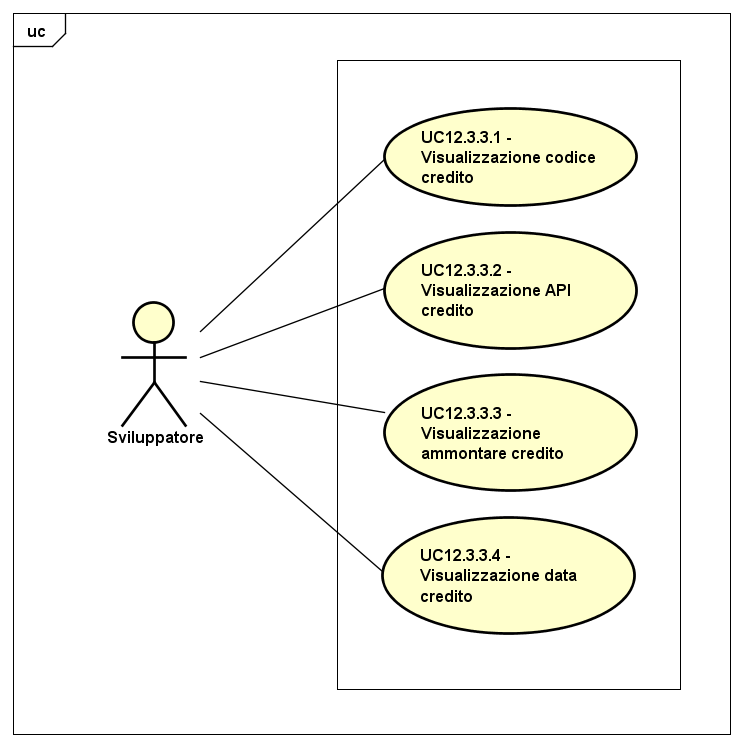
\includegraphics[scale=0.45]{UML/UC12_3_3.png}
	\caption{UC12.3.3: Visualizzazione lista credito}
\end{figure}

\begin{minipage}{\linewidth}
	\begin{tabular}{ l | p{11cm}}
		\hline
		\rowcolor{Gray}
		\multicolumn{2}{c}{UC12.3.3 - Visualizzazione lista credito} \\
		\hline
		\textbf{Attori} & Sviluppatore \\
		\textbf{Descrizione} & L'attore visualizza la lista dei propri crediti \\
		\textbf{Pre-Condizioni} & L'attore si trova nella schermata relativa alla visualizzazione dello storico delle proprie transazioni \\
		\textbf{Post-Condizioni} & L'attore ha visualizzato la lista dei propri crediti \\
		\textbf{Scenario Principale} & 
		\begin{enumerate*}[label=(\arabic*.),itemjoin={\newline}]
			\item L'attore può visualizzare il codice del credito (UC12.3.3.1)
			\item L'attore può visualizzare l'API di riferimento al credito (UC12.3.3.2)
			\item L'attore può visualizzare l'ammontare del credito accumulato per l'API di riferimento (UC12.3.3.3)
			\item L'attore può visualizzare la data del credito (UC12.3.3.4)
		\end{enumerate*}\\
	\end{tabular}
\end{minipage}

\subparagraph{Caso d'uso UC12.3.3.1: Visualizzazione codice credito}
\label{UC12_3_3_1}

\begin{minipage}{\linewidth}
	\begin{tabular}{ l | p{11cm}}
		\hline
		\rowcolor{Gray}
		\multicolumn{2}{c}{UC12.3.3.1 - Visualizzazione codice credito} \\
		\hline
		\textbf{Attori} & Sviluppatore \\
		\textbf{Descrizione} & L'attore visualizza il codice del proprio credito \\
	\textbf{Pre-Condizioni} & L'attore si trova nella schermata relativa alla visualizzazione dello storico delle proprie transazioni \\
	\textbf{Post-Condizioni} & L'attore ha visualizzato il codice del proprio credito \\
	\textbf{Scenario Principale} & 
	\begin{enumerate*}[label=(\arabic*.),itemjoin={\newline}]
		\item L'attore può visualizzare il codice del proprio credito
	\end{enumerate*}
	\end{tabular}
\end{minipage}

\subparagraph{Caso d'uso UC12.3.3.2: Visualizzazione API credito}
\label{UC12_3_3_2}

\begin{minipage}{\linewidth}
	\begin{tabular}{ l | p{11cm}}
		\hline
		\rowcolor{Gray}
		\multicolumn{2}{c}{UC12.3.3.2 - Visualizzazione API credito} \\
		\hline
		\textbf{Attori} & Sviluppatore \\
		\textbf{Descrizione} & L'attore visualizza l'API di riferimento al proprio credito \\
	\textbf{Pre-Condizioni} & L'attore si trova nella schermata relativa alla visualizzazione dello storico delle proprie transazioni \\
	\textbf{Post-Condizioni} & L'attore ha visualizzato l'API di riferimento al proprio credito \\
	\textbf{Scenario Principale} & 
	\begin{enumerate*}[label=(\arabic*.),itemjoin={\newline}]
		\item L'attore può visualizzare l'API di riferimento al proprio credito
	\end{enumerate*}
	\end{tabular}
\end{minipage}
	
\subparagraph{Caso d'uso UC12.3.3.3: Visualizzazione ammontare credito}
\label{UC12_3_3_3}

\begin{minipage}{\linewidth}
	\begin{tabular}{ l | p{11cm}}
		\hline
		\rowcolor{Gray}
		\multicolumn{2}{c}{UC12.3.3.3 - Visualizzazione ammontare credito} \\
		\hline
		\textbf{Attori} & Sviluppatore \\
		\textbf{Descrizione} & L'attore visualizza l'ammontare del proprio credito per l'API di riferimento \\
	\textbf{Pre-Condizioni} & L'attore si trova nella schermata relativa alla visualizzazione dello storico delle proprie transazioni \\
	\textbf{Post-Condizioni} & L'attore ha visualizzato ll'ammontare del proprio credito per l'API di riferimento \\
	\textbf{Scenario Principale} & 
	\begin{enumerate*}[label=(\arabic*.),itemjoin={\newline}]
		\item L'attore può visualizzare l'ammontare del proprio credito per l'API di riferimento
	\end{enumerate*}
	\end{tabular}
\end{minipage}

\subparagraph{Caso d'uso UC12.3.3.4: Visualizzazione data credito}
\label{UC12_3_3_4}

\begin{minipage}{\linewidth}
	\begin{tabular}{ l | p{11cm}}
		\hline
		\rowcolor{Gray}
		\multicolumn{2}{c}{UC12.3.3.4 - Visualizzazione data credito} \\
		\hline
		\textbf{Attori} & Sviluppatore \\
		\textbf{Descrizione} & L'attore visualizza la data del proprio credito per l'API di riferimento \\
	\textbf{Pre-Condizioni} & L'attore si trova nella schermata relativa alla visualizzazione dello storico delle proprie transazioni \\
	\textbf{Post-Condizioni} & L'attore ha visualizzato la data del proprio credito per l'API di riferimento \\
	\textbf{Scenario Principale} & 
	\begin{enumerate*}[label=(\arabic*.),itemjoin={\newline}]
		\item L'attore può visualizzare la data del proprio credito per l'API di riferimento
	\end{enumerate*}
	\end{tabular}
\end{minipage}
\newpage
\subsection{Caso d'uso UC13: Logout}
\label{UC13}

\begin{longtable}{ l | p{11cm}}
	\hline
	\rowcolor{Gray}
	\multicolumn{2}{c}{UC13 - Logout} \\
	\hline
	\textbf{Attori} & Cliente, Amministratore API Market \\
	\textbf{Descrizione} & L'attore effettua il logout, retrocedendo ad un utente non autenticato e venendo reindirizzato alla schermata iniziale \\
	\textbf{Pre-Condizioni} & L'attore si trova nella schermata iniziale dell'applicazione web \\
	\textbf{Post-Condizioni}& L'attore ha effettuato il logout, è stato retrocesso ad un utente non autenticato e reindirizzato alla schermata iniziale \\
	\textbf{Scenario Principale} & 
	\begin{enumerate*}[label=(\arabic*.),itemjoin={\newline}]
		\item L'attore può effettuare il logout, retrocedendo ad un utente non autenticato e venendo reindirizzato alla schermata iniziale (UC1)
	\end{enumerate*}\\
\end{longtable}
\newpage
\subsection{Caso d'uso UC14: Amministrazione applicazione web}
\label{UC14}
\begin{figure}[ht]
	\centering
	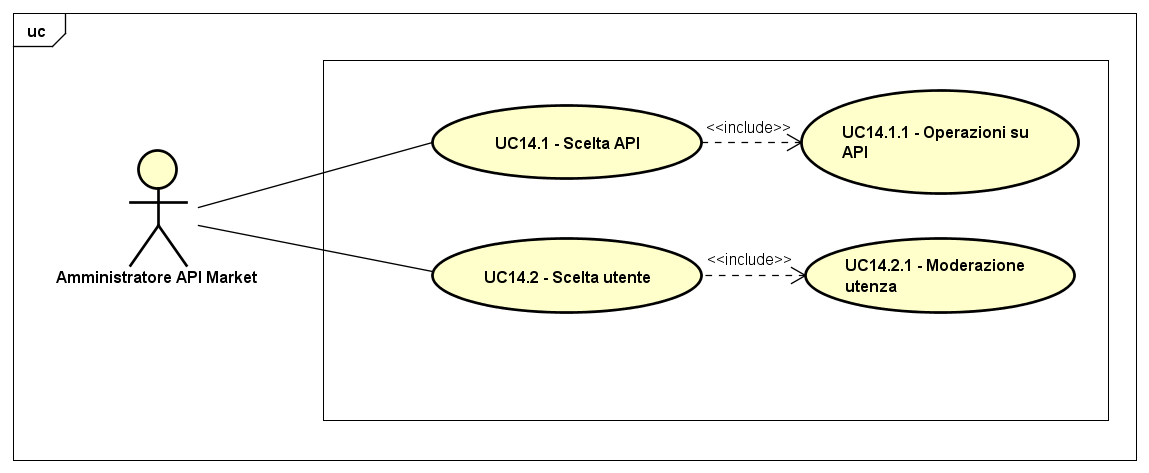
\includegraphics[scale=0.45]{UML/UC14.png}
	\caption{UC14 - Amministrazione applicazione web}
\end{figure}

\begin{longtable}{ l | p{11cm}}
	\hline
	\rowcolor{Gray}
	\multicolumn{2}{c}{UC14: Amministrazione applicazione web} \\
	\hline
	\textbf{Attori} & Amministratore API Market \\
	\textbf{Descrizione} & L'attore amministra l'applicazione web e/o consulta i dati di utilizzo avanzati \\
	\textbf{Pre-Condizioni} & L'attore si trova nella schermata iniziale dell'applicazione web \\
	\textbf{Post-Condizioni} & L'attore ha amministrato l'applicazione web e/o ha consultato i dati di utilizzo avanzati \\
	\textbf{Scenario Principale} & 
	\begin{enumerate*}[label=(\arabic*.),itemjoin={\newline}]
		\item L'attore può scegliere una API (UC14.1) per eseguire delle operazioni su di essa (UC14.1.1)
		\item L'attore può scegliere un utente (UC14.2) da moderare (UC14.2.1)
	\end{enumerate*}\\
\end{longtable}

\subsubsection{Caso d'uso UC14.1: Scelta API}
\label{UC14_1}

\begin{minipage}{\linewidth}
	\begin{tabular}{ l | p{11cm}}
		\hline
		\rowcolor{Gray}
		\multicolumn{2}{c}{UC14.1 - Scelta API} \\
		\hline
		\textbf{Attori} & Amministratore API Market \\
		\textbf{Descrizione} & L'attore sceglie una API su cui effettuare delle operazioni \\
		\textbf{Pre-Condizioni} & L'attore si trova nella schermata relativa all'amministrazione dell'applicazione web \\
		\textbf{Post-Condizioni} & L'attore ha scelto una API su cui effettuare delle operazioni \\
		\textbf{Scenario Principale} & 
		\begin{enumerate*}[label=(\arabic*.),itemjoin={\newline}]
			\item L'attore può scegliere una API su cui effettuare delle operazioni (UC14.1.1)
		\end{enumerate*}\\
	\end{tabular}
\end{minipage}

\newpage
\paragraph{Caso d'uso UC14.1.1: Operazioni su API}
\label{UC14_1_1}
\begin{figure}[ht]
	\centering
	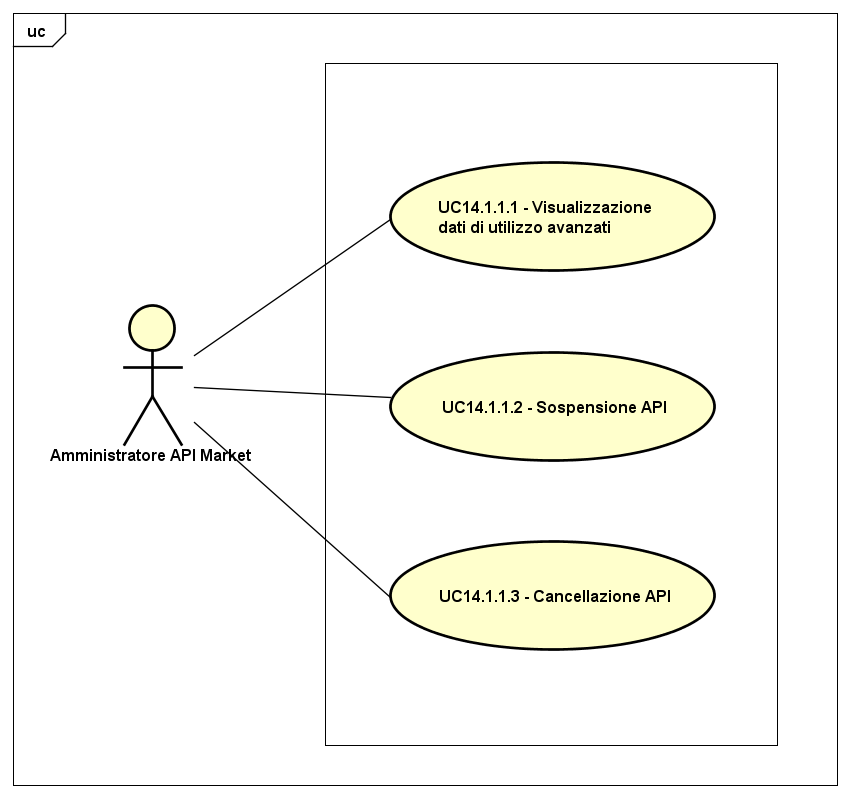
\includegraphics[scale=0.45]{UML/UC14_1_1.png}
	\caption{UC14.1.1: Operazioni su API}
\end{figure}

\begin{minipage}{\linewidth}
	\begin{tabular}{ l | p{11cm}}
		\hline
		\rowcolor{Gray}
		\multicolumn{2}{c}{UC14.1.1 - Operazioni su API} \\
		\hline
		\textbf{Attori} &  Amministratore API Market \\
		\textbf{Descrizione} & L'attore esegue le operazioni sull'API \\
		\textbf{Pre-Condizioni} & L'attore si trova nella schermata relativa all'amministrazione dell'applicazione web \\
		\textbf{Post-Condizioni} & L'attore ha concluso le operazioni sull'API \\
		\textbf{Scenario Principale} & 
		\begin{enumerate*}[label=(\arabic*.),itemjoin={\newline}]
			\item L'attore può visualizzare i dati avanzati dell'API (UC14.1.1.1)
			\item L'attore può sospendere il funzionamento dell'API (UC14.1.1.2)
			\item L'attore può cancellare l'API da API Market (UC14.1.1.3)
		\end{enumerate*}\\
	\end{tabular}
\end{minipage}

\newpage
\subparagraph{Caso d'uso UC14.1.1.1: Visualizzazione dati di utilizzo avanzati}
\label{UC14_1_1_1}
\begin{figure}[ht]
	\centering
	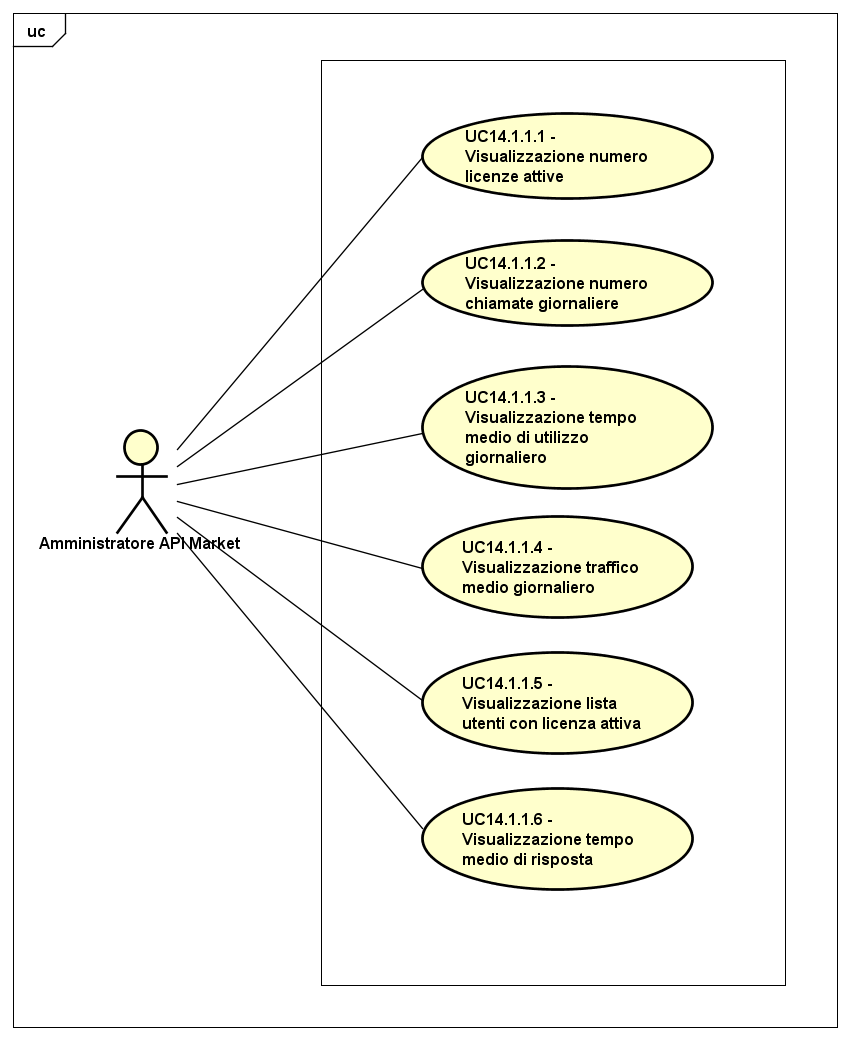
\includegraphics[scale=0.45]{UML/UC14_1_1_1.png}
	\caption{UC14.1.1: Visualizzazione dati di utilizzo avanzati}
\end{figure}

\begin{minipage}{\linewidth}
	\begin{tabular}{ l | p{11cm}}
		\hline
		\rowcolor{Gray}
		\multicolumn{2}{c}{UC14.1.1.1 - Visualizzazione dati di utilizzo avanzati} \\
		\hline
		\textbf{Attori} &  Amministratore API Market \\
		\textbf{Descrizione} & L'attore sceglie una API e ne visualizza i dati di utilizzo avanzati \\
		\textbf{Pre-Condizioni} & L'attore si trova nella schermata relativa all'amministrazione dell'applicazione web \\
		\textbf{Post-Condizioni} & L'attore ha scelto una API e ne ha visualizzato i dati di utilizzo avanzati \\
		\textbf{Scenario Principale} & 
		\begin{enumerate*}[label=(\arabic*.),itemjoin={\newline}]
			\item L'attore può visualizzare il numero di licenze attive dell'API scelta (UC14.1.1.1.1)
			\item L'attore può visualizzare il numero di chiamate giornaliere effettuate all'API scelta (UC14.1.1.1.2)
			\item L'attore può visualizzare il tempo medio di utilizzo giornaliero dell'API scelta (UC14.1.1.1.3)
			\item L'attore può visualizzare il traffico medio giornaliero dell'API scelta (UC14.1.1.1.4)
			\item L'attore può visualizzare la lista degli utenti con una licenza attiva per l'API scelta (UC14.1.1.1.5)
			\item L'attore può visualizzare il tempo medio di risposta dell'API scelta (UC14.1.1.1.6)
		\end{enumerate*}\\
	\end{tabular}
\end{minipage}

\subparagraph{Caso d'uso UC14.1.1.1.1: Visualizzazione numero licenze attive}
\label{UC14_1_1_1_1}

\begin{minipage}{\linewidth}
	\begin{tabular}{ l | p{11cm}}
		\hline
		\rowcolor{Gray}
		\multicolumn{2}{c}{UC14.1.1.1.1 - Visualizzazione numero licenze attive} \\
		\hline
		\textbf{Attori} & Amministratore API Market \\
		\textbf{Descrizione} & L'attore visualizza il numero di licenze attive per l'API scelta \\
		\textbf{Pre-Condizioni} & L'attore si trova nella schermata di visualizzazione dati di utilizzo API avanzati ed ha scelto una API \\
		\textbf{Post-Condizioni} & L'attore ha visualizzato il numero di licenze attive per l'API scelta \\
		\textbf{Scenario Principale} & 
		\begin{enumerate*}[label=(\arabic*.),itemjoin={\newline}]
			\item L'attore può visualizzare il numero di licenze attive per l'API scelta
		\end{enumerate*}\\
	\end{tabular}
\end{minipage}

\subparagraph{Caso d'uso UC14.1.1.1.2: Visualizzazione numero chiamate giornaliere}
\label{UC14_1_1_1_2}

\begin{minipage}{\linewidth}
	\begin{tabular}{ l | p{11cm}}
		\hline
		\rowcolor{Gray}
		\multicolumn{2}{c}{UC14.1.1.1.2 - Visualizzazione numero chiamate giornaliere} \\
		\hline
		\textbf{Attori} & Amministratore API Market \\
		\textbf{Descrizione} & L'attore visualizza il numero di chiamate giornaliere effettuate all'API scelta \\
		\textbf{Pre-Condizioni} & L'attore si trova nella schermata di visualizzazione dati di utilizzo API avanzati ed ha scelto una API \\
		\textbf{Post-Condizioni} & L'attore ha visualizzato il numero di chiamate giornaliere effettuate all'API scelta \\
		\textbf{Scenario Principale} & 
		\begin{enumerate*}[label=(\arabic*.),itemjoin={\newline}]
			\item L'attore può visualizzare il numero di chiamate giornaliere effettuate all'API scelta
		\end{enumerate*}\\
	\end{tabular}
\end{minipage}

\subparagraph{Caso d'uso UC14.1.1.1.3: Visualizzazione tempo medio di utilizzo giornaliero}
\label{UC14_1_1_1_3}

\begin{minipage}{\linewidth}
	\begin{tabular}{ l | p{11cm}}
		\hline
		\rowcolor{Gray}
		\multicolumn{2}{c}{14.1.1.1.3 - Visualizzazione tempo medio di utilizzo giornaliero} \\
		\hline
		\textbf{Attori} & Amministratore API Market \\
		\textbf{Descrizione} & L'attore visualizza il tempo medio di utilizzo giornaliero dell'API scelta \\
		\textbf{Pre-Condizioni} & L'attore si trova nella schermata di visualizzazione dati di utilizzo API avanzati ed ha scelto una API \\
		\textbf{Post-Condizioni} & L'attore ha visualizzato il tempo medio di utilizzo giornaliero dell'API scelta \\
		\textbf{Scenario Principale} & 
		\begin{enumerate*}[label=(\arabic*.),itemjoin={\newline}]
			\item L'attore può visualizzare il tempo medio di utilizzo giornaliero dell'API scelta
		\end{enumerate*}\\
	\end{tabular}
\end{minipage}

\subparagraph{Caso d'uso UC14.1.1.1.4: Visualizzazione traffico medio giornaliero}
\label{UC14_1_1_1_4}

\begin{minipage}{\linewidth}
	\begin{tabular}{ l | p{11cm}}
		\hline
		\rowcolor{Gray}
		\multicolumn{2}{c}{UC14.1.1.1.4 - Visualizzazione traffico medio giornaliero} \\
		\hline
		\textbf{Attori} & Amministratore API Market \\
		\textbf{Descrizione} & L'attore visualizza il traffico medio giornaliero dell'API scelta \\
		\textbf{Pre-Condizioni} & L'attore si trova nella schermata di visualizzazione dati di utilizzo API avanzati ed ha scelto una API \\
		\textbf{Post-Condizioni} & L'attore ha visualizzato il traffico medio giornaliero dell'API scelta \\
		\textbf{Scenario Principale} & 
		\begin{enumerate*}[label=(\arabic*.),itemjoin={\newline}]
			\item L'attore può visualizzare il traffico medio giornaliero dell'API scelta
		\end{enumerate*}\\
	\end{tabular}
\end{minipage}

\newpage
\subparagraph{Caso d'uso UC14.1.1.1.5: Visualizzazione utenti con licenza attiva}
\label{UC14_1_1_1_5}
\begin{figure}[ht]
	\centering
	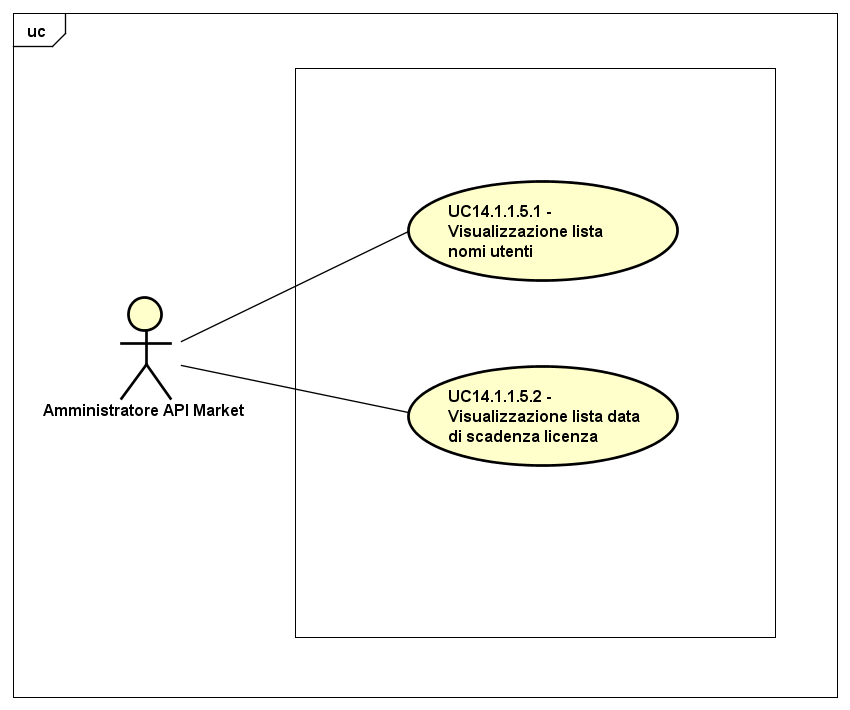
\includegraphics[scale=0.45]{UML/UC14_1_1_1_5.png}
	\caption{UC14.1.1.1.5: Visualizzazione utenti con licenza attiva}
\end{figure}

\begin{minipage}{\linewidth}
	\begin{tabular}{ l | p{11cm}}
		\hline
		\rowcolor{Gray}
		\multicolumn{2}{c}{UC14.1.1.1.5 - Visualizzazione utenti con licenza attiva} \\
		\hline
		\textbf{Attori} & Amministratore API Market \\
		\textbf{Descrizione} & L'attore ha scelto una API e visualizza una lista di utenti con licenze attive per l'API scelta\\
		\textbf{Pre-Condizioni} & L'attore si trova nella schermata di visualizzazione dati di utilizzo API avanzati ed ha scelto una API \\
		\textbf{Post-Condizioni} & L'attore ha visualizzato la lista di utenti con licenze attive per l'API scelta \\
		\textbf{Scenario Principale} & 
		\begin{enumerate*}[label=(\arabic*.),itemjoin={\newline}]
			\item L'attore può visualizzare il nome di ogni utente con licenza attiva per l'API scelta (UC14.1.1.1.5.1)
			\item L'attore può visualizzare la data di scadenza della licenza per ogni utente nella lista (UC14.1.1.1.5.2)
		\end{enumerate*}\\
	\end{tabular}
\end{minipage}

\subparagraph{Caso d'uso UC14.1.1.1.5.1: Visualizzazione lista nomi utenti}
\label{UC14_1_1_1_5_1}

\begin{minipage}{\linewidth}
	\begin{tabular}{ l | p{11cm}}
		\hline
		\rowcolor{Gray}
		\multicolumn{2}{c}{UC14.1.1.1.5.1 - Visualizzazione lista nomi utenti} \\
		\hline
		\textbf{Attori} & Amministratore API Market \\
		\textbf{Descrizione} & L'attore ha scelto una API e visualizza il nome dell'utente interessato\\
		\textbf{Pre-Condizioni} & L'attore si trova nella schermata di visualizzazione dati di utilizzo API avanzati ed ha scelto una API \\
		\textbf{Post-Condizioni} & L'attore ha visualizzato il nome per ogni utente della lista degli utenti con licenza attiva per l'API scelta \\
		\textbf{Scenario Principale} & 
		\begin{enumerate*}[label=(\arabic*.),itemjoin={\newline}]
			\item L'attore può visualizzare il nome per ogni utente della lista degli utenti con licenza attiva per l'API scelta
		\end{enumerate*}
	\end{tabular}
\end{minipage}

\subparagraph{Caso d'uso UC14.1.1.1.5.2: Visualizzazione lista scadenza licenza}
\label{UC14_1_1_1_5_2}

\begin{minipage}{\linewidth}
	\begin{tabular}{ l | p{11cm}}
		\hline
		\rowcolor{Gray}
		\multicolumn{2}{c}{UC14.1.1.1.5.2 -  Visualizzazione lista scadenza licenza} \\
		\hline
		\textbf{Attori} & Amministratore API Market \\
		\textbf{Descrizione} & L'attore ha scelto una API e visualizza il parametro di scadenza per ogni utente della lista degli utenti con licenza attiva per l'API scelta \\
		\textbf{Pre-Condizioni} & L'attore si trova nella schermata di visualizzazione dati di utilizzo API avanzati ed ha scelto una API \\
		\textbf{Post-Condizioni} & L'attore ha visualizzato il parametro di scadenza per ogni utente della lista degli utenti con licenza attiva per l'API scelta \\
		\textbf{Scenario Principale} & 
		\begin{enumerate*}[label=(\arabic*.),itemjoin={\newline}]
			\item L'attore può visualizzare il parametro di scadenza per ogni utente della lista degli utenti con licenza attiva per l'API scelta
		\end{enumerate*}
	\end{tabular}
\end{minipage}

\subparagraph{Caso d'uso UC14.1.1.1.6: Visualizzazione tempo medio di risposta}
\label{UC14_1_1_1_6}

\begin{minipage}{\linewidth}
	\begin{tabular}{ l | p{11cm}}
		\hline
		\rowcolor{Gray}
		\multicolumn{2}{c}{UC14.1.1.1.6 - Visualizzazione tempo medio di risposta} \\
		\hline
		\textbf{Attori} & Amministratore API Market \\
		\textbf{Descrizione} & L'attore ha scelto una API e visualizza il tempo medio di risposta dell'API scelta \\
		\textbf{Pre-Condizioni} & L'attore si trova nella schermata di visualizzazione dati di utilizzo API avanzati ed ha scelto una API \\
		\textbf{Post-Condizioni} & L'attore ha visualizzato il tempo medio di risposta dell'API scelta \\
		\textbf{Scenario Principale} & 
		\begin{enumerate*}[label=(\arabic*.),itemjoin={\newline}]
			\item L'attore può visualizzare il tempo medio di risposta dell'API scelta
		\end{enumerate*}\\
	\end{tabular}
\end{minipage}

\newpage
\subparagraph{Caso d'uso UC14.1.1.2: Sospensione API}
\label{UC14_1_1_2}
\begin{figure}[ht]
	\centering
	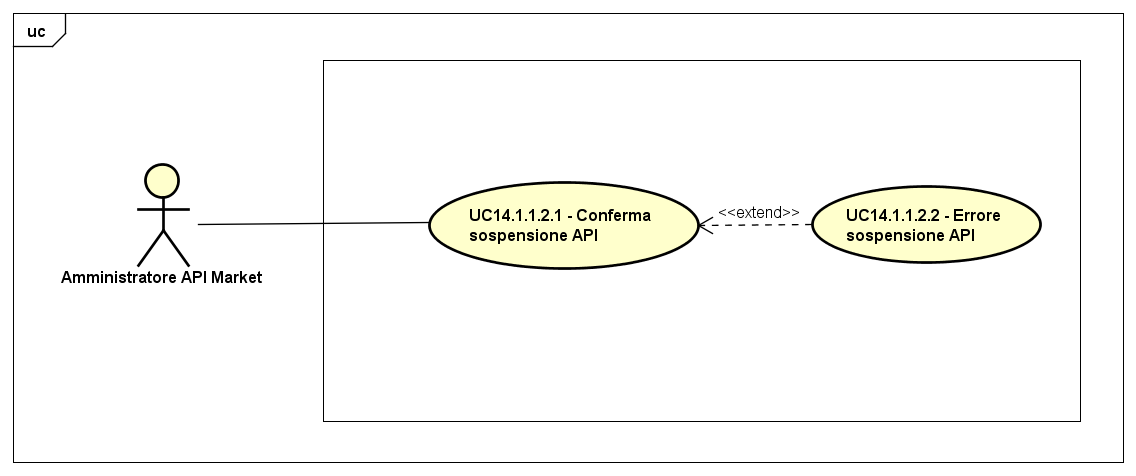
\includegraphics[scale=0.45]{UML/UC14_1_1_2.png}
	\caption{UC14.1.1.2: Sospensione API}
\end{figure}

\begin{minipage}{\linewidth}
	\begin{tabular}{ l | p{11cm}}
		\hline
		\rowcolor{Gray}
		\multicolumn{2}{c}{UC14.1.1.2 - Sospensione API} \\
		\hline
		\textbf{Attori} & Amministratore API Market \\
		\textbf{Descrizione} & L'attore sospende l'API scelta \\
		\textbf{Pre-Condizioni} & L'attore si trova nella schermata relativa alle operazioni su API ed ha scelto una API \\
		\textbf{Post-Condizioni} & L'attore ha sospeso l'API scelta \\
		\textbf{Scenario Principale} & 
		\begin{enumerate*}[label=(\arabic*.),itemjoin={\newline}]
			\item L'attore può confermare la sospensione dell'API scelta (UC14.1.1.2.1)
		\end{enumerate*}\\
		\textbf{Scenari Alternativi} & 
		\begin{enumerate*}[label=(\arabic*.),itemjoin={\newline}]
			\item L'attore, dopo aver confermato la sospensione dell'API scelta, può visualizzare un messaggio di errore informativo e la sospensione non avviene (UC14.1.1.2.2)
		\end{enumerate*}\\
	\end{tabular}
\end{minipage}

\subparagraph{Caso d'uso UC14.1.1.2.1: Conferma sospensione API}
\label{UC14_1_1_2_1}

\begin{minipage}{\linewidth}
	\begin{tabular}{ l | p{11cm}}
		\hline
		\rowcolor{Gray}
		\multicolumn{2}{c}{UC14.1.1.2.1 - Conferma sospensione API} \\
		\hline
		\textbf{Attori} & Amministratore API Market \\
		\textbf{Descrizione} & L'attore conferma la sospensione dell'utente scelto e visualizza un messaggio di successo \\
		\textbf{Pre-Condizioni} & L'attore si trova nella schermata relativa alle operazioni su API ed ha scelto una API \\
		\textbf{Post-Condizioni} & L'attore ha confermato la sospensione dell'API scelta \\
		\textbf{Scenario Principale} & 
		\begin{enumerate*}[label=(\arabic*.),itemjoin={\newline}]
			\item L'attore conferma la sospensione dell'API scelta e visualizza un messaggio di successo
		\end{enumerate*}\\
	\end{tabular}
\end{minipage}

\subparagraph{Caso d'uso UC14.1.1.2.2: Errore sospensione API}
\label{UC14_1_1_2_2}

\begin{minipage}{\linewidth}
	\begin{tabular}{ l | p{11cm}}
		\hline
		\rowcolor{Gray}
		\multicolumn{2}{c}{UC14.1.1.2.2 - Errore sospensione API} \\
		\hline
		\textbf{Attori} & Amministratore API Market \\
		\textbf{Descrizione} & L'attore visualizza un messaggio di errore informativo e la sospensione dell'API scelta non avviene \\
		\textbf{Pre-Condizioni} & L'attore ha confermato la sospensione dell'API scelta ma si è verificato un errore \\
		\textbf{Post-Condizioni} & L'attore ha visualizzato un messaggio di errore informativo \\
		\textbf{Scenario Principale} & 
		\begin{enumerate*}[label=(\arabic*.),itemjoin={\newline}]
			\item L'attore può visualizzare un messaggio di errore informativo e la sospensione dell'API scelta non avviene
		\end{enumerate*}\\
	\end{tabular}
\end{minipage}

\newpage
\subparagraph{Caso d'uso UC14.1.1.3: Cancellazione API}
\label{UC14_1_1_3}
\begin{figure}[ht]
	\centering
	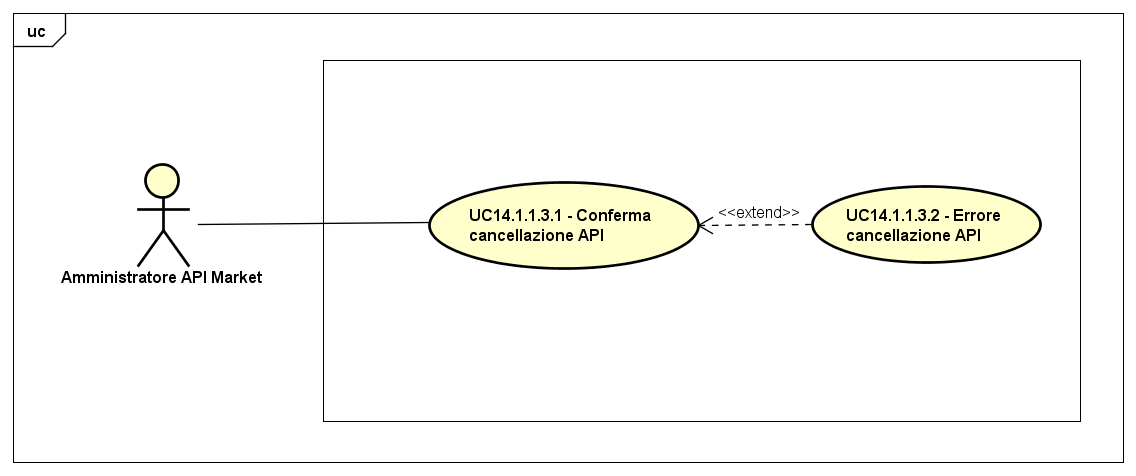
\includegraphics[scale=0.45]{UML/UC14_1_1_3.png}
	\caption{UC14.1.1.3: Cancellazione API}
\end{figure}

\begin{minipage}{\linewidth}
	\begin{tabular}{ l | p{11cm}}
		\hline
		\rowcolor{Gray}
		\multicolumn{2}{c}{UC14.1.1.3 - Cancellazione API} \\
		\hline
		\textbf{Attori} & Amministratore API Market \\
		\textbf{Descrizione} & L'attore cancella l'API scelta \\
		\textbf{Pre-Condizioni} & L'attore si trova nella schermata relativa alle operazioni su API ed ha scelto una API \\
		\textbf{Post-Condizioni} & L'attore ha cancellato l'API scelta \\
		\textbf{Scenario Principale} & 
		\begin{enumerate*}[label=(\arabic*.),itemjoin={\newline}]
			\item L'attore può confermare la cancellazione dell'API scelta (UC14.1.1.3.1)
		\end{enumerate*}\\
		\textbf{Scenari Alternativi} & 
		\begin{enumerate*}[label=(\arabic*.),itemjoin={\newline}]
			\item L'attore, dopo aver confermato la cancellazione dell'API scelta, può visualizzare un messaggio di errore informativo e la cancellazione non avviene (UC14.1.1.3.2)
			\item L'attore, dopo aver confermato la cancellazione dell'API scelta, può visualizzare un messaggio di avviso (E.g: Almeno una chiave API è ancora valida) e può riconfermare la cancellazione oppure abbandonarla (UC14.1.1.3.3)
		\end{enumerate*}\\
	\end{tabular}
\end{minipage}

\subparagraph{Caso d'uso UC14.1.1.3.1: Conferma cancellazione API}
\label{UC14_1_1_3_1}

\begin{minipage}{\linewidth}
	\begin{tabular}{ l | p{11cm}}
		\hline
		\rowcolor{Gray}
		\multicolumn{2}{c}{UC14.1.1.3.1 - Conferma cancellazione API} \\
		\hline
		\textbf{Attori} & Amministratore API Market \\
		\textbf{Descrizione} & L'attore conferma la cancellazione dell'utente scelto e visualizza un messaggio di successo \\
		\textbf{Pre-Condizioni} & L'attore si trova nella schermata relativa alle operazioni su API ed ha scelto una API \\
		\textbf{Post-Condizioni} & L'attore ha confermato la cancellazione dell'API scelta \\
		\textbf{Scenario Principale} & 
		\begin{enumerate*}[label=(\arabic*.),itemjoin={\newline}]
			\item L'attore conferma la cancellazione dell'API scelta e visualizza un messaggio di successo
		\end{enumerate*}\\
	\end{tabular}
\end{minipage}

\subparagraph{Caso d'uso UC14.1.1.3.2: Errore cancellazione API}
\label{UC14_1_1_3_2}

\begin{minipage}{\linewidth}
	\begin{tabular}{ l | p{11cm}}
		\hline
		\rowcolor{Gray}
		\multicolumn{2}{c}{UC14.1.1.3.2 - Errore cancellazione API} \\
		\hline
		\textbf{Attori} & Amministratore API Market \\
		\textbf{Descrizione} & L'attore visualizza un messaggio di errore informativo e la cancellazione dell'API scelta non avviene \\
		\textbf{Pre-Condizioni} & L'attore ha confermato la cancellazione dell'API scelta ma si è verificato un errore \\
		\textbf{Post-Condizioni} & L'attore ha visualizzato un messaggio di errore informativo \\
		\textbf{Scenario Principale} & 
		\begin{enumerate*}[label=(\arabic*.),itemjoin={\newline}]
			\item L'attore può visualizzare un messaggio di errore informativo e la cancellazione dell'API scelta non avviene
		\end{enumerate*}\\
	\end{tabular}
\end{minipage}

\subparagraph{Caso d'uso UC14.1.1.3.3: Avviso cancellazione API}
\label{UC14_1_1_3_3}

\begin{minipage}{\linewidth}
	\begin{tabular}{ l | p{11cm}}
		\hline
		\rowcolor{Gray}
		\multicolumn{2}{c}{UC14.1.1.3.3 - Avviso cancellazione API} \\
		\hline
		\textbf{Attori} & Amministratore API Market \\
		\textbf{Descrizione} & L'attore visualizza un messaggio di avviso e sceglie se riconfermare la cancellazione dell'API \\
		\textbf{Pre-Condizioni} & L'attore ha confermato la cancellazione dell'API scelta ma si è verificato un errore \\
		\textbf{Post-Condizioni} & L'attore ha visualizzato un messaggio di avviso ed ha scelto se riconfermare la cancellazione dell'API \\
		\textbf{Scenario Principale} & 
		\begin{enumerate*}[label=(\arabic*.),itemjoin={\newline}]
			\item L'attore può visualizzare un messaggio di avviso e scegliere se riconfermare la cancellazione dell'API
		\end{enumerate*}\\
	\end{tabular}
\end{minipage}

\subsubsection{Caso d'uso UC14.2: Scelta utente}
\label{UC14_2}

\begin{minipage}{\linewidth}
	\begin{tabular}{ l | p{11cm}}
		\hline
		\rowcolor{Gray}
		\multicolumn{2}{c}{UC14.2 - Scelta utente} \\
		\hline
		\textbf{Attori} & Amministratore API Market \\
		\textbf{Descrizione} & L'attore sceglie un utente da moderare \\
		\textbf{Pre-Condizioni} & L'attore si trova nella schermata relativa all'amministrazione dell'applicazione web \\
		\textbf{Post-Condizioni} & L'attore ha scelto un utente da moderare \\
		\textbf{Scenario Principale} & 
		\begin{enumerate*}[label=(\arabic*.),itemjoin={\newline}]
			\item L'attore può scegliere un utente da moderare (UC14.2.1)
		\end{enumerate*}\\
	\end{tabular}
\end{minipage}

\newpage
\paragraph{Caso d'uso UC14.2.1: Moderazione utenza}
\label{UC14_2_1}
\begin{figure}[ht]
	\centering
	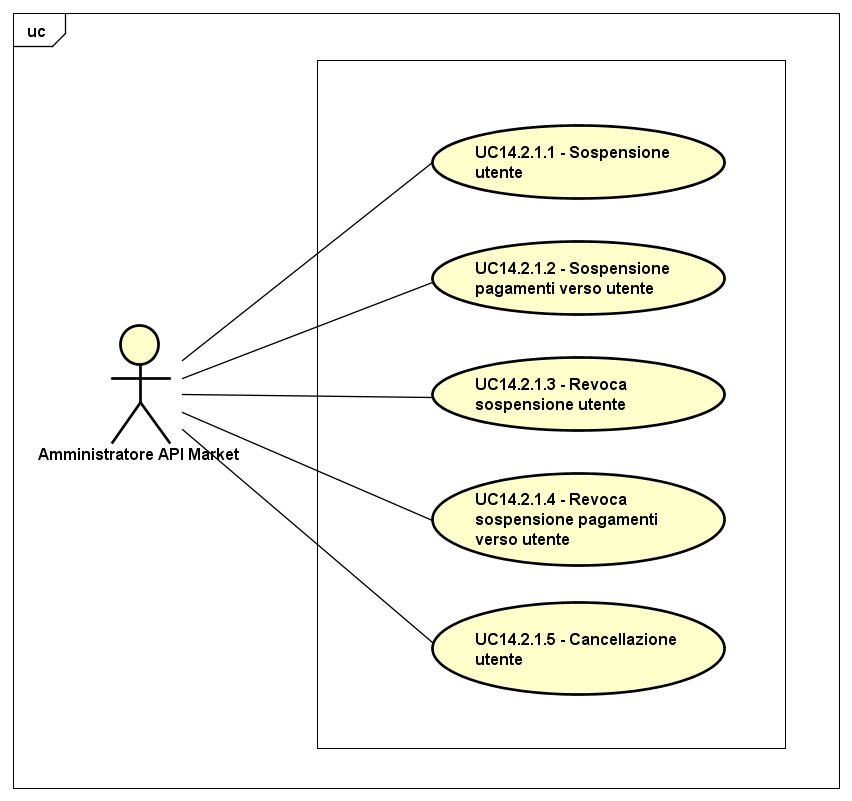
\includegraphics[scale=0.45]{UML/UC14_2_1.png}
	\caption{UC14.2.1: Moderazione utenza}
\end{figure}

\begin{minipage}{\linewidth}
	\begin{tabular}{ l | p{11cm}}
		\hline
		\rowcolor{Gray}
		\multicolumn{2}{c}{UC14.2.1 - Moderazione utenza} \\
		\hline
		\textbf{Attori} &  Amministratore API Market \\
		\textbf{Descrizione} & L'attore attua l'opera di moderazione \\
		\textbf{Pre-Condizioni} & L'attore si trova nella schermata relativa all'amministrazione dell'applicazione web \\
		\textbf{Post-Condizioni} & L'attore ha concluso l'opera di moderazione \\
		\textbf{Scenario Principale} & 
		\begin{enumerate*}[label=(\arabic*.),itemjoin={\newline}]
			\item L'attore può sospendere l'utente scelto (UC14.2.1.1)
			\item L'attore può sospendere i pagamenti verso l'utente scelto (UC14.2.1.2)
			\item L'attore può revocare la sospensione dell'utente scelto (UC14.2.1.3)
			\item L'attore può revocare la sospensione dei pagamenti verso l'utente scelto (UC14.2.1.4)
		\end{enumerate*}\\
	\end{tabular}
\end{minipage}

\newpage
\subparagraph{Caso d'uso UC14.2.1.1: Sospensione utente}
\label{UC14_2_1_1}
\begin{figure}[ht]
	\centering
	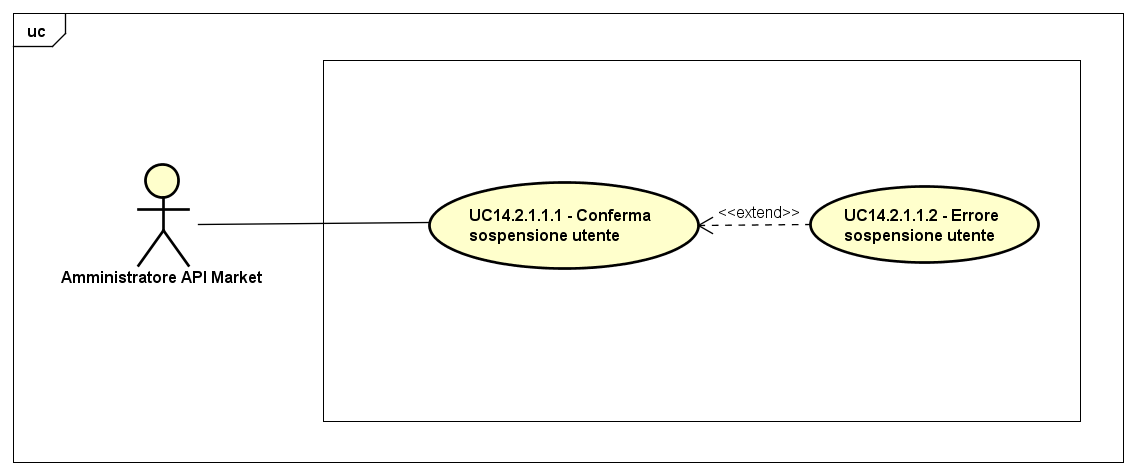
\includegraphics[scale=0.45]{UML/UC14_2_1_1.png}
	\caption{UC14.2.1.1: Sospensione utente}
\end{figure}

\begin{minipage}{\linewidth}
	\begin{tabular}{ l | p{11cm}}
		\hline
		\rowcolor{Gray}
		\multicolumn{2}{c}{UC14.2.1.1 - Sospensione utente} \\
		\hline
		\textbf{Attori} & Amministratore API Market \\
		\textbf{Descrizione} & L'attore sospende l'utente scelto (impedisce da parte sua l'uso delle API acquistate, e da parte degli altri utente l'uso delle API da lui registrate) \\
		\textbf{Pre-Condizioni} & L'attore si trova nella schermata relativa alla moderazione dell'utenza ed ha scelto un utente \\
		\textbf{Post-Condizioni} & L'attore ha sospeso l'utente scelto \\
		\textbf{Scenario Principale} & 
		\begin{enumerate*}[label=(\arabic*.),itemjoin={\newline}]
			\item L'attore può confermare la sospensione dell'utente scelto (UC14.2.1.1.1)
		\end{enumerate*}\\
		\textbf{Scenari Alternativi} & 
		\begin{enumerate*}[label=(\arabic*.),itemjoin={\newline}]
			\item L'attore, dopo aver confermato la sospensione dell'utente scelto, può visualizzare un messaggio di errore informativo e la sospensione non avviene (UC14.2.1.1.2)
		\end{enumerate*}\\
	\end{tabular}
\end{minipage}

\subparagraph{Caso d'uso UC14.2.1.1.1: Conferma sospensione utente}
\label{UC14_2_1_1_1}

\begin{minipage}{\linewidth}
	\begin{tabular}{ l | p{11cm}}
		\hline
		\rowcolor{Gray}
		\multicolumn{2}{c}{UC14.2.1.1.1 - Conferma sospensione utente} \\
		\hline
		\textbf{Attori} & Amministratore API Market \\
		\textbf{Descrizione} & L'attore conferma la sospensione dell'utente scelto e visualizza un messaggio di successo \\
		\textbf{Pre-Condizioni} & L'attore si trova nella schermata relativa alla moderazione dell'utenza ed ha scelto un utente \\
		\textbf{Post-Condizioni} & L'attore ha confermato la sospensione dell'utente scelto \\
		\textbf{Scenario Principale} & 
		\begin{enumerate*}[label=(\arabic*.),itemjoin={\newline}]
			\item L'attore conferma la sospensione dell'utente scelto e visualizza un messaggio di successo
		\end{enumerate*}\\
	\end{tabular}
\end{minipage}

\subparagraph{Caso d'uso UC14.2.1.1.2: Errore sospensione utente}
\label{UC14_2_1_1_2}

\begin{minipage}{\linewidth}
	\begin{tabular}{ l | p{11cm}}
		\hline
		\rowcolor{Gray}
		\multicolumn{2}{c}{UC14.2.1.1.2 - Errore sospensione utente} \\
		\hline
		\textbf{Attori} & Amministratore API Market \\
		\textbf{Descrizione} & L'attore visualizza un messaggio di errore informativo e la sospensione dell'utente scelto non avviene \\
		\textbf{Pre-Condizioni} & L'attore ha confermato la sospensione dell'utente scelto ma si è verificato un errore \\
		\textbf{Post-Condizioni} & L'attore ha visualizzato un messaggio di errore informativo \\
		\textbf{Scenario Principale} & 
		\begin{enumerate*}[label=(\arabic*.),itemjoin={\newline}]
			\item L'attore può visualizzare un messaggio di errore informativo e la sospensione dell'utente scelto non avviene
		\end{enumerate*}\\
	\end{tabular}
\end{minipage}

\newpage
\subparagraph{Caso d'uso UC14.2.1.2: Sospensione pagamenti verso utente}
\label{UC14_2_1_2}
\begin{figure}[ht]
	\centering
	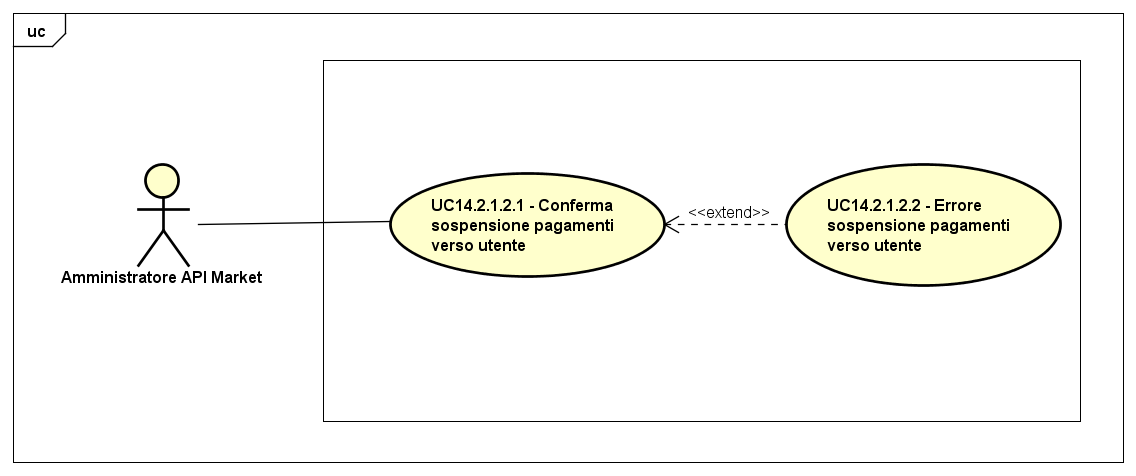
\includegraphics[scale=0.45]{UML/UC14_2_1_2.png}
	\caption{UC14.2.1.2: Sospensione pagamenti verso utente}
\end{figure}

\begin{minipage}{\linewidth}
	\begin{tabular}{ l | p{11cm}}
		\hline
		\rowcolor{Gray}
		\multicolumn{2}{c}{UC14.2.1.2 - Sospensione pagamenti verso utente} \\
		\hline
		\textbf{Attori} & Amministratore API Market \\
		\textbf{Descrizione} & L'attore sospende i pagamenti verso l'utente scelto \\
		\textbf{Pre-Condizioni} & L'attore si trova nella schermata relativa alla moderazione dell'utenza ed ha scelto un utente \\
		\textbf{Post-Condizioni} & L'attore ha sospeso i pagamenti verso l'utente scelto \\
		\textbf{Scenario Principale} & 
		\begin{enumerate*}[label=(\arabic*.),itemjoin={\newline}]
			\item L'attore può sospendere i pagamenti verso l'utente scelto (UC14.2.1.2.1)
		\end{enumerate*}\\
		\textbf{Scenari Alternativi} & 
		\begin{enumerate*}[label=(\arabic*.),itemjoin={\newline}]
			\item L'attore, dopo aver confermato la sospensione dei pagamenti verso l'utente scelto, può visualizzare un messaggio di errore informativo e la sospensione dei pagamenti non avviene (UC14.2.1.2.2)
		\end{enumerate*}\\
	\end{tabular}
\end{minipage}

\subparagraph{Caso d'uso UC14.2.1.2.1: Conferma sospensione pagamenti verso utente}
\label{UC14_2_1_2_1}

\begin{minipage}{\linewidth}
	\begin{tabular}{ l | p{11cm}}
		\hline
		\rowcolor{Gray}
		\multicolumn{2}{c}{UC14.2.1.2.1 - Conferma sospensione pagamenti verso utente} \\
		\hline
		\textbf{Attori} & Amministratore API Market \\
		\textbf{Descrizione} & L'attore conferma la sospensione dei pagamenti verso l'utente scelto e visualizza un messaggio di successo \\
		\textbf{Pre-Condizioni} & L'attore si trova nella schermata relativa alla moderazione dell'utenza ed ha scelto un utente \\
		\textbf{Post-Condizioni} & L'attore ha confermato la sospensione dei pagamenti verso l'utente scelto \\
		\textbf{Scenario Principale} & 
		\begin{enumerate*}[label=(\arabic*.),itemjoin={\newline}]
			\item L'attore conferma la sospensione dei pagamenti verso l'utente scelto e visualizza un messaggio di successo
		\end{enumerate*}\\
	\end{tabular}
\end{minipage}

\subparagraph{Caso d'uso UC14.2.1.2.2: Errore sospensione pagamenti verso utente}
\label{UC14_2_1_2_2}

\begin{minipage}{\linewidth}
	\begin{tabular}{ l | p{11cm}}
		\hline
		\rowcolor{Gray}
		\multicolumn{2}{c}{UC14.2.1.2.2 - Errore sospensione pagamenti verso utente} \\
		\hline
		\textbf{Attori} & Amministratore API Market \\
		\textbf{Descrizione} & L'attore visualizza un messaggio di errore informativo e la sospensione dei pagamenti verso l'utente scelto non avviene \\
		\textbf{Pre-Condizioni} & L'attore ha confermato la sospensione dei pagamenti verso l'utente scelto ma si è verificato un errore \\
		\textbf{Post-Condizioni} & L'attore ha visualizzato un messaggio di errore informativo \\
		\textbf{Scenario Principale} & 
		\begin{enumerate*}[label=(\arabic*.),itemjoin={\newline}]
			\item L'attore, può visualizzare un messaggio di errore informativo e la sospensione dei pagamenti verso l'utente scelto non avviene
		\end{enumerate*}\\
	\end{tabular}
\end{minipage}

\subparagraph{Caso d'uso UC14.2.1.3: Revoca sospensione utente}
\label{UC14_2_1_3}

\begin{minipage}{\linewidth}
	\begin{tabular}{ l | p{11cm}}
		\hline
		\rowcolor{Gray}
		\multicolumn{2}{c}{UC14.2.1.3 - Revoca sospensione utente} \\
		\hline
		\textbf{Attori} & Amministratore API Market \\
		\textbf{Descrizione} & L'attore revoca la sospensione dell'utente scelto, ricevendo un messaggio di successo \\
		\textbf{Pre-Condizioni} & L'attore si trova nella schermata relativa alla moderazione dell'utenza ed ha scelto un utente \\
		\textbf{Post-Condizioni} & L'attore ha revocato la sospensione dell'utente scelto, ricevendo un messaggio di successo \\
		\textbf{Scenario Principale} & 
		\begin{enumerate*}[label=(\arabic*.),itemjoin={\newline}]
			\item L'attore può revocare la sospensione dell'utente scelto, ricevendo un messaggio di successo
		\end{enumerate*}\\
	\end{tabular}
\end{minipage}

\subparagraph{Caso d'uso UC14.2.1.4: Revoca sospensione pagamenti verso utente}
\label{UC14_2_1_4}

\begin{minipage}{\linewidth}
	\begin{tabular}{ l | p{11cm}}
		\hline
		\rowcolor{Gray}
		\multicolumn{2}{c}{UC14.2.1.4 - Revoca sospensione pagamenti verso utente} \\
		\hline
		\textbf{Attori} & Amministratore API Market \\
		\textbf{Descrizione} & L'attore revoca la sospensione dei pagamenti verso l'utente scelto, ricevendo un messaggio di successo \\
		\textbf{Pre-Condizioni} & L'attore si trova nella schermata relativa alla moderazione dell'utenza ed ha scelto un utente \\
		\textbf{Post-Condizioni} & L'attore ha revocato la sospensione dei pagamenti verso l'utente scelto, ricevendo un messaggio di successo \\
		\textbf{Scenario Principale} & 
		\begin{enumerate*}[label=(\arabic*.),itemjoin={\newline}]
			\item L'attore può revocare la sospensione dei pagamenti verso l'utente scelto, ricevendo un messaggio di successo
		\end{enumerate*}\\
	\end{tabular}
\end{minipage}

\newpage
\subparagraph{Caso d'uso UC14.2.1.5: Cancellazione utente}
\label{UC14_2_1_5}
\begin{figure}[ht]
	\centering
	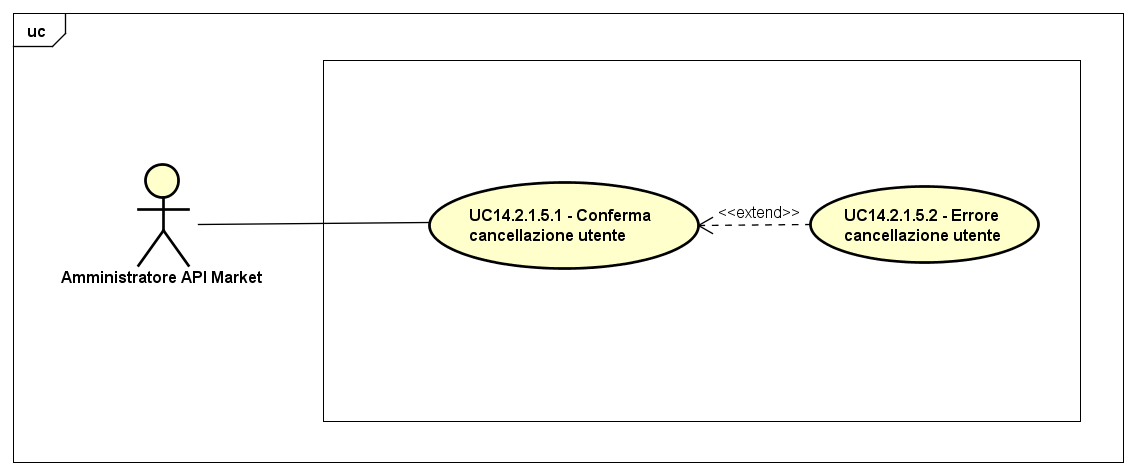
\includegraphics[scale=0.45]{UML/UC14_2_1_5.png}
	\caption{UC14.2.1.5: Cancellazione utente}
\end{figure}

\begin{minipage}{\linewidth}
	\begin{tabular}{ l | p{11cm}}
		\hline
		\rowcolor{Gray}
		\multicolumn{2}{c}{UC14.2.1.5 - Cancellazione utente} \\
		\hline
		\textbf{Attori} & Amministratore API Market \\
		\textbf{Descrizione} & L'attore imposta lo status dell'utente scelto come cancellato \\
		\textbf{Pre-Condizioni} & L'attore si trova nella schermata relativa alla moderazione dell'utenza ed ha scelto un utente \\
		\textbf{Post-Condizioni} & L'attore ha impostato lo status dell'utente scelto come cancellato \\
		\textbf{Scenario Principale} & 
		\begin{enumerate*}[label=(\arabic*.),itemjoin={\newline}]
			\item L'attore può confermare la cancellazione dell'utente scelto (UC14.2.1.5.1)
		\end{enumerate*}\\
		\textbf{Scenari Alternativi} & 
		\begin{enumerate*}[label=(\arabic*.),itemjoin={\newline}]
			\item L'attore, dopo aver confermato la cancellazione dell'utente scelto, può visualizzare un messaggio di errore informativo e la cancellazione non avviene (UC14.2.1.5.2)
		\end{enumerate*}\\
	\end{tabular}
\end{minipage}

\subparagraph{Caso d'uso UC14.2.1.5.1: Conferma cancellazione utente}
\label{UC14_2_1_5_1}

\begin{minipage}{\linewidth}
	\begin{tabular}{ l | p{11cm}}
		\hline
		\rowcolor{Gray}
		\multicolumn{2}{c}{UC14.2.1.5.1 - Conferma cancellazione utente} \\
		\hline
		\textbf{Attori} & Amministratore API Market \\
		\textbf{Descrizione} & L'attore conferma la cancellazione dell'utente scelto e visualizza un messaggio di successo \\
		\textbf{Pre-Condizioni} & L'attore si trova nella schermata relativa alla moderazione dell'utenza ed ha scelto un utente \\
		\textbf{Post-Condizioni} & L'attore ha confermato la cancellazione dell'utente scelto \\
		\textbf{Scenario Principale} & 
		\begin{enumerate*}[label=(\arabic*.),itemjoin={\newline}]
			\item L'attore conferma la cancellazione dell'utente scelto e visualizza un messaggio di successo
		\end{enumerate*}\\
	\end{tabular}
\end{minipage}

\subparagraph{Caso d'uso UC14.2.1.5.2: Errore cancellazione utente}
\label{UC14_2_1_5_2}

\begin{minipage}{\linewidth}
	\begin{tabular}{ l | p{11cm}}
		\hline
		\rowcolor{Gray}
		\multicolumn{2}{c}{UC14.2.1.5.2 - Errore cancellazione utente} \\
		\hline
		\textbf{Attori} & Amministratore API Market \\
		\textbf{Descrizione} & L'attore visualizza un messaggio di errore informativo e la cancellazione dell'utente scelto non avviene \\
		\textbf{Pre-Condizioni} & L'attore ha confermato la cancellazione dell'utente scelto ma si è verificato un errore \\
		\textbf{Post-Condizioni} & L'attore ha visualizzato un messaggio di errore informativo \\
		\textbf{Scenario Principale} & 
		\begin{enumerate*}[label=(\arabic*.),itemjoin={\newline}]
			\item L'attore può visualizzare un messaggio di errore informativo e la cancellazione dell'utente scelto non avviene
		\end{enumerate*}\\
	\end{tabular}
\end{minipage}

